\documentclass[conference,a4paper,twoside]{IEEEtran}
\usepackage[utf8]{inputenc}
\usepackage{amsmath}
\usepackage{amsfonts}
\usepackage{amssymb}
\usepackage{graphicx}
\usepackage[space]{grffile}
\graphicspath{figures/}
\usepackage{import}
\usepackage{url}
\usepackage{hyperref}
\usepackage{subcaption}
\usepackage{tikz}
\usepackage{siunitx}
\usepackage[disable]{todonotes}
\let\OldTodo\todo
\renewcommand{\todo}{\OldTodo[inline]}
\newcommand{\todolater}[1]{}%\todo
\RequirePackage[date=terse, isbn=true, doi=true, url=false, urldate=iso8601, maxbibnames=9, backref=false, backend=bibtex, style=ieee]{biblatex}
\addbibresource{securityupdates.bib}
\renewcommand{\bibfont}{\small}

\AtEveryBibitem{% Clean up the bibtex rather than editing it
 \clearname{editor} % remove editors
}

\author{Daniel R.\ Thomas, Alastair R.\ Beresford, Daniel T.\ Wagner and Andrew Rice}

\newcommand{\daNumDataPoints}{153 Billion}
\newcommand{\daNumStartedApps}{122\,000}
\newcommand{\daNumInstalledApps}{175\,000}
\newcommand{\daNumVulnsUsed}{11}
\newcommand{\daSigNumDevices}{100}
\newcommand{\daSigNumDays}{100}
\newcommand{\daNumManufacturers}{261}
\newcommand{\daNumSigManufacturers}{9}
\newcommand{\daNumModels}{2\,380}
\newcommand{\daNumSigModels}{15}
\newcommand{\daOSVersionPercValidLines}{99.5\%}
\newcommand{\daOSTotalDaysData}{1\,140\,000}
\newcommand{\daMeanInsecurityPerc}{$87.3 \pm 0.0\%$}
\newcommand{\daMeanOutstandingVulnerabilities}{0.637}
\newcommand{\daUpdatedness}{$0.0558 \pm 0.0002$}
\newcommand{\daSecurityScore}{$2.75 \pm 0.00$}
\newcommand{\daNumFullVersions}{1\,140}
\newcommand{\daNumOSVersions}{45}
\newcommand{\daNumSigOSVersions}{23}
\newcommand{\daNumAPIVersions}{15}
\newcommand{\daNumFullVersionUpdates}{4\,220}
\newcommand{\daNumOSVersionUpdates}{3\,560}
\newcommand{\daNumFullOnlyVersionUpdates}{640}
\newcommand{\daNumSecurityUpdates}{1\,110}
\newcommand{\daNumPossibleSecurityUpdates}{2\,140}
\newcommand{\daTabSecScoresmanufacturer}{\begin{table} \centering \begin{tabular}{l|c|c|c|c} Name & $f$ & $u$ & $m$ & \textbf{Security score} \\ &&&& (out of 10) \\ \hline LG & $0.12 \pm 0.00$ & $0.32 \pm 0.00$ & 0.74 & $3.38 \pm 0.01$ \\  Motorola & $0.16 \pm 0.00$ & $0.13 \pm 0.00$ & 0.77 & $2.93 \pm 0.01$ \\  other & $0.13 \pm 0.00$ & $0.06 \pm 0.00$ & 0.64 & $2.75 \pm 0.00$ \\  Samsung & $0.14 \pm 0.00$ & $0.05 \pm 0.00$ & 0.71 & $2.67 \pm 0.00$ \\  Sony & $0.13 \pm 0.00$ & $0.18 \pm 0.00$ & 1.02 & $2.64 \pm 0.01$ \\  HTC & $0.14 \pm 0.00$ & $0.09 \pm 0.00$ & 0.89 & $2.55 \pm 0.00$ \\  asus & $0.15 \pm 0.00$ & $0.56 \pm 0.01$ & 6.06 & $2.30 \pm 0.02$ \\  Symphony & $0.00 \pm 0.00$ & $0.04 \pm 0.00$ & 4.79 & $0.19 \pm 0.00$ \\  walton & $0.00 \pm 0.00$ & $0.04 \pm 0.00$ & 5.79 & $0.14 \pm 0.01$ \\ \end{tabular} \caption{Security scores for manufacturers} \label{tab:sec_manufacturer} \end{table}}
\newcommand{\daTabSecScoresmodel}{\begin{table} \centering \begin{tabular}{l|c|c|c|c} Name & $f$ & $u$ & $m$ & \textbf{Security score} \\ &&&& (out of 10) \\ \hline Galaxy Nexus & $0.53 \pm 0.00$ & $0.53 \pm 0.01$ & 1.53 & $4.80 \pm 0.03$ \\  Nexus 4 & $0.23 \pm 0.00$ & $0.82 \pm 0.01$ & 6.06 & $3.39 \pm 0.04$ \\  Nexus 7 & $0.19 \pm 0.00$ & $0.74 \pm 0.01$ & 5.92 & $3.02 \pm 0.04$ \\  other & $0.13 \pm 0.00$ & $0.12 \pm 0.00$ & 0.64 & $2.94 \pm 0.00$ \\  Desire HD & $0.08 \pm 0.00$ & $0.05 \pm 0.00$ & 0.39 & $2.91 \pm 0.02$ \\  HTC Sensation & $0.36 \pm 0.00$ & $0.01 \pm 0.01$ & 1.59 & $2.47 \pm 0.02$ \\  GT-I9100 & $0.22 \pm 0.00$ & $0.02 \pm 0.00$ & 1.20 & $2.33 \pm 0.01$ \\  HTC Desire S & $0.02 \pm 0.00$ & $0.02 \pm 0.00$ & 1.00 & $1.75 \pm 0.01$ \\  GT-N7000 & $0.25 \pm 0.00$ & $0.00 \pm 0.00$ & 2.52 & $1.43 \pm 0.02$ \\  GT-P1000 & $0.01 \pm 0.00$ & $0.00 \pm 0.01$ & 1.73 & $0.94 \pm 0.02$ \\  GT-I9300 & $0.15 \pm 0.00$ & $0.01 \pm 0.00$ & 6.15 & $0.64 \pm 0.01$ \\  GT-I9505 & $0.00 \pm 0.00$ & $0.18 \pm 0.00$ & 6.77 & $0.55 \pm 0.01$ \\  GT-N7100 & $0.07 \pm 0.00$ & $0.00 \pm 0.01$ & 6.91 & $0.28 \pm 0.02$ \\  HTC Desire HD & $0.00 \pm 0.00$ & $0.00 \pm 0.01$ & 3.05 & $0.27 \pm 0.02$ \\ \end{tabular} \caption{Security scores for models} \label{tab:sec_model} \end{table}}
\newcommand{\daTabSecScoressummary}{\begin{table} \centering \begin{tabular}{l|c|c|c|c} Name & $f$ & $u$ & $m$ & \textbf{Security score} \\ &&&& (out of 10) \\ \hline nexus & $0.36 \pm 0.00$ & $0.51 \pm 0.00$ & 0.68 & $5.01 \pm 0.01$ \\  notnexus & $0.12 \pm 0.00$ & $0.04 \pm 0.00$ & 0.64 & $2.67 \pm 0.00$ \\ \end{tabular} \caption{Security scores for nexus} \label{tab:sec_summary} \end{table}}
\newcommand{\daUpdatednessPerc}{$5.58 \pm 0.02\%$}
\newcommand{\daNumOSDevices}{19\,000}
\newcommand{\daSigNumDevicesDay}{20}
\newcommand{\daSigNumDeviceDays}{10\,000}
\newcommand{\daTabAndVulns}{\begin{table} \centering \begin{tabular}{l|c|l} Vulnerability & Date known & How known \\ \hline KillingInTheNameOf psneuter ashmem & 2010-07-13 & Fixed on \\ exploid udev & 2010-07-15 & Discovered on \\ RageAgainstTheCage adb & 2010-08-21 & Discovered on \\ levitator & 2011-03-10 & Discovered on \\ Gingerbreak & 2011-04-18 & Fixed on \\ zergRush & 2011-10-06 & Discovered on \\ APK duplicate file & 2013-02-18 & Discovered on \\ APK unchecked name & 2013-06-30 & Discovered on \\ APK unsigned shorts & 2013-07-03 & Fixed on \\ keystore buffer & 2013-09-09 & Discovered on \\ TwerkMyMoto & 2013-11-24 & Discovered on \\ vold asec & 2014-01-27 & Fixed on \\\end{tabular} \caption{Root equivalent vulnerabilities in Android} \label{tab:andvulns} \end{table}}
\newcommand{\daOSYearsOfData}{3}
\newcommand{\daSecScoreBestmanufacturer}{LG}
\newcommand{\daSecScoreWorstmanufacturer}{walton}
\newcommand{\daSecScoreBestmodel}{Galaxy Nexus}
\newcommand{\daSecScoreWorstmodel}{HTC Desire HD A9191}
\newcommand{\daSecScoreBestsummary}{nexus}
\newcommand{\daSecScoreWorstsummary}{notnexus}
\newcommand{\daSecScoreBestmanufacturerScore}{$3.38 \pm 0.01$}
\newcommand{\daSecScoreWorstmanufacturerScore}{$0.139 \pm 0.006$}
\newcommand{\daSecScoreBestmodelScore}{$4.8 \pm 0.0$}
\newcommand{\daSecScoreWorstmodelScore}{$0.274 \pm 0.020$}
\newcommand{\daSecScoreBestsummaryScore}{$4.1 \pm 0.0$}
\newcommand{\daSecScoreWorstsummaryScore}{$2.9 \pm 0.0$}
\newcommand{\daVulnFree}{$0.127 \pm 0.000$}
\newcommand{\daAdbEnabledPerc}{$19.5 \pm 0.0\%$}
\newcommand{\daNumUpdatesUpgrades}{3\,330}
\newcommand{\daNumUpdatesDowngrades}{147}
\newcommand{\daPercUpdatesDowngrades}{$3.58 \pm 0.3\%$}
\newcommand{\daStartDate}{2011-07-01}
\newcommand{\daEndDate}{2014-11-07}
\newcommand{\daNumOperators}{1\,390}
\newcommand{\daTabSecScoresoperator}{\begin{table} \centering \begin{tabular}{l|c|c|c|c} Name & $f$ & $u$ & $m$ & \textbf{Security score} \\ &&&& (out of 10) \\ \hline O2 uk & $0.25 \pm 0.00$ & $0.12 \pm 0.00$ & 0.37 & $3.79 \pm 0.01$ \\  T-Mobile & $0.19 \pm 0.00$ & $0.18 \pm 0.00$ & 0.48 & $3.57 \pm 0.01$ \\  Orange & $0.21 \pm 0.00$ & $0.09 \pm 0.00$ & 0.39 & $3.52 \pm 0.02$ \\  Sprint & $0.18 \pm 0.00$ & $0.11 \pm 0.00$ & 0.44 & $3.41 \pm 0.01$ \\  3 & $0.15 \pm 0.00$ & $0.09 \pm 0.00$ & 0.49 & $3.15 \pm 0.01$ \\  AT\&T & $0.12 \pm 0.00$ & $0.08 \pm 0.00$ & 0.43 & $3.08 \pm 0.01$ \\  Vodafone uk & $0.13 \pm 0.00$ & $0.10 \pm 0.00$ & 0.52 & $3.07 \pm 0.01$ \\  Verizon & $0.18 \pm 0.00$ & $0.09 \pm 0.00$ & 0.81 & $2.82 \pm 0.01$ \\  unknown & $0.10 \pm 0.00$ & $0.22 \pm 0.00$ & 1.08 & $2.57 \pm 0.01$ \\  n Telenor & $0.03 \pm 0.00$ & $0.10 \pm 0.00$ & 1.42 & $1.59 \pm 0.01$ \\  Airtel & $0.06 \pm 0.00$ & $0.03 \pm 0.00$ & 1.93 & $1.10 \pm 0.01$ \\  Grameenphone & $0.01 \pm 0.00$ & $0.02 \pm 0.00$ & 1.99 & $0.80 \pm 0.00$ \\  Robi & $0.00 \pm 0.00$ & $0.04 \pm 0.00$ & 2.19 & $0.73 \pm 0.01$ \\  banglalink & $0.00 \pm 0.00$ & $0.03 \pm 0.00$ & 2.90 & $0.40 \pm 0.00$ \\ \end{tabular} \caption{Security scores for operators} \label{tab:sec_operator} \end{table}}
\newcommand{\daSecScoreBestoperator}{O2 uk}
\newcommand{\daSecScoreBestoperatorScore}{$3.79 \pm 0.01$}
\newcommand{\daSecScoreWorstoperator}{banglalink}
\newcommand{\daSecScoreWorstoperatorScore}{$0.4 \pm 0.0$}
\newcommand{\daNumSigOperators}{14}
\newcommand{\daMonthsDevices}{1\,600}
\newcommand{\daMonths}{6}
\newcommand{\daSigVersionPerc}{1\%}
\newcommand{\daSigVersionDays}{10}
\newcommand{\daNumDeviceDataDevices}{50}
\newcommand{\daNumSigFullVersions}{83}
\newcommand{\daSecScoreBestmanufacturerNumFullVersions}{104}
\newcommand{\daSecScoreworstmanufacturerNumFullVersions}{239}
\newcommand{\daSecScoreBestmodelNumFullVersions}{49}
\newcommand{\daSecScoreworstmodelNumFullVersions}{2}
\newcommand{\daSecScoreBestsummaryNumFullVersions}{73}
\newcommand{\daSecScoreworstsummaryNumFullVersions}{1057}
\newcommand{\daSecScoreBestoperatorNumFullVersions}{88}
\newcommand{\daSecScoreworstoperatorNumFullVersions}{89}
\newcommand{\daSecScoreWorstmanufacturerNumFullVersions}{20}
\newcommand{\daSecScoreWorstmodelNumFullVersions}{2}
\newcommand{\daSecScoreWorstsummaryNumFullVersions}{1103}
\newcommand{\daSecScoreWorstoperatorNumFullVersions}{59}
\newcommand{\daFullDeployedAt}{95\%}
\newcommand{\daOSCurveFitParamFirst}{87.5}
\newcommand{\daOSCurveFitParamSecond}{\num{0.00315}}
\newcommand{\daOSCurveFitRMSE}{0.114}
\newcommand{\daAPICurveFitParamFirst}{110}
\newcommand{\daAPICurveFitParamSecond}{\num{0.00315}}
\newcommand{\daAPICurveFitRMSE}{0.116}
\newcommand{\daOSCurvePolyRMSE}{0.115}
\newcommand{\daOSCurveSplineRMSE}{0.115}
\newcommand{\daOSCurveHalfDeployed}{$308 \pm 81$}
\newcommand{\daOSCurveFullDeployed}{$1\,040 \pm 236\,000$}
\newcommand{\daAPICurvePolyRMSE}{0.117}
\newcommand{\daAPICurveSplineRMSE}{0.117}
\newcommand{\daAPICurveHalfDeployed}{$330 \pm 84$}
\newcommand{\daAPICurveFullDeployed}{$1\,060 \pm 236\,000$}
\newcommand{\daVulnAPKDuplicateFileOctoberPerc}{91.5\%}
\newcommand{\daNumUpdatesBigUpgrades}{778}
\newcommand{\daNumUpdatesSkippedBig}{3}
\newcommand{\daPercBigUpgrades}{$18.9 \pm 0.7\%$}
\newcommand{\daUpdatesPerYear}{$1.35 \pm 0.02$}
\newcommand{\daOSMonthsOfData}{40}
\newcommand{\daMeanInsecurityPercNominal}{87.3\%}
\newcommand{\daVulnFreeNominal}{0.127}
\newcommand{\daUpdatednessNominal}{0.0558}
\newcommand{\daUpdatednessPercNominal}{5.58\%}
\newcommand{\daSecurityScoreNominal}{2.75}
\newcommand{\daUpdatesPerYearNominal}{1.35}
\newcommand{\daOSCurveHalfDeployedNominal}{308}
\newcommand{\daOSCurveFullDeployedNominal}{1\,040}
\newcommand{\daAPICurveHalfDeployedNominal}{330}
\newcommand{\daAPICurveFullDeployedNominal}{1\,060}
\newcommand{\daSecScoreBestoperatorScoreNominal}{3.79}
\newcommand{\daSecScoreWorstoperatorScoreNominal}{0.4}
\newcommand{\daSecScoreBestmodelScoreNominal}{4.8}
\newcommand{\daSecScoreWorstmodelScoreNominal}{0.274}
\newcommand{\daAdbEnabledPercNominal}{19.5\%}
\newcommand{\daSecScoreBestmanufacturerScoreNominal}{3.38}
\newcommand{\daSecScoreWorstmanufacturerScoreNominal}{0.139}
\newcommand{\daUpdatesPerMonthPerVersion}{$3.62 \pm 0.06$}
\newcommand{\daNumUpdateFullOnly}{637}
\newcommand{\daVulnZergRushMonthsDefFixDeployed}{27.3}
\newcommand{\daUpdatesPerMonthPerVersionNominal}{3.62}
\newcommand{\daPercBigUpgradesNominal}{18.9\%}
\newcommand{\daPercUpdatesDowngradesNominal}{3.58\%}

\newcommand{\da}{Device Analyzer}
\newcommand{\dafoot}{\textsuperscript{\ref{foot:dadata}}}
\newcommand{\avoNumSubmitters}{7}
\newcommand{\avoTotalExternalLines}{25 Million}
\newcommand{\avoNumExternalProjects}{176}
\newcommand{\avoNumBigExternalLinesOfCode}{25 Million}
\newcommand{\avoBigExternalLinesOfCodePerc}{99.7\%}
\newcommand{\avoNumVulnerabilities}{32}
\newcommand{\avoNumVulnAllAndroid}{15}
\newcommand{\avoNumVulnSpecific}{17}
\newcommand{\avoStartDate}{2013-08-28}
\newcommand{\avoEndDate}{2015-03-24}
\newcommand{\avoFirstDataDateMonth}{July 2010}
\newcommand{\avoFirstDataDate}{2010-07-13}
\newcommand{\avoLastDataDateMonth}{March 2015}
\newcommand{\avoLastDataDate}{2015-03-12}
\newcommand{\avoVulnsPerYearNominal}{6.86}
\newcommand{\avoVulnsPerYear}{$6.86 \pm 1.21$}
\newcommand{\avoVulnsPerYearAllAndroidNominal}{3.21}
\newcommand{\avoVulnsPerYearAllAndroid}{$3.21 \pm 0.83$}
\newcommand{\avoVulnsPerYearTwosfNominal}{6.9}
\newcommand{\avoVulnsPerYearTwosf}{$6.9 \pm 1.2$}
\newcommand{\avoVulnsPerYearAllAndroidTwosfNominal}{3.2}
\newcommand{\avoVulnsPerYearAllAndroidTwosf}{$3.2 \pm 0.0$}
\newcommand{\avoTabAndVulns}{\begin{table} \centering \small \begin{tabular}{l|l|c|c} Vulnerability & How known & Date & Categories\\ \hline KillingInTheNameOf & Fixed on & 2010-07-13 & system, kernel\\ exploid udev & Discovered on & 2010-07-15 & kernel\\ levitator & Discovered on & 2011-03-10 & kernel\\ Gingerbreak & Fixed on & 2011-04-18 & system\\ zergRush & Discovered on & 2011-10-06 & system\\ APK duplicate file & Discovered on & 2013-02-18 & signature\\ APK unchecked name & Discovered on & 2013-06-30 & signature\\ APK unsigned shorts & Fixed on & 2013-07-03 & signature\\ vold asec & Fixed on & 2014-01-27 & system\\ Fake ID & Fixed on & 2014-04-17 & signature\\ TowelRoot & Discovered on & 2014-05-03 & kernel\\\end{tabular} \caption{Critical vulnerabilities in Android} \label{tab:andvulns} \end{table}}
\newcommand{\avoNumBigExternalProjects}{40}
\newcommand{\avoNumAnalysedExternalProjects}{28}
\newcommand{\avoNumAnalysedExternalLinesOfCode}{6 Million}
\newcommand{\avoAnalysedExternalLinesOfCodePerc}{24.9\%}
\newcommand{\avoBigExternalMedianVersions}{2.0}
\newcommand{\avoBigExternalMeanVersionsNominal}{2.57}
\newcommand{\avoBigExternalMeanVersions}{$2.57 \pm 1.84$}
\newcommand{\avoBigExternalTotalVersions}{72}

\newcommand{\avo}{AVO}
\newcommand{\percMarketShare}{83.6\%~\footnote{\url{http://www.theinquirer.net/inquirer/news/2379036/android-hits-836-percent-marketshare-while-ios-windows-and-blackberry-slide}}}
\newcommand{\daNumDevices}{\daNumOSDevices}
\newcommand{\daDeviceDays}{\daOSTotalDaysData}
% Num versions since \daStartDate
\newcommand{\opensslNumVersions}{59}
\newcommand{\linuxNumVersions}{618}
\newcommand{\linuxMeanUpdateLatency}{$137 \pm 48$}
\newcommand{\opensslMeanUpdateLatency}{$120 \pm 55$}
\newcommand{\bouncycastleNumVersions}{6}
\newcommand{\bouncycastleMeanUpdateLatency}{$239 \pm 78$}
\newcommand{\linuxMeanUpdateLatencyNominal}{137}
\newcommand{\opensslMeanUpdateLatencyNominal}{120}
\newcommand{\bouncycastleMeanUpdateLatencyNominal}{239}

\newcommand{\otherProjNum}{\avoNumExternalProjects}%TODO check we are doing the right calculation here and not overcounting

% Blinding function
\newcommand{\identifying}[1]{}%{#1}%
\newcommand{\blindauthors}[1]{Paper \#59}%{#1}%

\begin{document}
\title{Timeliness of security updates for Android}


% author names and affiliations
% use a multiple column layout for up to three different
% affiliations
\author{
\blindauthors{
\IEEEauthorblockN{Daniel R. Thomas,
Daniel T. Wagner,
Alastair R. Beresford,
Andrew Rice}
\IEEEauthorblockA{
Computer Laboratory\\
University of Cambridge\\
Cambridge, United Kingdom\\
Firstname.Lastname@cl.cam.ac.uk
}
}
}

% Terminology

% Android, Unix, adb
% update, release, patch: what do we actually mean and what relevance does that have to security?
% Device manufacturers
% Network operators
% Device model TODO check
% Device handset TODO check


\maketitle

% Hypothesis
% Attempts at fine grained restrictions on running arbitrary code are hampered by updates for security vulnerabilities not reaching users in a timely fashion.

\begin{abstract}
Modern smartphone operating systems protect users from malicious applications by providing a protected execution environment or sandbox.
This approach relies on the absence of active exploits which allow apps to break out of the sandbox.
Many such exploits have been found, and therefore the security of a smartphone operating system relies on the prompt delivery of security updates.
In this paper we tease apart the Android software ecosystem and quantify the extent to which the security sandbox provided by Android protects devices from malicious apps.
We analysed \da\ data from over \daOSYearsOfData\ years and \daNumOSDevices\ devices and found that on average \daMeanInsecurityPercNominal\ of devices were exposed to known root privilege vulnerabilities and only \daUpdatednessPercNominal\ of devices run the most recent version of Android.
We find there is significant variability in the timely delivery of security updates across different device manufacturers and mobile network operators, and we define a security metric to rank the performance of device manufacturers and network operators in our data set.
\end{abstract}

\section{Introduction}
%Android is the most popular smartphone operating system today with \percMarketShare\ marketshare.

Support for third-party apps is a key feature of modern smartphone operating systems.
Such apps are written by many developers from a wide range of backgrounds, which means neither operating system vendors nor users can fully trust app developers.
Therefore, in order to secure personal data and prevent theft, such as the sending of premium-rate text messages, operating system vendors provide a protected execution environment, or \emph{sandbox}, for apps.

In this paper we quantify the extent to which the app sandbox provided by Android protects devices from malicious apps attempting to gain control over the entire handset.
%We have analysed Android because it is the most popular smartphone operating system by market share (~\percMarketShare) and 
Previous research has shown that in 2012, between 36.7\%~\cite{Zhou2012b} and 40\%~\cite{Zhou2012a} of malware for Android contained exploits designed to enable a malicious app to break the sandbox.
What is not known however is the proportion of Android devices which are vulnerable to these exploits over time.
To the best of our knowledge, this is the first paper to provide detailed numbers.

Not all malicious apps need to break the sandbox in order to misbehave.
Indeed, the above figures suggest the majority of malicious apps do not attempt to do so.
We focus on the issue of apps breaking out of the sandbox because malware which is able to take full control of a handset can do significantly more harm and is much harder to remove.
Ordinary malware can be uninstalled by the user, or remotely by Google through the Play Store, and returns the device to a secure state. 
Removing an app which has used an exploit to take control of the handset is unlikely to return the device to secure state.
We describe our threat model and three attack vectors in detail in \S\ref{sec:threatmodel}.

The development of Android is distributed among many parties and the security of Android relies on many open source projects, include the Linux kernel, OpenSSL and BouncyCastle as well as Google who build the core platform. 
In addition, device manufacturers (we know of \daNumManufacturers\footnote{\label{foot:dadata}We computed this from the \da~\cite{Wagner2013} data, see \S\ref{sec:android_update_process}.}) and network operators (\daNumOperators\dafoot) may make further modifications before devices are shipped to customers. 
Understanding this ecosystem is important as device manufacturers have introduced additional vulnerabilities in the past~\cite{Grace2012}. 
We present a better understanding of both the ecosystem of Android development and associated vulnerabilities more fully in \S\ref{sec:android_ecosystem}.
 
\begin{figure}[h]
\centering
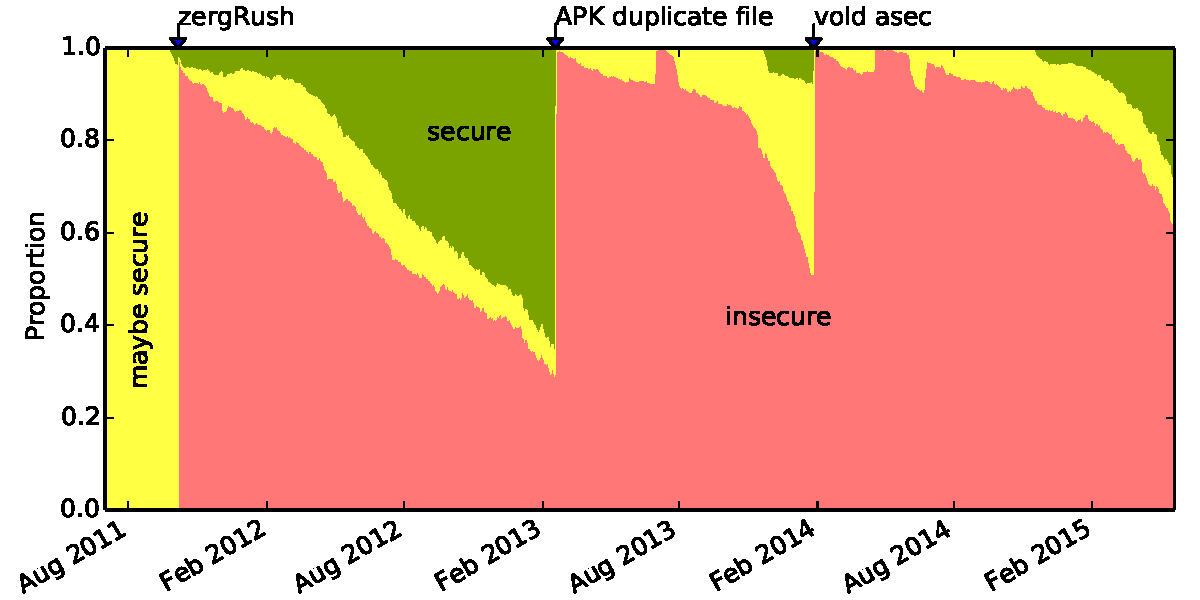
\includegraphics[width=\columnwidth]{figures/proportioninsecure}
\caption{Proportion of devices running insecure, maybe insecure and secure versions of Android against time.
The red vertical lines are caused by vulnerabilities being discovered with those which have the biggest impact annotated.
This graph is explained further in \S\ref{sec:exp:versionsecurity}.
}
\label{fig:proportioninsecure}
\end{figure}

In order to determine whether an individual smartphone is vulnerable to a particular exploit, we need to combine vulnerability data with the operating system version string and build number from the handset. 
For this we use handset data gathered from \daNumOSDevices\ devices in the \da~\cite{Wagner2013} project.
This analysis allows us to plot the proportion of Android devices in the \da\ data which were running versions of Android known to have vulnerabilities at the time and is shown in Figure~\ref{fig:proportioninsecure}.
The figure shows the proportion of devices split into three categories:
(1)~\emph{secure} because they are running a version of Android with no known vulnerabilities; 
(2)~\emph{insecure} because the device was running an insecure version of Android with a build released before the vulnerability was fixed or discovered; and 
(3)~\emph{maybe insecure} because the device is running a version of Android known to be insecure but has received an update which might contain a backported fix as we did not observe that build number until after the vulnerability was known.
Further analysis into the propagation of updates in Android is presented in \S\ref{sec:exp:android_ecosystem}.

It is clear from Figure~\ref{fig:proportioninsecure} that Android devices are often exposed to known security vulnerabilities.
One solution is regulation, and indeed there is ongoing legal action to force network operators to ship updates for security vulnerabilities~\cite{Soghoian2013}.\todolater{Check on the status of this legal action}
Many smartphones are sold on 12--24 month contracts, and yet our data shows many devices do not receive many security updates, with an overall average of \daUpdatesPerYearNominal\ per year. 
In contrast, Windows XP could be purchased for a one-off payment in October 2001 and received security updates until April 2014.

An alternative to regulation is access to publicly available data. 
Comparative data would provide an incentive to both device manufacturers and network operators to provide updates.
Currently corporate and public sector buyers are encouraged to purchase secure devices, but we have found little concrete guidance on the specific makes and models providing the best security. 
For example, CESG, which advises the UK government on how to secure its computer systems, recommends picking Android device models from device manufactures which are good at shipping security updates promptly~\cite{CESG2013} but it does not state which device manufacturers these are.
To address this, we developed a scoring system and provide numbers on the historic performance of device models in the \da\ project in~\S\ref{sec:security_scoring}.

In summary, the contributions of this paper are:
\begin{itemize}
 \item We characterise the Android update ecosystem, showing how updates flow between entities, and quantify vulnerabilities by determining what proportion of devices they affected and how that changes over time.
 \item We created an open database to collate quantitative information on vulnerabilities which affect Android, and investigate their time-lines.
 \item We measure the security of Android according to three metrics and compare different device manufacturers and device models to allow device purchasers to differentiate between them based on security.
\end{itemize}

\section{Threat model}
\label{sec:threatmodel}

In this paper we measure whether an attacker can take control of a handset by breaking out of the app sandbox on Android using a known vulnerability.
We consider three attack vectors.
The first attack vector is through the installation of a malicious app on the device.
Android devices support the installation of apps through a number of app marketplaces, email attachments, URLs and via the Android Debug Bridge (ADB).
By default, many Android devices with Google Play installed will prevent the installation of apps from other sources.

Controlling potential sources of app installation is a good security feature because app marketplaces provide additional protection to prevent the listing of malicious apps.
For example, the Google Play marketplace uses Bouncer to automatically analyse apps as well as removing any apps which are reported as malicious.
Nevertheless, Google Play is not immune: 0.02\% of apps are malicious~\cite{Zhou2012a}.
Alternative markets are also popular, particularly in countries such as China where the Google Play is not available. 
Previous work has shown that on alternative markets between 0.20\% and 0.47\% of apps are malicious~\cite{Zhou2012a}.

The second attack vector is to persuade an existing app to download and execute code at runtime.
The most direct method available to an attacker is to upload to a marketplace a seemingly innocent app which contains support for dynamic code loading from a remote server under control of the attacker.
Neither static nor dynamic analysis of this app by the marketplace will uncover any malicious code, since it does exist in the app binary.
Instead the attacker can chose to send a malicious payload directly to the app for execution at a later point in time. Note that dynamic code loading is not actually needed for this to work---it just makes the task easier---since previous work has shown that even on a platform such as iOS, which does not permit dynamic code loading, a ROP-based attack is relatively easy if the attacker creates an app with carefully crafted flaws~\cite{}.

Support for dynamic code loading on Android also supports the third attack vector in which the attacker injects malicious code directly into existing apps already installed on the handset. 
For example, the addJavascriptInterface vulnerability (CVE-2012-6636) allows Javascript running in an Android WebView to execute arbitrary code in the same process address space as the vulnerable app.
This attack works when: (1) the WebView has the Javascript-to-Java bridge enabled; and (2) the attacker is able to inject a malicious Javascript payload into the network traffic between the phone and the web server. 
Many apps are vulnerable to this type of attack because ad network libraries typically embed adverts into apps by displaying HTML and Javascript inside a WebView with the Javascript-to-Java bridge enabled. 
The fix for the addJavascriptInterface vulnerability breaks backwards compatibility, and therefore apps are only immune to this attack if their target API level is greater than 16 and they are running on an Android device with an OS version of 4.2 or greater.
Later analysis in Figure~\ref{fig:da_api} in this paper shows that 40\% of handsets connecting to the Google Play store are currently vulnerable to this attack.

\section{Data sources}
\label{sec:background}

We require two sources of data for this study: (1) information on the distribution of installed versions of Android over time across the Android ecosystem and (2) information on the critical vulnerabilities found to affect specific versions of Android.
These two datasets can then be combined to determine the proportion of handsets at risk of attack from specific vulnerabilities for particular periods of time.

\subsection{Versions of Android running on devices}

In our analysis we use historical data collected by the \da\ project~\cite{Wagner2013}.
Device Analyzer collects data from study participants who install the project Android app from the Google Play store.
Most study participants allow researchers around the world to access a subset of their device data, including the data presented in this paper.

The \da\ app collects a range of metadata from Android devices.\footnote{\url{https://deviceanalyzer.cl.cam.ac.uk/collected.html}}
For this paper, we extracted the build string and API version from the device log each day.
The API version is a positive integer which increases when new features are added to the API.
Consequently security (bug) fixes do not result in a change in the API version.
The build string is a user-readable version string.
Fortunately most (\daOSVersionPercValidLines) entries in the data have a build string of the form `x.y.z opaque\_marker' and so it is possible to extract the Android version number `x.y.z'.
On a large proportion of devices `opaque\_marker' is a well defined build number\footnote{\url{https://source.android.com/source/build-numbers.html}} however different device manufacturers use different schema.

The \da\ project has collected data from \daNumDevices\ devices with a total of \daDeviceDays\footnote{Here we are only counting devices and days for which we have valid OS version data.} device days. The majority of devices only contribute data for a short period of time, however \daMonthsDevices\ devices have contributed data for more than \daMonths~months.

Where possible we indicate the uncertainty in our results by presenting them $\pm$ one standard deviation and give results to 3 significant figures, this occasionally results in `${} \pm 0$' when the standard deviation is less than the number of significant figures we are reporting.
This technique cannot account for systematic errors and therefore we explore the potential for systematic errors in the \da\ data in \S\ref{sec:representative}.



\subsection{Critical vulnerabilities}

We compiled a list of critical vulnerabilities in Android, containing information on the discovery and publication dates, the versions affected and which versions fixed the problem.
We only looked for critical vulnerabilities such as root vulnerabilities which did not require USB debugging to exploit.
Critical vulnerabilities allow a program to gain privileges equivalent in scope to root.
If an application exploits a critical vulnerability then it gains control of the device.
Some phones can be `rooted' by enabling USB debugging and using the special privileges of the ADB shell to root the device but only \daAdbEnabledPerc\dafoot\ of devices have USB debugging enabled.
This is not something that applications running on the phone can exploit to break out of the app sandbox and so we do not include those vulnerabilities.
Unfortunately, many published exploits use ADB for convenience and so determining whether the use of ADB is necessary to exploit the vulnerability can be difficult.

Some critical vulnerabilities are not traditional kernel vulnerabilities, for example the discovery of flaws in the verification of signatures on Android applications in February 2013~\cite{Forristal2013} meant that applications could pretend to be signed with system keys and hence gain root equivalent privileges.
On some versions of Android (below version 4.1) malware could use known system-to-root escalation mechanisms but on all versions they have a greatly increased attack area for further privilege escalation and also have the ability to control all user internet traffic (via VPNs), brick the phone, remove and install apps, steal user credentials, read the screen and make as well as receive calls.
\todolater{break vulnerabilities down by attack vector?}
\avoTabAndVulns

We developed and maintain an open platform for filing critical vulnerabilities in a machine readable format, the AndroidVulnerabilities.org\footnote{\url{http://androidvulnerabilities.org/} \textbf{Note to reviewers:} we have removed our names and affiliation from the website for this review \textbf{with the exception of the contact page. Please do not visit the contact page until the review cycle has completed.}} (\avo) website.
We seeded it with data from the CVE database, vendor lists, reports from the literature and various forums.
In addition, we have received submissions or amendments from \avoNumSubmitters\ individuals.
We collected data between \avoStartDate\ and \avoEndDate\ and so any information lost before the start of that period cannot be included.
\avo\ currently contains \avoNumVulnerabilities\ vulnerabilities of which \avoNumVulnAllAndroid\ affect all Android devices and \avoNumVulnSpecific\ are specific to particular devices or device manufacturers.

Unless otherwise stated, we use \daNumVulnsUsed\ vulnerabilities in our analysis as shown in Table~\ref{tab:andvulns}.
We have chosen these vulnerabilities to fit the attack vectors introduced in \S\ref{sec:threatmodel}.
These vulnerabilities affect all Android devices regardless of manufacturer, and as a result our selected vulnerabilities will dominate any security analysis.
In many cases we could not match manufacturer- and model-specific vulnerabilities to individual devices in the \da\ data and therefore attempting to include device-specific vulnerabilities as well would introduce additional uncertainty in our results.
In contrast, with our chosen set of vulnerabiltiies, our analysis represents a lower-bound on the vulnerability of devices in the \da\ data set.

Tracking vulnerabilities is a manual task as they are not consistently recorded in other databases such as the CVE database.
In addition, the lack of a widely acknowledged unique identifier required manual analysis to identify whether two reports referenced the same vulnerability.
Previous work has assumed ``any security issue of relevance will eventually get a CVE number assigned"~\cite{Frei2010} which is currently not the case for critical Android vulnerabilities.
For some of the vulnerabilities without CVE numbers, Google confirmed that there was no CVE number and that they did not intend to get one, instead providing an Android bug number.


\subsection{Lifetime of a vulnerability}

The key events in the lifetime of a vulnerability do not always occur in the same order and are:\\
\textbf{creation} When a vulnerability was created in the source code.\\
\textbf{introducing release} When the first release was made containing the vulnerability.\\
\textbf{discovery} When the vulnerability is first discovered.\\
\textbf{exploit} When the vulnerability is first exploited.\\
\textbf{disclosure} When the vulnerability is first disclosed.\\ % publically or to a smaller set of people?
\textbf{fix} When a vulnerability was first fixed in the source code.\\
\textbf{fixing release} When the first release containing the fix was made (equivalent to `patch available'~\cite{Frei2010}).\\
\textbf{fix deployed} When the fix has been deployed to a sufficiently large proportion of the population that the vulnerability can be ignored (the ecosystem equivalent to the per instance `patch installed'~\cite{Frei2010}).
\todolater{Does this look nice?}


Establishing when a vulnerability starts to pose a threat to users is difficult.
Frei et al.~\cite{Frei2010} propose the definition of the {\bf time of disclosure}. This occurs when the information about the vulnerability is freely available to the public from a widely accepted and independent source and has been validated by security experts so that it has a risk rating.
Unfortunately before we collated this information much of it was not published by an independent source and lacked risk rating information, even months or years after they had been actively used.
Therefore this measure does not work.

Symantec's 2012 analysis of desktop malware has shown that after public disclosure, exploitation rates increase by 5 orders of magnitude~\cite{Bilge2012} and so from the point of view of widespread danger, the period between public \textbf{disclosure} and the date of \textbf{fix deployed} is the most critical.
However they also show that zero-day vulnerabilities are typically used for 312 days before they are publicly disclosed, often to target particular organisations.
Hence when considering a vulnerability from the point of view of an organisation which cares about Advanced Persistent Threats, such as those responding to CESG advice~\cite{CESG2013}, the critical period starts with \textbf{discovery} and continues until \textbf{fix deployed}.
Therefore, in our vulnerability calculations we prefer to use the earliest recorded date of \textbf{discovery}, even if that knowledge might have been confined to a particular device manufacturer or hobbyist.
%We cannot know if someone reported the vulnerability to the device manufacturer and we do know that various agencies are engaged in widespread monitoring of communications and compromise of civilian infrastructure~\cite{TODO} and so they may know.

Unfortunately {\bf discovery} is the hardest point to obtain concrete data on as discovery may happen multiple times independently and not all discoverers will report their discovery.
{\bf Creation} and {\bf introducing release} are the earliest points which could be used, but the risk is mostly latent until someone discovers them and therefore we do not use these dates.
%, for example entities with high value targets may keep databases of unknown vulnerabilities for later use, in which case there is a high risk to potential targets from the never disclosed point of discovery.
%However if the discoverer never discloses the vulnerability to anyone or makes any use of it then there is little danger.
The date of first {\bf exploit} is a point when the risk is definitely high, but again a good adversary will not be detected when using such exploits.
The date of first {\bf fix} is, assuming that the fix is deliberate, a point at which the vulnerability is known at least within the organisation performing the fix and frequently implies an earlier discovery and notification by a third party; we determine this date from the Android Open Source Project repository by examining the authored-on date of the fixing commit.
%Once a {\bf fixing release} has been made then the vulnerability is widely known because it can be reverse engineered from the changes in the release~\cite{Brumley2008}.
%When the {\bf fix deployed} to a sufficiently large proportion of devices then the remaining risk is minimal.
Therefore, in this paper we use the earliest known date from \textbf{discovery}, \textbf{exploit}, \textbf{disclosure} or \textbf{fix}. A breakdown of the type of date used per vulnerability is shown in Table~\ref{tab:andvulns}.


\subsection{Distribution of vulnerabilities}
\begin{figure}
 \centering
 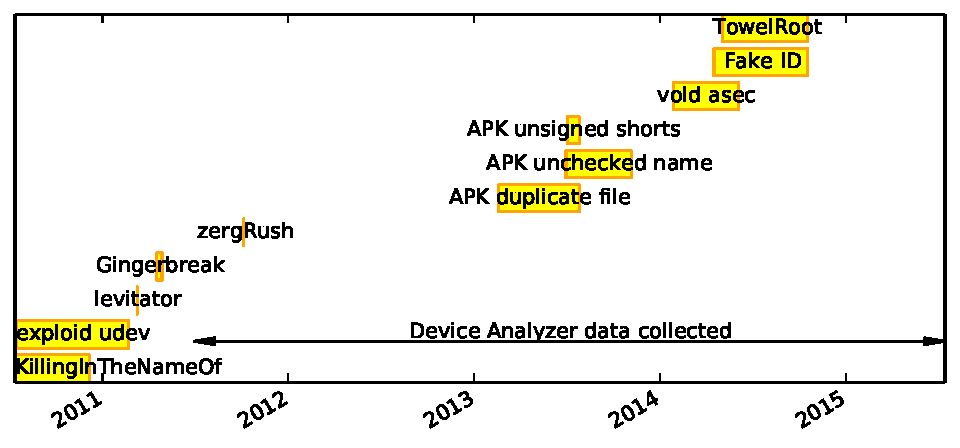
\includegraphics[width=\columnwidth]{figures/vulnerabilities_timeline}
 \caption{Timeline of vulnerabilities. For each vulnerability we show the dates of \textbf{discovery} and, when later, the dates of the first \textbf{fixing release}}
 \label{fig:vulnerabilities_timeline}
\end{figure}

Figure~\ref{fig:vulnerabilities_timeline} shows the dates of \textbf{discovery} and, when later, the date of the first \textbf{fixing release}.
Some vulnerabilities (\emph{levitator}, \emph{zergRush}) were fixed in released versions of Android before they were discovered and so are shown as vertical lines, while others were known for months before a version of Android which fixed them was shipped.
During the period in which \da\ data was collected the date when a version of Android with the fix was observed on a \da\ device is taken as the date that version was released.
For vulnerabilities prior to the collection period we estimate the release date as best we can using publicly available data.
There is no canonical source of Android release dates, and our best guesses and supporting references are available from \avo.

The discovery dates of our vulnerabilities does not appear to be uniform. 
In particular the data shows a large gap from 2011-10-06 to 2013-02-18 where we do not know of any discoveries of critical vulnerabilities affecting all Android devices.
The cause of this quiet period is unclear.
Possible explanations are that: (i) most devices were exposed to known vulnerabilities so there was no point in looking for new ones (from Figure~\ref{fig:proportioninsecure});
(ii) device manufacturers made it easier to install custom versions of Android, reducing the need for users to root their devices; and
(iii) device manufacturer specific vulnerabilities (which we are not in our analysis here) were easier to find and therefore attackers looking for vulnerabilities adjusted their focus.

\section{Android Ecosystem}\label{sec:android_ecosystem}
There is a complex Android ecosystem which creates and distributes updates to Android which fix vulnerabilities.
In this section we describe how the Android ecosystem functions and how Android versions, as seen by the \da\ project, are produced.


\subsection{Android update process}

\label{sec:android_update_process}
\begin{figure}
 \centering
 \def\svgwidth{\columnwidth}
 \import{figures/}{update_ecosystem.pdf_tex}
 \caption{Flow of updates between participants in the Android ecosystem.
 Numbers on edges indicate updates shipped between \daStartDate\ and \daEndDate, numbers in brackets represent number of such entities in our data.
 Dotted arrows indicate flows where we do not know how many updates are being produced as we can't measure those flows directly as they are not public.\todolater{Turn into a sankey diagram}}
 \label{fig:update_ecosystem}
\end{figure}
To understand how vulnerabilities in Android are fixed we must examine the Android update process which we model in Figure~\ref{fig:update_ecosystem}.
There are five entities or groups which contribute towards Android updates: the network operators, the device manufacturers, the hardware developers, Google and the upstream open source projects.
Android builds on various open source projects such as the Linux kernel, OpenSSL and BouncyCastle cryptography libraries.
Consequently Android can include any compatible versions of those projects, including those which fix security vulnerabilities.
Android also incorporates various drivers for different bits of hardware.
The Android platform is then built from these components by Google.
The code for each Android release or update is kept secret\footnote{\url{https://source.android.com/source/code-lines.html}} until after a binary release has been published.
Device manufacturers likely receive advanced access in order to prepare handsets so they can customise it before passing it on to the network operator.
The network operator may then make or request further customisations and perform further testing before shipping the update to the Device.
Sometimes device manufactures ship updates directly to the user, sometimes the device manufacturer and Google collaborate closely to make a particular phone, such as with Nexus devices.
Sometimes device manufacturers incorporate upstream open source project releases directly, and sometimes incorrectly -- for example previous work has recorded evidence of broken nightly builds of sqlite in Android releases~\cite{Wagner2013}.

The numbers of devices (\daNumOSDevices), network operators (\daNumOperators) and device manufacturers (\daNumManufacturers) in Figure~\ref{fig:update_ecosystem} come from the \da\ data.
Device manufacturer and network operator counts were obtained by normalising the results reported by Android to \da\ of the device manufacturer and active network operator.
This normalisation is a manual task involves removing invalid values (such as `manufacturer' or `airplane mode is on'), collating across company name changes (e.g.\ `lge' to `LG'), normalising punctuation, removing extra strings sometimes added such as (`(2g)' or `communications') and mapping some incorrectly placed model names back to their manufacturer.
This normalisation is not perfect and so these are overestimates on the \da\ data but they are likely still underestimates as there will be some device manufacturers and network operators which are not included in the \da\ data.

In Figure~\ref{fig:update_ecosystem} the number of updates received by devices (\daNumFullVersions) is the number of different full version strings observed in \da.
The number of updates shipped by Google (\daNumSigOSVersions) is the number of Android versions reported in \da\ which affected more than \daSigVersionPerc\ of devices for more than \daSigVersionDays\ days.
This significance test is to remove spurious versions recorded in \da\ such as `5.2.0' in 2012 which has still not been released in 2014.

We extracted data on the external projects used in Android and have included this and the scripts which generated it in \avo.
These scripts analysed the Android Open Source Project's source tree to examine the source code of each of the external projects to find the project version associated with each Android version tag on the repository.
There are \avoNumExternalProjects\ external open source projects in Android, contributing \avoTotalExternalLines\ lines of code.\footnote{Lines of code were measured using David A. Wheeler's \texttt{sloccount}.}
We analysed the top \avoNumBigExternalProjects\ by lines of code (\avoBigExternalLinesOfCodePerc\ of the total) and were able to automatically extract the versions of those projects included in different versions of Android for \avoNumAnalysedExternalProjects\ of these (\avoAnalysedExternalLinesOfCodePerc\ of the total).
We found \avoBigExternalTotalVersions\ distinct versions, a median of \avoBigExternalMedianVersions\ and mean of \avoBigExternalMeanVersions\ versions per project.
Android rarely changes the version of external projects it includes.

%An analysis by Vidas et al.~\cite{Vidas2011} of the Android 2.1 to 2.2 update found that it took 11 months from when Google released 2.2 for the last device which they were investigating to get the update.
To compute the latency between upstream releases and their inclusion in Android we scraped the release pages for those projects, to obtain the version numbers and release dates.
This allows us to compute the latency between an upstream project being released and it being included in Android, this is shown in Table~\ref{tab:update_ecosystem}.
The versions included in Android were about half a year old when the first version of Android containing it was released.
\begin{table}
\centering
\normalsize
\begin{tabular}{l|r|r}
Project	&	\# releases	&	latency (days) \\ \hline
linux	&	\linuxNumVersions	&	\linuxMeanUpdateLatency \\
openssl	&	\opensslNumVersions	&	\opensslMeanUpdateLatency \\
bouncycastle	&	\bouncycastleNumVersions	&	\bouncycastleMeanUpdateLatency \\
\end{tabular}
\caption{Flow of updates from upstream projects into Android. Number of updates as in Figure~\ref{fig:update_ecosystem}, latency in days for all pairs of versions we have data on.\todolater{scrape the other 26 websites... is it worth it?}}
\label{tab:update_ecosystem}
\end{table}






\section{Experiments}
\label{sec:results}
We present the results of our analysis showing that, on average, \daMeanInsecurityPerc\ of Android devices are exposed to critical vulnerabilities.
Devices, on average, apply \daUpdatesPerYear\ updates each year and \daPercUpdatesDowngrades\ of version changes are downgrades to older versions.
Nexus devices are better than others, \emph{\daSecScoreBestmanufacturer} is the highest scoring device manufacturer and \emph{\daSecScoreBestoperator} is the highest scoring network operator.
%\todo{comparison of nexus update rates with iOS}
We describe four experiments.
We examine the vulnerability of the Android ecosystem as a whole (\S\ref{sec:exp:versionsecurity}, explore the upgrade cycle and vulnerability cycle of the ecosystem (\S\ref{sec:exp:android_ecosystem}), quantify the updates installed on particular devices (\S\ref{sec:exp:device_updates}) and compare the performance of different device manufacturers and network operators (\S\ref{sec:exp:security_score}).

%% In an experiment you test a hypothesis, it needs to be clear what the hypothesis is and what the conclusion of the test is

\subsection{Experiment 0: vulnerability of Android devices}\label{sec:exp:versionsecurity}

In the introduction, Figure~\ref{fig:proportioninsecure} described the proportion of Android devices susceptable to at least one critical vulnerability.

\subsubsection{Method} 
To investigate the behaviour of the Android ecosystem as a whole with respect to Android versions and vulnerabilities we used the OS version information from \da\ and the vulnerability data from \avo.
The \da\ data used here was collected between \daStartDate\ and \daEndDate.
The \avo\ data covers the period from \avoFirstDataDate\ to \avoLastDataDate.
For each device we collected daily version data  and recorded the running version and any associated vulnerabilities it was exposed to at that time (if any).
We then normalise these totals for each day by dividing through by the total number of devices with version information seen on that day.

\subsubsection{Results}

Following time from left to right in Figure~\ref{fig:proportioninsecure} we see all devices are initially \emph{maybe secure} (yellow) since \da\ does not have historical data prior to May 2011. This means we cannot distinguish between devices which are running a version of Android which is known to be vulnerable from one which may have received a backported fix.
This demonstrates the importance of a longitudinal study: this type of analysis requires years of data.
Once \emph{zergRush} was discovered in October 2011 the most devices are recorded as \emph{insecure} (red) as most devices were exposed to that vulnerability.
The remanding devices were already running a version of Android which fixed the \emph{zergRush} vulnerability and are therefore marked as  \emph{secure} (green).
From October 2011 until the discovery of \emph{APK duplicate file} in February 2013 the graph shows progressive improvement as devices are upgraded. This means more and more devices are marked as \emph{secure} (green) because they are now running a secure version of Android, or marked as \emph{maybe secure} because they received a minor update which may have contained a backported fix.
From February 2013 onwards regular discovery of critical vulnerabilities ensures that most devices are exposed to known critical vulnerabilities.


\subsection{Experiment 1: behaviour of the Android ecosystem}\label{sec:exp:android_ecosystem}

\subsubsection{Method} As in Experiment 0, we used the version information for each device to calculate which critical vulnerabilities each device was susceptible to on a daily basis.

\subsubsection{Results}
The proportion of devices in the \da\ data running different versions of Android each day is shown in Figure~\ref{fig:norm_os}.
It shows how old versions are gradually replaced by new ones, and the long tail of devices which do not see updates to more recent versions.

\begin{figure*}
 \centering
 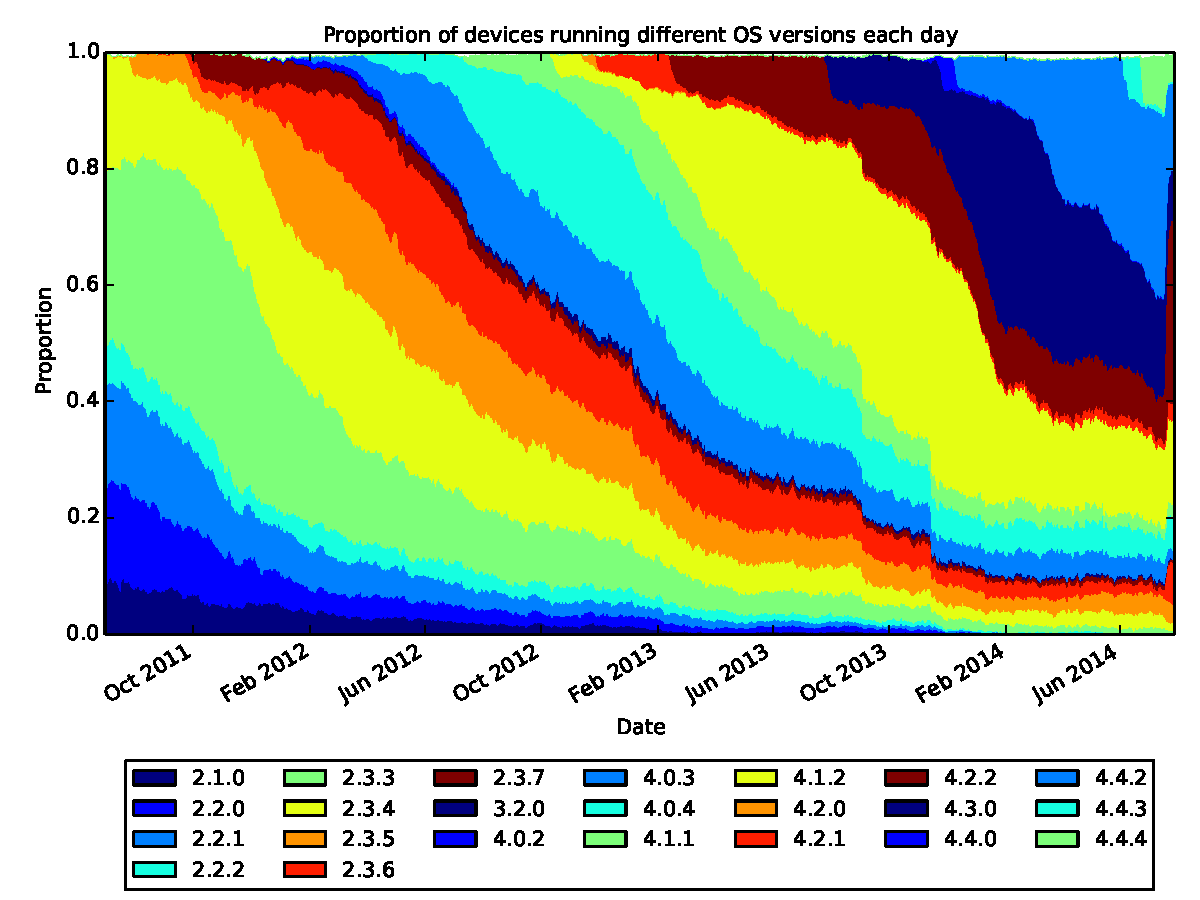
\includegraphics[width=\textwidth]{figures/da_norm_os}
 \caption{Android versions in \da\ data over time. The change in behaviour after August 2014 is explained in \S\ref{sec:da_changes}}
 \label{fig:norm_os}
\end{figure*}

The vulnerabilities devices are exposed to are shown in Figure~\ref{fig:nvulnerabilities_heat}.
For each vulnerability it shows the proportion of devices exposed to that vulnerability and how that changes over time.
The variation of the proportion of devices affected by a vulnerability with time tells us how badly a particular vulnerability affected the Android platform.
In July 2011 at the beginning of the \da\ data the \emph{exploid}\footnote{\url{http://androidvulnerabilities.org/vulnerabilities/exploid_udev}} and \emph{levitator}\footnote{\url{http://androidvulnerabilities.org/vulnerabilities/levitator}} vulnerabilities both affect most Android devices, slowly these are fixed as updates roll out and devices are replaced until in January 2013 a much smaller proportion of devices are affected by known vulnerabilities.
However when in February 2013 the first APK signing vulnerability was found which affected all previous versions of Android and even in October 2013 most devices (\daVulnAPKDuplicateFileOctoberPerc) were still vulnerable.
%\begin{figure}%[!b]
%\centering
%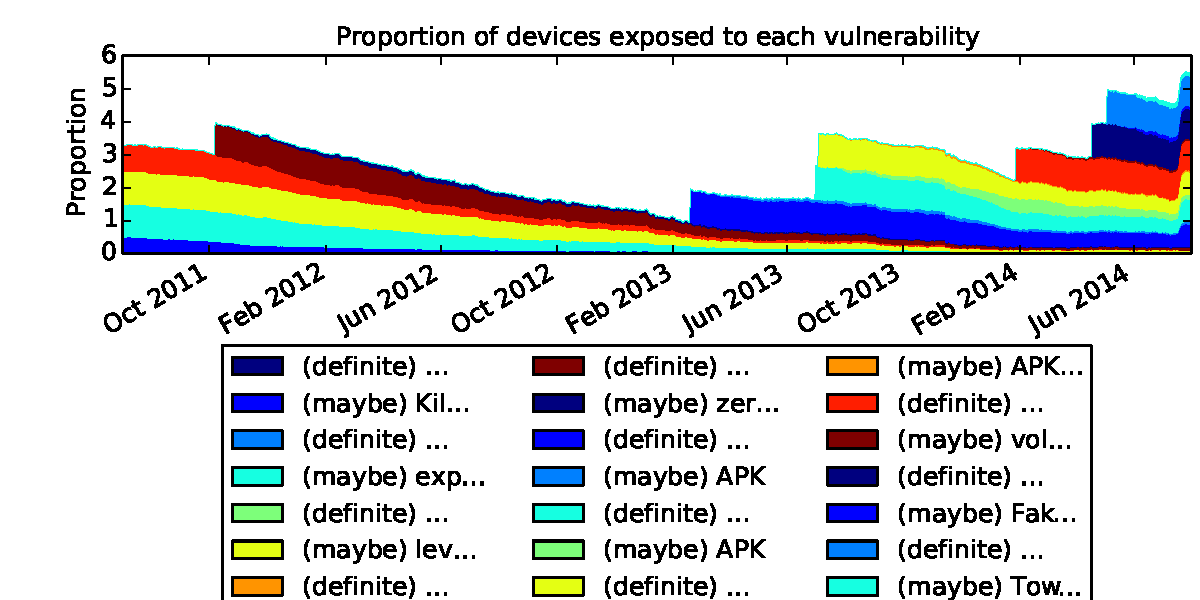
\includegraphics[width=\columnwidth]{figures/vulnerabilities}
%\caption{Proportion of devices exposed to each vulnerability with time (1.0 is 100\%)}
%\label{fig:vulnerabilities}
%\end{figure}

In 2013 three vulnerabilities were found in the way which Android verified the signatures on APKs.
These allowed the creation of malicious APKs which appear to be signed as system APKs -- which have root equivalent privileges.
Figure~\ref{fig:nvulnerabilities_heat} shows how the the \emph{APK signing vulnerabilities} affected all devices and took months to get fixed for any device.
However what is perhaps more worrying is the long tail on the \emph{Gingerbreak}\footnote{\url{http://androidvulnerabilities.org/vulnerabilities/Gingerbreak}}, \emph{levitator}, \emph{exploid} and \emph{zergRush}\footnote{\url{http://androidvulnerabilities.org/vulnerabilities/zergRush}} vulnerabilities which are more dangerous root vulnerabilities (not requiring new APK installation) and which still affect a significant proportion of devices years later.


\begin{figure*}
 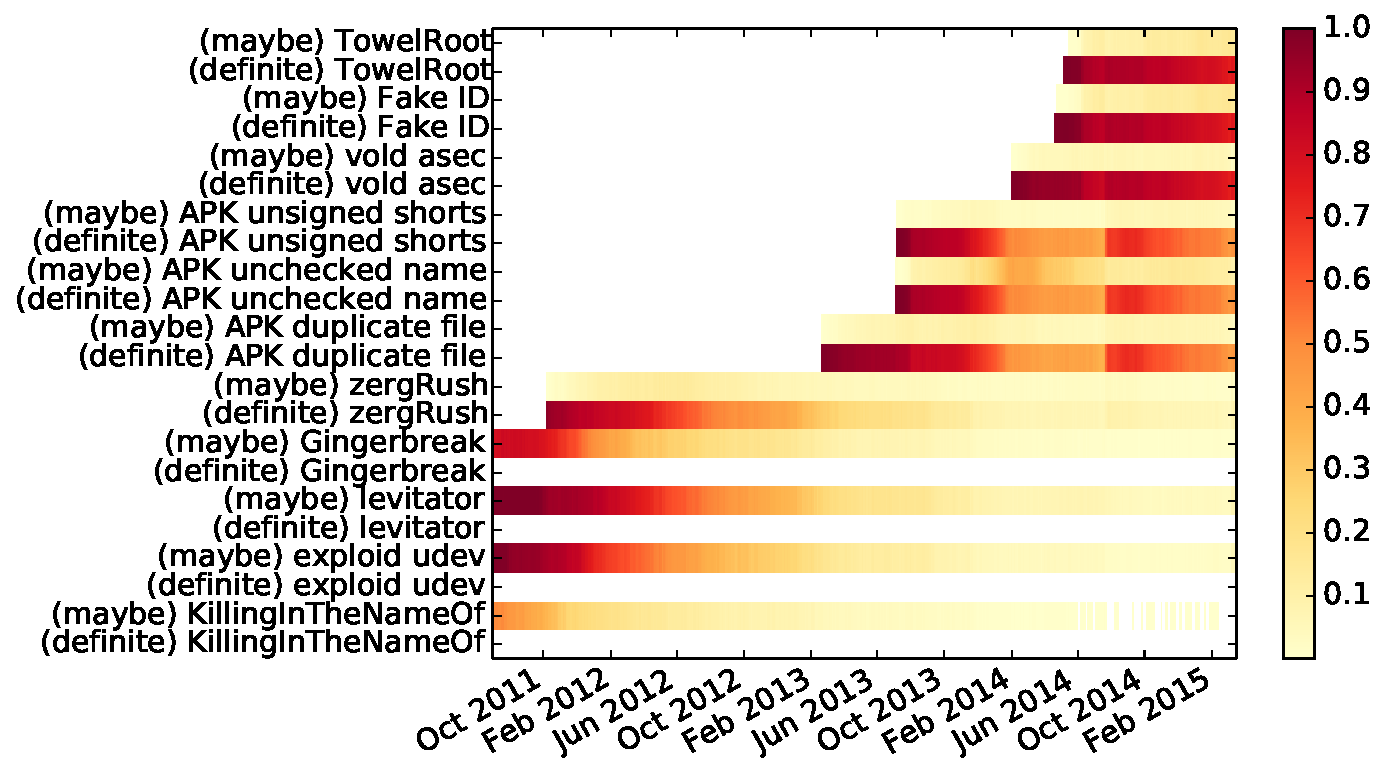
\includegraphics[width=\textwidth]{figures/nvulnerabilities_heat.pdf}
 \caption{Proportion of devices affected by different vulnerabilities. The prefix `(maybe)' indicates `maybe insecure' and `(definite)' indicates `definitely insecure'. The first few vulnerabilities are all `maybe insecure' as we do not have data from before that vulnerability was discovered while later ones are mostly `definitely insecure' as we know no fixing update reached the devices. The change in behaviour after August 2014 is explained in \S\ref{sec:da_changes}}
 \label{fig:nvulnerabilities_heat}
\end{figure*}


\subsection{Experiment 2: Updates to particular devices}\label{sec:exp:device_updates}
Those graphs summarise data across all the devices, however one of the advantages of the \da\ data is that it allows us to look at what happens to individual devices over time.

\subsubsection{Method}
As in Experiment 0, we used the version information for each device to calculate which critical vulnerabilities each device was susceptible to on a daily basis.
We also recorded when the version changed and which versions it changed from and to.
In the \da\ data we have over 1000 devices contributing data in any particular week.
However most devices only contribute for a short period of time and so we do not observe updates happening on every device.
Instead we have a hopefully representative sample of upgrades which happened while \da\ was installed on the devices.
\da\ cannot distinguish between a device being replaced and the \da\ app being removed as while multiple devices can be linked to the same user account, that is a manual process and few users do it.


\subsubsection{Results}
\begin{figure}
 \centering
 \begin{subfigure}[b]{\columnwidth}
  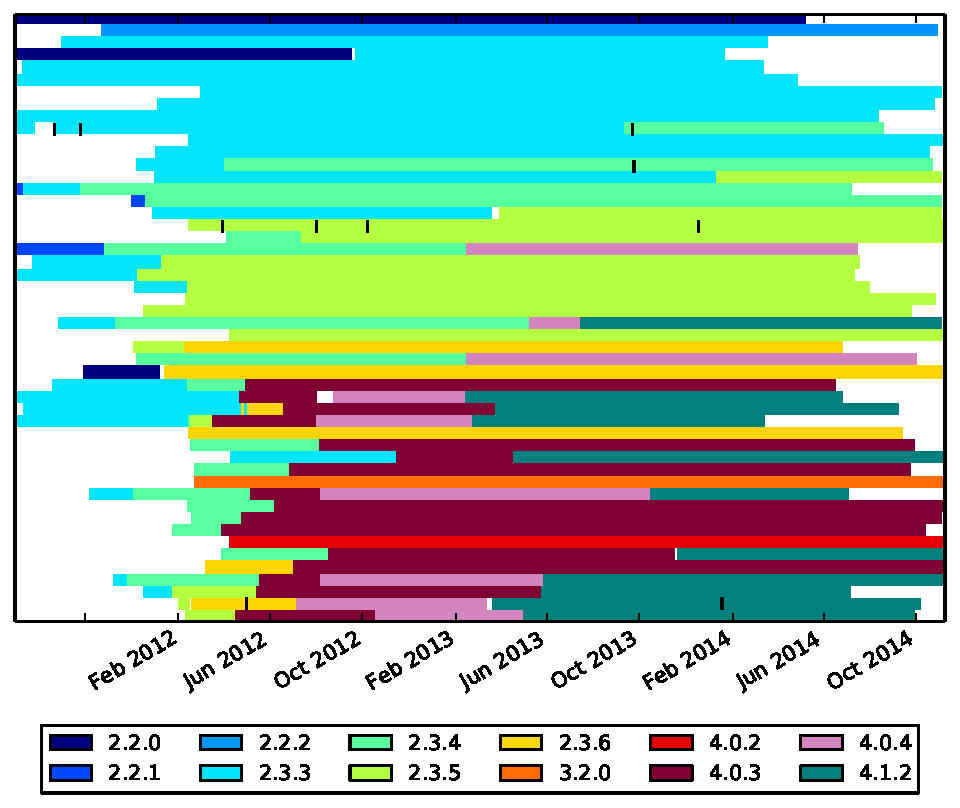
\includegraphics[width=\columnwidth]{figures/device-data-all-os}
  \caption{OS versions over time. Black vertical lines indicate that the build number changed without changing the OS version at that point.}
  \label{fig:device_data_os}
 \end{subfigure}
 \begin{subfigure}[b]{\columnwidth}
  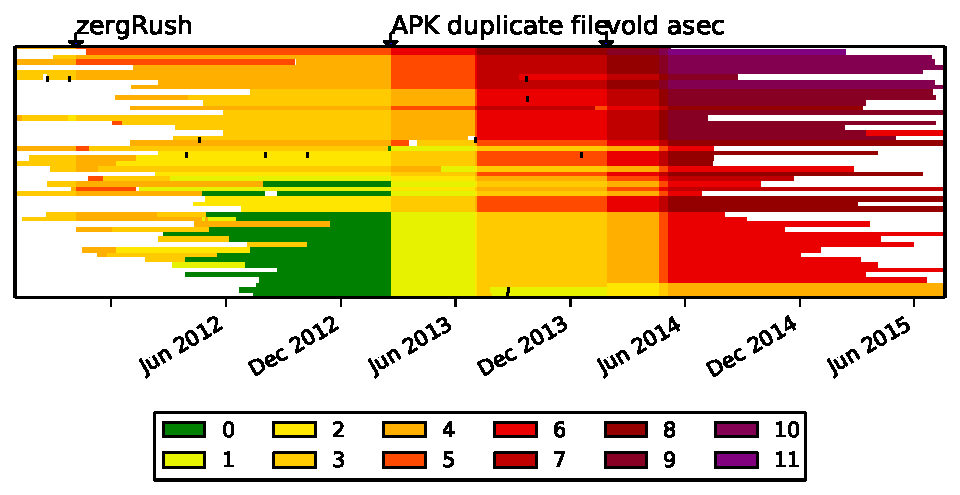
\includegraphics[width=\columnwidth]{figures/device-data-all-security}
  \caption{Number of vulnerabilities affecting each device over time}
  \label{fig:device_data_security}
 \end{subfigure}
 \caption{The top \daNumDeviceDataDevices\ devices by days of contribution in the \da\ data. One strip per device handset.}
\end{figure}
The longitudinal data on the number of vulnerabilities affecting the \daNumDeviceDataDevices\ devices which have contributed the most days of data to \da\ changes over time is shown in Figure~\ref{fig:device_data_security}.
The trend that we saw in Figure~\ref{fig:proportioninsecure} of security improving and then getting worse is also shown here.
It shows how some devices had vulnerabilities, which were fixed, and then further vulnerabilities were discovered, and for these devices, mostly not fixed.
This implies that these devices had been abandoned by the device manufacturer and were not receiving updates which is confirmed by Figure~\ref{fig:device_data_os} which shows which OS versions those devices were running.
Some devices start off in 2011 exposed to known security vulnerabilities and are still exposed to those and additional ones in 2014.


\begin{figure}
 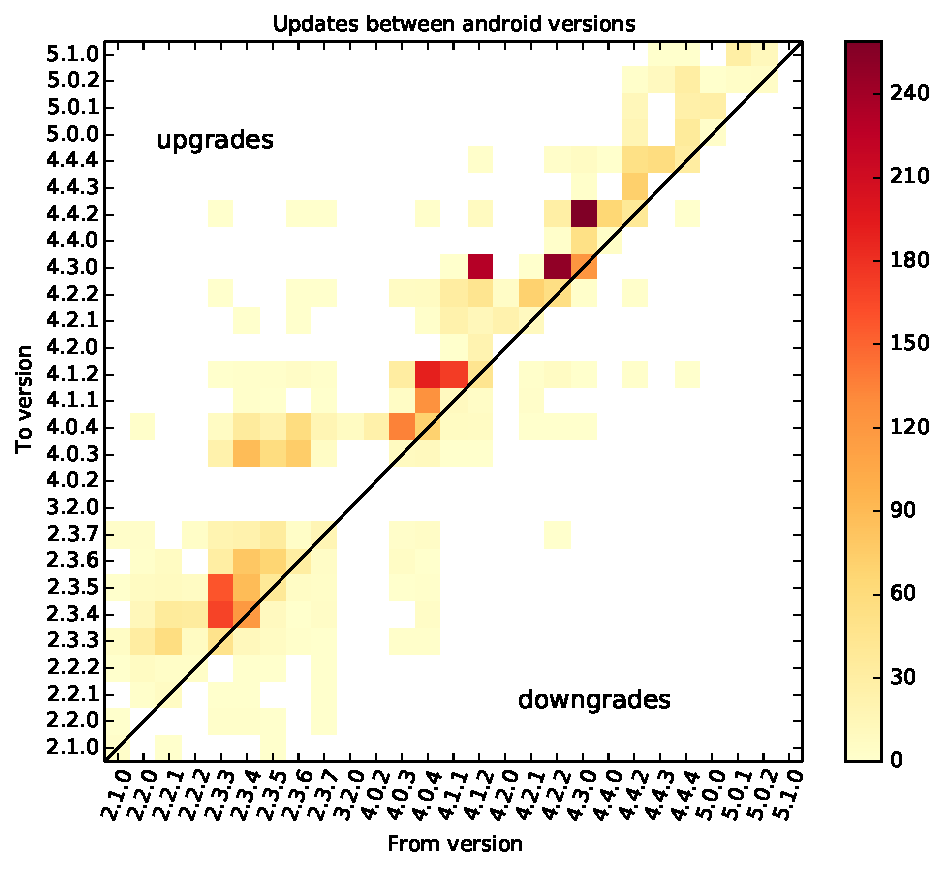
\includegraphics[width=\columnwidth]{figures/from_to_updates.pdf}
 \caption{Updates between different Android versions in the \da\ data}
 \label{fig:from_to_updates}
\end{figure}
\begin{figure}
 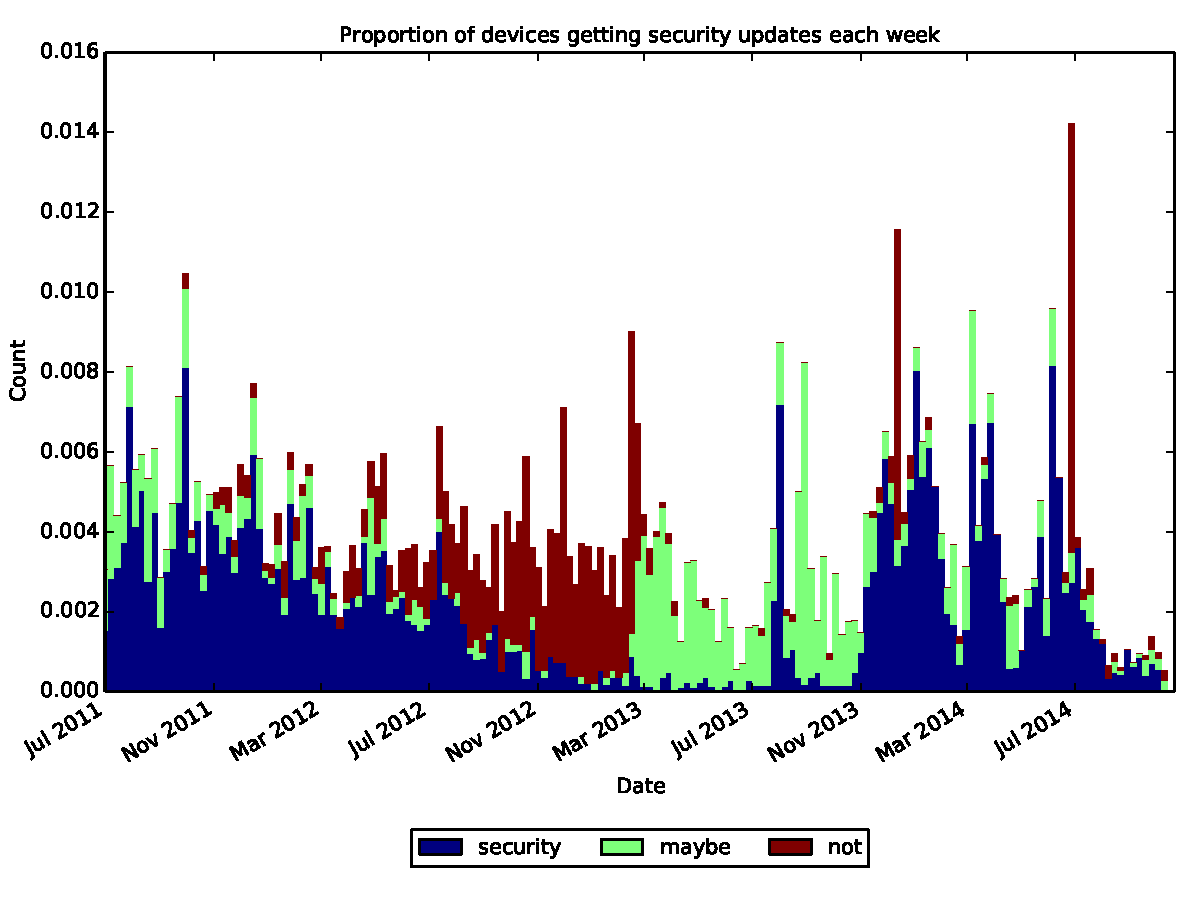
\includegraphics[width=\columnwidth]{figures/nw_security_updates.pdf}
 \caption{Proportion of updates each week which fixed or may have fixed security vulnerabilities}
 \label{fig:weekly_security_updates}
\end{figure}
We recorded update events and Figure~\ref{fig:from_to_updates} shows how devices upgrade between different versions of Android.
Mostly the dark cells are upgrades (above the diagonal) (\daNumUpdatesUpgrades).
While many upgrades are from one version to the next version there are also a fair number (\daNumUpdatesBigUpgrades, \daPercBigUpgrades) which skip more than \daNumUpdatesSkippedBig\ versions.
Surprisingly there are also a small number of downgrade events (\daNumUpdatesDowngrades, \daPercUpdatesDowngrades) when older versions of Android are installed on to devices.
Possible reasons why users are downgrading are to free up space on their device, to make it easier to root or because a new version introduced bugs.

The number of devices getting security updates each week, is shown in Figure~\ref{fig:weekly_security_updates}.
\begin{itemize}
 \item Updates which changed the Android version number from a version with known vulnerabilities to one which had fewer known vulnerabilities are shown in red.
 \item Updates which changed the build number but not the version number and so might contain a backported fix for a vulnerability are shown in yellow.
\item Updates which did not fix security vulnerabilities (because there were no known security vulnerabilities in the version of Android they were already running) are shown in green.

\end{itemize}

By taking the number of updates observed and the number of device days of data we have collected we can compute the number of updates received by a device per year to be \daUpdatesPerYear.
This compares badly with the number of critical vulnerabilities discovered per year of between \avoVulnsPerYearAllAndroid\ (affecting all Android) and \avoVulnsPerYear\ (including the device manufacturer specific ones in \avo).


\section{Comparing device manufacturers, device models and network operators}
\label{sec:security_scoring}\label{sec:exp:security_score}

To allow buyers of Android devices to purchase those devices which have the best security they need to know how different device manufacturers, device models and network operators compare in terms of the security they provide.
We propose a method to score a device manufacturer, device model or network operator based on its historic performance at keeping devices up-to-date and fixing security vulnerabilities.
We find that Android as a whole gets a score of \daSecurityScore\ out of 10, the highest scoring device manufacturer is \emph{\daSecScoreBestmanufacturer} (\daSecScoreBestmanufacturerScore\ out of 10) and the lowest scoring is \emph{\daSecScoreWorstmanufacturer} (\daSecScoreWorstmanufacturerScore\ out of 10).

\subsection{Method: Scoring for security}\label{sec:security_scoring:method}

Computing how good a particular device manufacturer or device model is from a security standpoint is difficult as it depends on a number of factors which are hard to observe, particularly on a large scale.
Ideally we would consider both the prevalence of potential problems which were not exploited and actual security failures.
%\footnote{A perfectly secure operating system would among other things detect and prevent all phishing attacks, provide perfect principle of least privilege isolation, not have any vulnerabilities, instantly fix all discovered vulnerabilities, not allow any user data to be used in a way which the user does not approve of and be really easy for an ordinary person to use.}
However in the absence of such data we propose a scheme for assigning a device a score out of ten based on data which can be observed, is based on previous metrics, and which we expect correlates with the actual security of the devices.

The FUM score is computed from three components:
\begin{description}
  \item[free $f$] The proportion of running devices which were free from critical vulnerabilities over time. This is equivalent to Acer and Jackson's proposal to measure the security based on the proportion of users with at least one unpatched critical vulnerability~\cite{Acer2010} and similar to the Vulnerability Free Days (VFD) score~\cite{Wright2014}.
  Unlike VFD this is the proportion of running devices which were free from critical vulnerabilities over time, rather than days which the device manufacturer was free from outstanding critical vulnerabilities as that does not take account of the update process.
  \item[update $u$] The proportion of devices which run the latest version of Android shipped to any device produced by that device manufacturer. This is a measure of internal updatedness, a low score would mean many devices are being left behind.
  This assumes that newer versions are better with stronger security.
  Historically steps have been taken to improve Android security in newer versions so this assumption should generally hold, but sometimes new updates introduce new vulnerabilities.
  \item[mean $m$] The mean number of outstanding vulnerabilities affecting devices not fixed on any device shipped by the device manufacturer. This is related to the Median Active Vulnerabilities (MAV) measure~\cite{Wright2014} but is the mean rather than the median, as this gives a continuous value.
  An example is given in Figure~\ref{fig:mcalculation}.
%TODO should we compute the median instead?
\end{description}

\begin{figure}
\centering
%\includegraphics[width=\columnwidth]{figures/mcalculation}
% Graphic for TeX using PGF
% Title: /home/drt24/git/papers/da/securityupdates/figures/mcalculation.dia
% Creator: Dia v0.97.3
% CreationDate: Wed Apr 22 15:03:07 2015
% For: drt24
% \usepackage{tikz}
% The following commands are not supported in PSTricks at present
% We define them conditionally, so when they are implemented,
% this pgf file will use them.
\ifx\du\undefined
  \newlength{\du}
\fi
\setlength{\du}{5\unitlength}
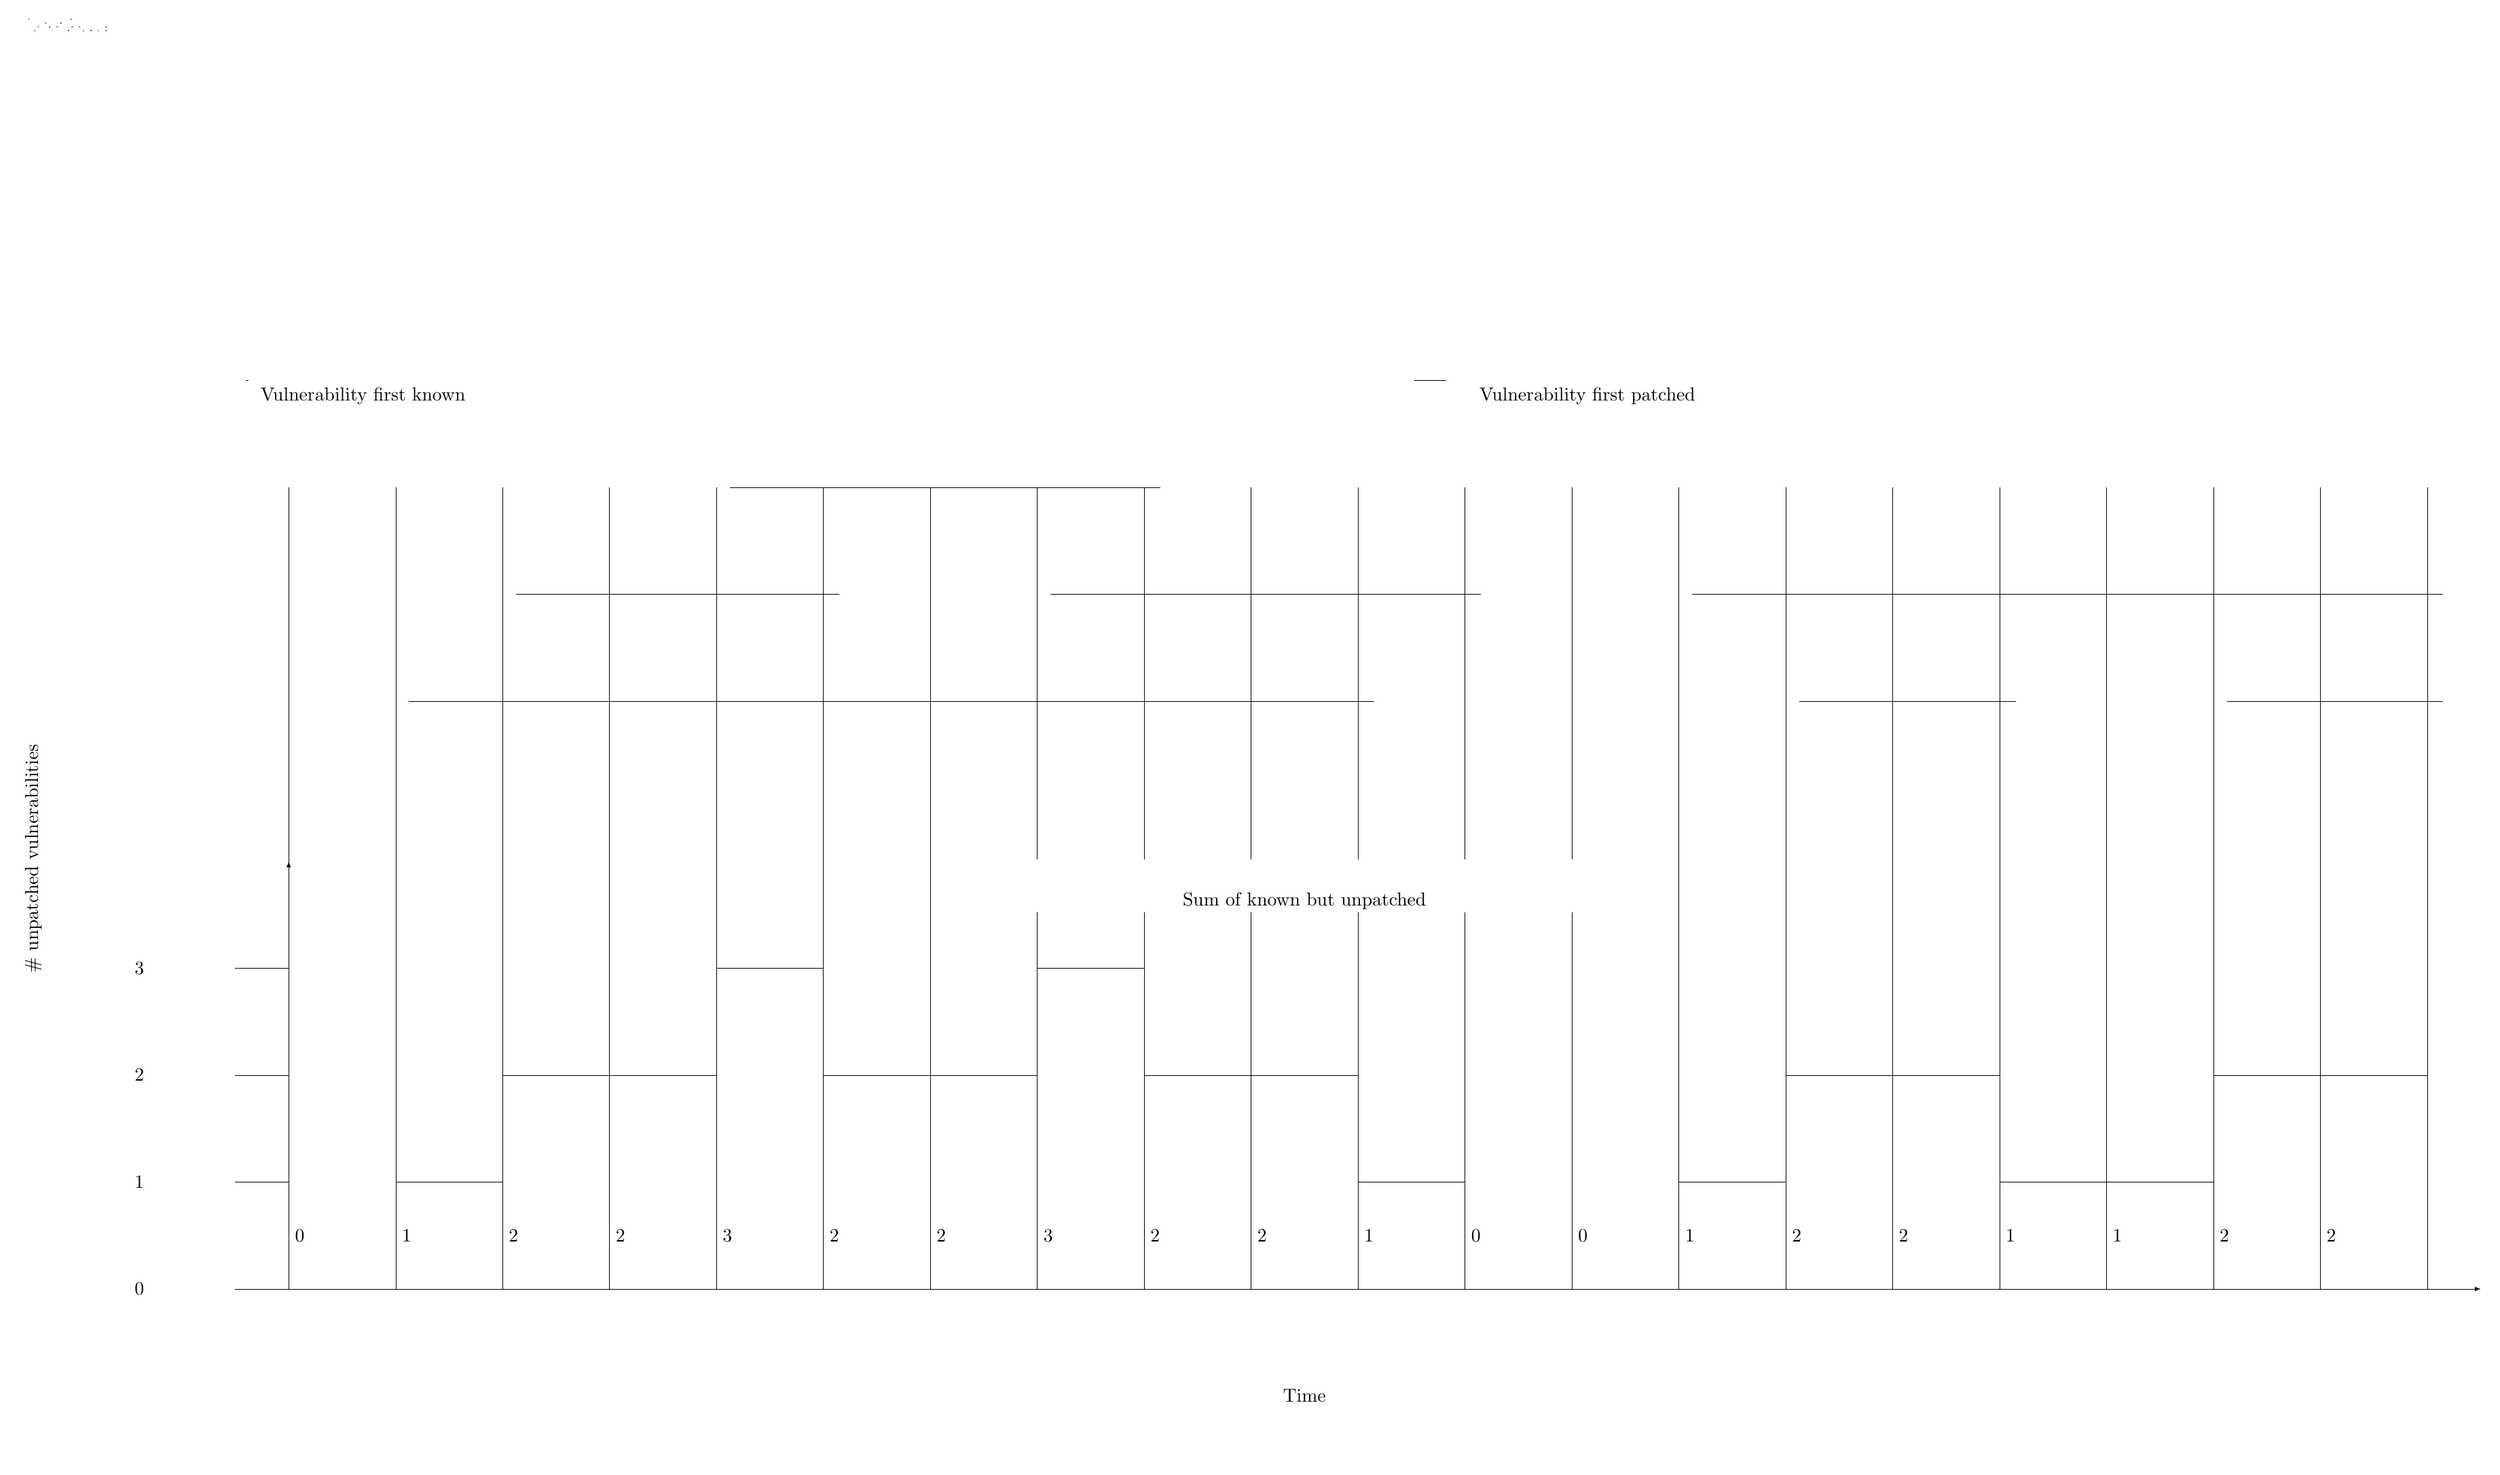
\begin{tikzpicture}
\pgftransformxscale{1.000000}
\pgftransformyscale{-1.000000}
\definecolor{dialinecolor}{rgb}{0.000000, 0.000000, 0.000000}
\pgfsetstrokecolor{dialinecolor}
\definecolor{dialinecolor}{rgb}{1.000000, 1.000000, 1.000000}
\pgfsetfillcolor{dialinecolor}
\pgfsetlinewidth{0.100000\du}
\pgfsetdash{{\pgflinewidth}{0.200000\du}}{0cm}
\pgfsetdash{{\pgflinewidth}{0.200000\du}}{0cm}
\pgfsetbuttcap
{
\definecolor{dialinecolor}{rgb}{0.000000, 0.000000, 0.000000}
\pgfsetfillcolor{dialinecolor}
% was here!!!
\definecolor{dialinecolor}{rgb}{0.000000, 0.000000, 0.000000}
\pgfsetstrokecolor{dialinecolor}
\draw (5.000000\du,24.000000\du)--(5.000000\du,9.000000\du);
}
\pgfsetlinewidth{0.100000\du}
\pgfsetdash{{\pgflinewidth}{0.200000\du}}{0cm}
\pgfsetdash{{\pgflinewidth}{0.200000\du}}{0cm}
\pgfsetbuttcap
{
\definecolor{dialinecolor}{rgb}{0.000000, 0.000000, 0.000000}
\pgfsetfillcolor{dialinecolor}
% was here!!!
\definecolor{dialinecolor}{rgb}{0.000000, 0.000000, 0.000000}
\pgfsetstrokecolor{dialinecolor}
\draw (7.000000\du,24.000000\du)--(7.000000\du,9.000000\du);
}
\pgfsetlinewidth{0.100000\du}
\pgfsetdash{{\pgflinewidth}{0.200000\du}}{0cm}
\pgfsetdash{{\pgflinewidth}{0.200000\du}}{0cm}
\pgfsetbuttcap
{
\definecolor{dialinecolor}{rgb}{0.000000, 0.000000, 0.000000}
\pgfsetfillcolor{dialinecolor}
% was here!!!
\definecolor{dialinecolor}{rgb}{0.000000, 0.000000, 0.000000}
\pgfsetstrokecolor{dialinecolor}
\draw (9.000000\du,24.000000\du)--(9.000000\du,9.000000\du);
}
\pgfsetlinewidth{0.100000\du}
\pgfsetdash{{\pgflinewidth}{0.200000\du}}{0cm}
\pgfsetdash{{\pgflinewidth}{0.200000\du}}{0cm}
\pgfsetbuttcap
{
\definecolor{dialinecolor}{rgb}{0.000000, 0.000000, 0.000000}
\pgfsetfillcolor{dialinecolor}
% was here!!!
\definecolor{dialinecolor}{rgb}{0.000000, 0.000000, 0.000000}
\pgfsetstrokecolor{dialinecolor}
\draw (11.000000\du,24.000000\du)--(11.000000\du,9.000000\du);
}
\pgfsetlinewidth{0.100000\du}
\pgfsetdash{{\pgflinewidth}{0.200000\du}}{0cm}
\pgfsetdash{{\pgflinewidth}{0.200000\du}}{0cm}
\pgfsetbuttcap
{
\definecolor{dialinecolor}{rgb}{0.000000, 0.000000, 0.000000}
\pgfsetfillcolor{dialinecolor}
% was here!!!
\definecolor{dialinecolor}{rgb}{0.000000, 0.000000, 0.000000}
\pgfsetstrokecolor{dialinecolor}
\draw (13.000000\du,24.000000\du)--(13.000000\du,9.000000\du);
}
\pgfsetlinewidth{0.100000\du}
\pgfsetdash{{\pgflinewidth}{0.200000\du}}{0cm}
\pgfsetdash{{\pgflinewidth}{0.200000\du}}{0cm}
\pgfsetbuttcap
{
\definecolor{dialinecolor}{rgb}{0.000000, 0.000000, 0.000000}
\pgfsetfillcolor{dialinecolor}
% was here!!!
\definecolor{dialinecolor}{rgb}{0.000000, 0.000000, 0.000000}
\pgfsetstrokecolor{dialinecolor}
\draw (15.000000\du,24.000000\du)--(15.000000\du,9.000000\du);
}
\pgfsetlinewidth{0.100000\du}
\pgfsetdash{{\pgflinewidth}{0.200000\du}}{0cm}
\pgfsetdash{{\pgflinewidth}{0.200000\du}}{0cm}
\pgfsetbuttcap
{
\definecolor{dialinecolor}{rgb}{0.000000, 0.000000, 0.000000}
\pgfsetfillcolor{dialinecolor}
% was here!!!
\definecolor{dialinecolor}{rgb}{0.000000, 0.000000, 0.000000}
\pgfsetstrokecolor{dialinecolor}
\draw (17.000000\du,24.000000\du)--(17.000000\du,9.000000\du);
}
\pgfsetlinewidth{0.100000\du}
\pgfsetdash{{\pgflinewidth}{0.200000\du}}{0cm}
\pgfsetdash{{\pgflinewidth}{0.200000\du}}{0cm}
\pgfsetbuttcap
{
\definecolor{dialinecolor}{rgb}{0.000000, 0.000000, 0.000000}
\pgfsetfillcolor{dialinecolor}
% was here!!!
\definecolor{dialinecolor}{rgb}{0.000000, 0.000000, 0.000000}
\pgfsetstrokecolor{dialinecolor}
\draw (19.000000\du,24.000000\du)--(19.000000\du,9.000000\du);
}
\pgfsetlinewidth{0.100000\du}
\pgfsetdash{{\pgflinewidth}{0.200000\du}}{0cm}
\pgfsetdash{{\pgflinewidth}{0.200000\du}}{0cm}
\pgfsetbuttcap
{
\definecolor{dialinecolor}{rgb}{0.000000, 0.000000, 0.000000}
\pgfsetfillcolor{dialinecolor}
% was here!!!
\definecolor{dialinecolor}{rgb}{0.000000, 0.000000, 0.000000}
\pgfsetstrokecolor{dialinecolor}
\draw (21.000000\du,24.000000\du)--(21.000000\du,9.000000\du);
}
\pgfsetlinewidth{0.100000\du}
\pgfsetdash{{\pgflinewidth}{0.200000\du}}{0cm}
\pgfsetdash{{\pgflinewidth}{0.200000\du}}{0cm}
\pgfsetbuttcap
{
\definecolor{dialinecolor}{rgb}{0.000000, 0.000000, 0.000000}
\pgfsetfillcolor{dialinecolor}
% was here!!!
\definecolor{dialinecolor}{rgb}{0.000000, 0.000000, 0.000000}
\pgfsetstrokecolor{dialinecolor}
\draw (23.000000\du,24.000000\du)--(23.000000\du,9.000000\du);
}
\pgfsetlinewidth{0.100000\du}
\pgfsetdash{{\pgflinewidth}{0.200000\du}}{0cm}
\pgfsetdash{{\pgflinewidth}{0.200000\du}}{0cm}
\pgfsetbuttcap
{
\definecolor{dialinecolor}{rgb}{0.000000, 0.000000, 0.000000}
\pgfsetfillcolor{dialinecolor}
% was here!!!
\definecolor{dialinecolor}{rgb}{0.000000, 0.000000, 0.000000}
\pgfsetstrokecolor{dialinecolor}
\draw (25.000000\du,24.000000\du)--(25.000000\du,9.000000\du);
}
\pgfsetlinewidth{0.100000\du}
\pgfsetdash{{\pgflinewidth}{0.200000\du}}{0cm}
\pgfsetdash{{\pgflinewidth}{0.200000\du}}{0cm}
\pgfsetbuttcap
{
\definecolor{dialinecolor}{rgb}{0.000000, 0.000000, 0.000000}
\pgfsetfillcolor{dialinecolor}
% was here!!!
\definecolor{dialinecolor}{rgb}{0.000000, 0.000000, 0.000000}
\pgfsetstrokecolor{dialinecolor}
\draw (27.000000\du,24.000000\du)--(27.000000\du,9.000000\du);
}
\pgfsetlinewidth{0.100000\du}
\pgfsetdash{{\pgflinewidth}{0.200000\du}}{0cm}
\pgfsetdash{{\pgflinewidth}{0.200000\du}}{0cm}
\pgfsetbuttcap
{
\definecolor{dialinecolor}{rgb}{0.000000, 0.000000, 0.000000}
\pgfsetfillcolor{dialinecolor}
% was here!!!
\definecolor{dialinecolor}{rgb}{0.000000, 0.000000, 0.000000}
\pgfsetstrokecolor{dialinecolor}
\draw (29.000000\du,24.000000\du)--(29.000000\du,9.000000\du);
}
\pgfsetlinewidth{0.100000\du}
\pgfsetdash{{\pgflinewidth}{0.200000\du}}{0cm}
\pgfsetdash{{\pgflinewidth}{0.200000\du}}{0cm}
\pgfsetbuttcap
{
\definecolor{dialinecolor}{rgb}{0.000000, 0.000000, 0.000000}
\pgfsetfillcolor{dialinecolor}
% was here!!!
\definecolor{dialinecolor}{rgb}{0.000000, 0.000000, 0.000000}
\pgfsetstrokecolor{dialinecolor}
\draw (31.000000\du,24.000000\du)--(31.000000\du,9.000000\du);
}
\pgfsetlinewidth{0.100000\du}
\pgfsetdash{}{0pt}
\pgfsetdash{}{0pt}
\pgfsetbuttcap
{
\definecolor{dialinecolor}{rgb}{0.000000, 0.000000, 0.000000}
\pgfsetfillcolor{dialinecolor}
% was here!!!
\pgfsetarrowsend{latex}
\definecolor{dialinecolor}{rgb}{0.000000, 0.000000, 0.000000}
\pgfsetstrokecolor{dialinecolor}
\draw (5.000000\du,24.000000\du)--(46.000000\du,24.000000\du);
}
\pgfsetlinewidth{0.100000\du}
\pgfsetdash{}{0pt}
\pgfsetdash{}{0pt}
\pgfsetbuttcap
{
\definecolor{dialinecolor}{rgb}{0.000000, 0.000000, 0.000000}
\pgfsetfillcolor{dialinecolor}
% was here!!!
}
\definecolor{dialinecolor}{rgb}{0.000000, 0.000000, 0.000000}
\pgfsetstrokecolor{dialinecolor}
\draw (7.250000\du,13.000000\du)--(25.300000\du,13.000000\du);
\pgfsetlinewidth{0.100000\du}
\pgfsetdash{}{0pt}
\pgfsetmiterjoin
\pgfsetbuttcap
\definecolor{dialinecolor}{rgb}{1.000000, 1.000000, 1.000000}
\pgfsetfillcolor{dialinecolor}
\pgfpathmoveto{\pgfpoint{6.750000\du}{13.000000\du}}
\pgfpathcurveto{\pgfpoint{6.750000\du}{12.875000\du}}{\pgfpoint{6.875000\du}{12.750000\du}}{\pgfpoint{7.000000\du}{12.750000\du}}
\pgfpathcurveto{\pgfpoint{7.125000\du}{12.750000\du}}{\pgfpoint{7.250000\du}{12.875000\du}}{\pgfpoint{7.250000\du}{13.000000\du}}
\pgfpathcurveto{\pgfpoint{7.250000\du}{13.125000\du}}{\pgfpoint{7.125000\du}{13.250000\du}}{\pgfpoint{7.000000\du}{13.250000\du}}
\pgfpathcurveto{\pgfpoint{6.875000\du}{13.250000\du}}{\pgfpoint{6.750000\du}{13.125000\du}}{\pgfpoint{6.750000\du}{13.000000\du}}
\pgfusepath{fill}
\definecolor{dialinecolor}{rgb}{0.000000, 0.000000, 0.000000}
\pgfsetstrokecolor{dialinecolor}
\pgfpathmoveto{\pgfpoint{6.750000\du}{13.000000\du}}
\pgfpathcurveto{\pgfpoint{6.750000\du}{12.875000\du}}{\pgfpoint{6.875000\du}{12.750000\du}}{\pgfpoint{7.000000\du}{12.750000\du}}
\pgfpathcurveto{\pgfpoint{7.125000\du}{12.750000\du}}{\pgfpoint{7.250000\du}{12.875000\du}}{\pgfpoint{7.250000\du}{13.000000\du}}
\pgfpathcurveto{\pgfpoint{7.250000\du}{13.125000\du}}{\pgfpoint{7.125000\du}{13.250000\du}}{\pgfpoint{7.000000\du}{13.250000\du}}
\pgfpathcurveto{\pgfpoint{6.875000\du}{13.250000\du}}{\pgfpoint{6.750000\du}{13.125000\du}}{\pgfpoint{6.750000\du}{13.000000\du}}
\pgfusepath{stroke}
\pgfsetlinewidth{0.100000\du}
\pgfsetdash{}{0pt}
\pgfsetmiterjoin
\pgfsetbuttcap
\definecolor{dialinecolor}{rgb}{0.000000, 0.000000, 0.000000}
\pgfsetfillcolor{dialinecolor}
\pgfpathmoveto{\pgfpoint{25.300000\du}{13.000000\du}}
\pgfpathcurveto{\pgfpoint{25.300000\du}{13.125000\du}}{\pgfpoint{25.175000\du}{13.250000\du}}{\pgfpoint{25.050000\du}{13.250000\du}}
\pgfpathcurveto{\pgfpoint{24.925000\du}{13.250000\du}}{\pgfpoint{24.800000\du}{13.125000\du}}{\pgfpoint{24.800000\du}{13.000000\du}}
\pgfpathcurveto{\pgfpoint{24.800000\du}{12.875000\du}}{\pgfpoint{24.925000\du}{12.750000\du}}{\pgfpoint{25.050000\du}{12.750000\du}}
\pgfpathcurveto{\pgfpoint{25.175000\du}{12.750000\du}}{\pgfpoint{25.300000\du}{12.875000\du}}{\pgfpoint{25.300000\du}{13.000000\du}}
\pgfusepath{fill}
\definecolor{dialinecolor}{rgb}{0.000000, 0.000000, 0.000000}
\pgfsetstrokecolor{dialinecolor}
\pgfpathmoveto{\pgfpoint{25.300000\du}{13.000000\du}}
\pgfpathcurveto{\pgfpoint{25.300000\du}{13.125000\du}}{\pgfpoint{25.175000\du}{13.250000\du}}{\pgfpoint{25.050000\du}{13.250000\du}}
\pgfpathcurveto{\pgfpoint{24.925000\du}{13.250000\du}}{\pgfpoint{24.800000\du}{13.125000\du}}{\pgfpoint{24.800000\du}{13.000000\du}}
\pgfpathcurveto{\pgfpoint{24.800000\du}{12.875000\du}}{\pgfpoint{24.925000\du}{12.750000\du}}{\pgfpoint{25.050000\du}{12.750000\du}}
\pgfpathcurveto{\pgfpoint{25.175000\du}{12.750000\du}}{\pgfpoint{25.300000\du}{12.875000\du}}{\pgfpoint{25.300000\du}{13.000000\du}}
\pgfusepath{stroke}
\pgfsetlinewidth{0.100000\du}
\pgfsetdash{}{0pt}
\pgfsetdash{}{0pt}
\pgfsetbuttcap
{
\definecolor{dialinecolor}{rgb}{0.000000, 0.000000, 0.000000}
\pgfsetfillcolor{dialinecolor}
% was here!!!
}
\definecolor{dialinecolor}{rgb}{0.000000, 0.000000, 0.000000}
\pgfsetstrokecolor{dialinecolor}
\draw (9.250000\du,11.000000\du)--(15.300000\du,11.000000\du);
\pgfsetlinewidth{0.100000\du}
\pgfsetdash{}{0pt}
\pgfsetmiterjoin
\pgfsetbuttcap
\definecolor{dialinecolor}{rgb}{1.000000, 1.000000, 1.000000}
\pgfsetfillcolor{dialinecolor}
\pgfpathmoveto{\pgfpoint{8.750000\du}{11.000000\du}}
\pgfpathcurveto{\pgfpoint{8.750000\du}{10.875000\du}}{\pgfpoint{8.875000\du}{10.750000\du}}{\pgfpoint{9.000000\du}{10.750000\du}}
\pgfpathcurveto{\pgfpoint{9.125000\du}{10.750000\du}}{\pgfpoint{9.250000\du}{10.875000\du}}{\pgfpoint{9.250000\du}{11.000000\du}}
\pgfpathcurveto{\pgfpoint{9.250000\du}{11.125000\du}}{\pgfpoint{9.125000\du}{11.250000\du}}{\pgfpoint{9.000000\du}{11.250000\du}}
\pgfpathcurveto{\pgfpoint{8.875000\du}{11.250000\du}}{\pgfpoint{8.750000\du}{11.125000\du}}{\pgfpoint{8.750000\du}{11.000000\du}}
\pgfusepath{fill}
\definecolor{dialinecolor}{rgb}{0.000000, 0.000000, 0.000000}
\pgfsetstrokecolor{dialinecolor}
\pgfpathmoveto{\pgfpoint{8.750000\du}{11.000000\du}}
\pgfpathcurveto{\pgfpoint{8.750000\du}{10.875000\du}}{\pgfpoint{8.875000\du}{10.750000\du}}{\pgfpoint{9.000000\du}{10.750000\du}}
\pgfpathcurveto{\pgfpoint{9.125000\du}{10.750000\du}}{\pgfpoint{9.250000\du}{10.875000\du}}{\pgfpoint{9.250000\du}{11.000000\du}}
\pgfpathcurveto{\pgfpoint{9.250000\du}{11.125000\du}}{\pgfpoint{9.125000\du}{11.250000\du}}{\pgfpoint{9.000000\du}{11.250000\du}}
\pgfpathcurveto{\pgfpoint{8.875000\du}{11.250000\du}}{\pgfpoint{8.750000\du}{11.125000\du}}{\pgfpoint{8.750000\du}{11.000000\du}}
\pgfusepath{stroke}
\pgfsetlinewidth{0.100000\du}
\pgfsetdash{}{0pt}
\pgfsetmiterjoin
\pgfsetbuttcap
\definecolor{dialinecolor}{rgb}{0.000000, 0.000000, 0.000000}
\pgfsetfillcolor{dialinecolor}
\pgfpathmoveto{\pgfpoint{15.300000\du}{11.000000\du}}
\pgfpathcurveto{\pgfpoint{15.300000\du}{11.125000\du}}{\pgfpoint{15.175000\du}{11.250000\du}}{\pgfpoint{15.050000\du}{11.250000\du}}
\pgfpathcurveto{\pgfpoint{14.925000\du}{11.250000\du}}{\pgfpoint{14.800000\du}{11.125000\du}}{\pgfpoint{14.800000\du}{11.000000\du}}
\pgfpathcurveto{\pgfpoint{14.800000\du}{10.875000\du}}{\pgfpoint{14.925000\du}{10.750000\du}}{\pgfpoint{15.050000\du}{10.750000\du}}
\pgfpathcurveto{\pgfpoint{15.175000\du}{10.750000\du}}{\pgfpoint{15.300000\du}{10.875000\du}}{\pgfpoint{15.300000\du}{11.000000\du}}
\pgfusepath{fill}
\definecolor{dialinecolor}{rgb}{0.000000, 0.000000, 0.000000}
\pgfsetstrokecolor{dialinecolor}
\pgfpathmoveto{\pgfpoint{15.300000\du}{11.000000\du}}
\pgfpathcurveto{\pgfpoint{15.300000\du}{11.125000\du}}{\pgfpoint{15.175000\du}{11.250000\du}}{\pgfpoint{15.050000\du}{11.250000\du}}
\pgfpathcurveto{\pgfpoint{14.925000\du}{11.250000\du}}{\pgfpoint{14.800000\du}{11.125000\du}}{\pgfpoint{14.800000\du}{11.000000\du}}
\pgfpathcurveto{\pgfpoint{14.800000\du}{10.875000\du}}{\pgfpoint{14.925000\du}{10.750000\du}}{\pgfpoint{15.050000\du}{10.750000\du}}
\pgfpathcurveto{\pgfpoint{15.175000\du}{10.750000\du}}{\pgfpoint{15.300000\du}{10.875000\du}}{\pgfpoint{15.300000\du}{11.000000\du}}
\pgfusepath{stroke}
\pgfsetlinewidth{0.100000\du}
\pgfsetdash{}{0pt}
\pgfsetdash{}{0pt}
\pgfsetbuttcap
{
\definecolor{dialinecolor}{rgb}{0.000000, 0.000000, 0.000000}
\pgfsetfillcolor{dialinecolor}
% was here!!!
}
\definecolor{dialinecolor}{rgb}{0.000000, 0.000000, 0.000000}
\pgfsetstrokecolor{dialinecolor}
\draw (13.250000\du,9.000000\du)--(21.300000\du,9.000000\du);
\pgfsetlinewidth{0.100000\du}
\pgfsetdash{}{0pt}
\pgfsetmiterjoin
\pgfsetbuttcap
\definecolor{dialinecolor}{rgb}{1.000000, 1.000000, 1.000000}
\pgfsetfillcolor{dialinecolor}
\pgfpathmoveto{\pgfpoint{12.750000\du}{9.000000\du}}
\pgfpathcurveto{\pgfpoint{12.750000\du}{8.875000\du}}{\pgfpoint{12.875000\du}{8.750000\du}}{\pgfpoint{13.000000\du}{8.750000\du}}
\pgfpathcurveto{\pgfpoint{13.125000\du}{8.750000\du}}{\pgfpoint{13.250000\du}{8.875000\du}}{\pgfpoint{13.250000\du}{9.000000\du}}
\pgfpathcurveto{\pgfpoint{13.250000\du}{9.125000\du}}{\pgfpoint{13.125000\du}{9.250000\du}}{\pgfpoint{13.000000\du}{9.250000\du}}
\pgfpathcurveto{\pgfpoint{12.875000\du}{9.250000\du}}{\pgfpoint{12.750000\du}{9.125000\du}}{\pgfpoint{12.750000\du}{9.000000\du}}
\pgfusepath{fill}
\definecolor{dialinecolor}{rgb}{0.000000, 0.000000, 0.000000}
\pgfsetstrokecolor{dialinecolor}
\pgfpathmoveto{\pgfpoint{12.750000\du}{9.000000\du}}
\pgfpathcurveto{\pgfpoint{12.750000\du}{8.875000\du}}{\pgfpoint{12.875000\du}{8.750000\du}}{\pgfpoint{13.000000\du}{8.750000\du}}
\pgfpathcurveto{\pgfpoint{13.125000\du}{8.750000\du}}{\pgfpoint{13.250000\du}{8.875000\du}}{\pgfpoint{13.250000\du}{9.000000\du}}
\pgfpathcurveto{\pgfpoint{13.250000\du}{9.125000\du}}{\pgfpoint{13.125000\du}{9.250000\du}}{\pgfpoint{13.000000\du}{9.250000\du}}
\pgfpathcurveto{\pgfpoint{12.875000\du}{9.250000\du}}{\pgfpoint{12.750000\du}{9.125000\du}}{\pgfpoint{12.750000\du}{9.000000\du}}
\pgfusepath{stroke}
\pgfsetlinewidth{0.100000\du}
\pgfsetdash{}{0pt}
\pgfsetmiterjoin
\pgfsetbuttcap
\definecolor{dialinecolor}{rgb}{0.000000, 0.000000, 0.000000}
\pgfsetfillcolor{dialinecolor}
\pgfpathmoveto{\pgfpoint{21.300000\du}{9.000000\du}}
\pgfpathcurveto{\pgfpoint{21.300000\du}{9.125000\du}}{\pgfpoint{21.175000\du}{9.250000\du}}{\pgfpoint{21.050000\du}{9.250000\du}}
\pgfpathcurveto{\pgfpoint{20.925000\du}{9.250000\du}}{\pgfpoint{20.800000\du}{9.125000\du}}{\pgfpoint{20.800000\du}{9.000000\du}}
\pgfpathcurveto{\pgfpoint{20.800000\du}{8.875000\du}}{\pgfpoint{20.925000\du}{8.750000\du}}{\pgfpoint{21.050000\du}{8.750000\du}}
\pgfpathcurveto{\pgfpoint{21.175000\du}{8.750000\du}}{\pgfpoint{21.300000\du}{8.875000\du}}{\pgfpoint{21.300000\du}{9.000000\du}}
\pgfusepath{fill}
\definecolor{dialinecolor}{rgb}{0.000000, 0.000000, 0.000000}
\pgfsetstrokecolor{dialinecolor}
\pgfpathmoveto{\pgfpoint{21.300000\du}{9.000000\du}}
\pgfpathcurveto{\pgfpoint{21.300000\du}{9.125000\du}}{\pgfpoint{21.175000\du}{9.250000\du}}{\pgfpoint{21.050000\du}{9.250000\du}}
\pgfpathcurveto{\pgfpoint{20.925000\du}{9.250000\du}}{\pgfpoint{20.800000\du}{9.125000\du}}{\pgfpoint{20.800000\du}{9.000000\du}}
\pgfpathcurveto{\pgfpoint{20.800000\du}{8.875000\du}}{\pgfpoint{20.925000\du}{8.750000\du}}{\pgfpoint{21.050000\du}{8.750000\du}}
\pgfpathcurveto{\pgfpoint{21.175000\du}{8.750000\du}}{\pgfpoint{21.300000\du}{8.875000\du}}{\pgfpoint{21.300000\du}{9.000000\du}}
\pgfusepath{stroke}
\pgfsetlinewidth{0.100000\du}
\pgfsetdash{}{0pt}
\pgfsetdash{}{0pt}
\pgfsetbuttcap
{
\definecolor{dialinecolor}{rgb}{0.000000, 0.000000, 0.000000}
\pgfsetfillcolor{dialinecolor}
% was here!!!
}
\definecolor{dialinecolor}{rgb}{0.000000, 0.000000, 0.000000}
\pgfsetstrokecolor{dialinecolor}
\draw (19.250000\du,11.000000\du)--(27.300000\du,11.000000\du);
\pgfsetlinewidth{0.100000\du}
\pgfsetdash{}{0pt}
\pgfsetmiterjoin
\pgfsetbuttcap
\definecolor{dialinecolor}{rgb}{1.000000, 1.000000, 1.000000}
\pgfsetfillcolor{dialinecolor}
\pgfpathmoveto{\pgfpoint{18.750000\du}{11.000000\du}}
\pgfpathcurveto{\pgfpoint{18.750000\du}{10.875000\du}}{\pgfpoint{18.875000\du}{10.750000\du}}{\pgfpoint{19.000000\du}{10.750000\du}}
\pgfpathcurveto{\pgfpoint{19.125000\du}{10.750000\du}}{\pgfpoint{19.250000\du}{10.875000\du}}{\pgfpoint{19.250000\du}{11.000000\du}}
\pgfpathcurveto{\pgfpoint{19.250000\du}{11.125000\du}}{\pgfpoint{19.125000\du}{11.250000\du}}{\pgfpoint{19.000000\du}{11.250000\du}}
\pgfpathcurveto{\pgfpoint{18.875000\du}{11.250000\du}}{\pgfpoint{18.750000\du}{11.125000\du}}{\pgfpoint{18.750000\du}{11.000000\du}}
\pgfusepath{fill}
\definecolor{dialinecolor}{rgb}{0.000000, 0.000000, 0.000000}
\pgfsetstrokecolor{dialinecolor}
\pgfpathmoveto{\pgfpoint{18.750000\du}{11.000000\du}}
\pgfpathcurveto{\pgfpoint{18.750000\du}{10.875000\du}}{\pgfpoint{18.875000\du}{10.750000\du}}{\pgfpoint{19.000000\du}{10.750000\du}}
\pgfpathcurveto{\pgfpoint{19.125000\du}{10.750000\du}}{\pgfpoint{19.250000\du}{10.875000\du}}{\pgfpoint{19.250000\du}{11.000000\du}}
\pgfpathcurveto{\pgfpoint{19.250000\du}{11.125000\du}}{\pgfpoint{19.125000\du}{11.250000\du}}{\pgfpoint{19.000000\du}{11.250000\du}}
\pgfpathcurveto{\pgfpoint{18.875000\du}{11.250000\du}}{\pgfpoint{18.750000\du}{11.125000\du}}{\pgfpoint{18.750000\du}{11.000000\du}}
\pgfusepath{stroke}
\pgfsetlinewidth{0.100000\du}
\pgfsetdash{}{0pt}
\pgfsetmiterjoin
\pgfsetbuttcap
\definecolor{dialinecolor}{rgb}{0.000000, 0.000000, 0.000000}
\pgfsetfillcolor{dialinecolor}
\pgfpathmoveto{\pgfpoint{27.300000\du}{11.000000\du}}
\pgfpathcurveto{\pgfpoint{27.300000\du}{11.125000\du}}{\pgfpoint{27.175000\du}{11.250000\du}}{\pgfpoint{27.050000\du}{11.250000\du}}
\pgfpathcurveto{\pgfpoint{26.925000\du}{11.250000\du}}{\pgfpoint{26.800000\du}{11.125000\du}}{\pgfpoint{26.800000\du}{11.000000\du}}
\pgfpathcurveto{\pgfpoint{26.800000\du}{10.875000\du}}{\pgfpoint{26.925000\du}{10.750000\du}}{\pgfpoint{27.050000\du}{10.750000\du}}
\pgfpathcurveto{\pgfpoint{27.175000\du}{10.750000\du}}{\pgfpoint{27.300000\du}{10.875000\du}}{\pgfpoint{27.300000\du}{11.000000\du}}
\pgfusepath{fill}
\definecolor{dialinecolor}{rgb}{0.000000, 0.000000, 0.000000}
\pgfsetstrokecolor{dialinecolor}
\pgfpathmoveto{\pgfpoint{27.300000\du}{11.000000\du}}
\pgfpathcurveto{\pgfpoint{27.300000\du}{11.125000\du}}{\pgfpoint{27.175000\du}{11.250000\du}}{\pgfpoint{27.050000\du}{11.250000\du}}
\pgfpathcurveto{\pgfpoint{26.925000\du}{11.250000\du}}{\pgfpoint{26.800000\du}{11.125000\du}}{\pgfpoint{26.800000\du}{11.000000\du}}
\pgfpathcurveto{\pgfpoint{26.800000\du}{10.875000\du}}{\pgfpoint{26.925000\du}{10.750000\du}}{\pgfpoint{27.050000\du}{10.750000\du}}
\pgfpathcurveto{\pgfpoint{27.175000\du}{10.750000\du}}{\pgfpoint{27.300000\du}{10.875000\du}}{\pgfpoint{27.300000\du}{11.000000\du}}
\pgfusepath{stroke}
\pgfsetlinewidth{0.100000\du}
\pgfsetdash{{\pgflinewidth}{0.200000\du}}{0cm}
\pgfsetdash{{\pgflinewidth}{0.200000\du}}{0cm}
\pgfsetbuttcap
{
\definecolor{dialinecolor}{rgb}{0.000000, 0.000000, 0.000000}
\pgfsetfillcolor{dialinecolor}
% was here!!!
\definecolor{dialinecolor}{rgb}{0.000000, 0.000000, 0.000000}
\pgfsetstrokecolor{dialinecolor}
\draw (33.000000\du,24.000000\du)--(33.000000\du,9.000000\du);
}
\pgfsetlinewidth{0.100000\du}
\pgfsetdash{{\pgflinewidth}{0.200000\du}}{0cm}
\pgfsetdash{{\pgflinewidth}{0.200000\du}}{0cm}
\pgfsetbuttcap
{
\definecolor{dialinecolor}{rgb}{0.000000, 0.000000, 0.000000}
\pgfsetfillcolor{dialinecolor}
% was here!!!
\definecolor{dialinecolor}{rgb}{0.000000, 0.000000, 0.000000}
\pgfsetstrokecolor{dialinecolor}
\draw (35.000000\du,24.000000\du)--(35.000000\du,9.000000\du);
}
\pgfsetlinewidth{0.100000\du}
\pgfsetdash{{\pgflinewidth}{0.200000\du}}{0cm}
\pgfsetdash{{\pgflinewidth}{0.200000\du}}{0cm}
\pgfsetbuttcap
{
\definecolor{dialinecolor}{rgb}{0.000000, 0.000000, 0.000000}
\pgfsetfillcolor{dialinecolor}
% was here!!!
\definecolor{dialinecolor}{rgb}{0.000000, 0.000000, 0.000000}
\pgfsetstrokecolor{dialinecolor}
\draw (37.000000\du,24.000000\du)--(37.000000\du,9.000000\du);
}
\pgfsetlinewidth{0.100000\du}
\pgfsetdash{{\pgflinewidth}{0.200000\du}}{0cm}
\pgfsetdash{{\pgflinewidth}{0.200000\du}}{0cm}
\pgfsetbuttcap
{
\definecolor{dialinecolor}{rgb}{0.000000, 0.000000, 0.000000}
\pgfsetfillcolor{dialinecolor}
% was here!!!
\definecolor{dialinecolor}{rgb}{0.000000, 0.000000, 0.000000}
\pgfsetstrokecolor{dialinecolor}
\draw (39.000000\du,24.000000\du)--(39.000000\du,9.000000\du);
}
\pgfsetlinewidth{0.100000\du}
\pgfsetdash{{\pgflinewidth}{0.200000\du}}{0cm}
\pgfsetdash{{\pgflinewidth}{0.200000\du}}{0cm}
\pgfsetbuttcap
{
\definecolor{dialinecolor}{rgb}{0.000000, 0.000000, 0.000000}
\pgfsetfillcolor{dialinecolor}
% was here!!!
\definecolor{dialinecolor}{rgb}{0.000000, 0.000000, 0.000000}
\pgfsetstrokecolor{dialinecolor}
\draw (41.000000\du,24.000000\du)--(41.000000\du,9.000000\du);
}
\pgfsetlinewidth{0.100000\du}
\pgfsetdash{{\pgflinewidth}{0.200000\du}}{0cm}
\pgfsetdash{{\pgflinewidth}{0.200000\du}}{0cm}
\pgfsetbuttcap
{
\definecolor{dialinecolor}{rgb}{0.000000, 0.000000, 0.000000}
\pgfsetfillcolor{dialinecolor}
% was here!!!
\definecolor{dialinecolor}{rgb}{0.000000, 0.000000, 0.000000}
\pgfsetstrokecolor{dialinecolor}
\draw (43.000000\du,24.000000\du)--(43.000000\du,9.000000\du);
}
\pgfsetlinewidth{0.100000\du}
\pgfsetdash{{\pgflinewidth}{0.200000\du}}{0cm}
\pgfsetdash{{\pgflinewidth}{0.200000\du}}{0cm}
\pgfsetbuttcap
{
\definecolor{dialinecolor}{rgb}{0.000000, 0.000000, 0.000000}
\pgfsetfillcolor{dialinecolor}
% was here!!!
\definecolor{dialinecolor}{rgb}{0.000000, 0.000000, 0.000000}
\pgfsetstrokecolor{dialinecolor}
\draw (45.000000\du,24.000000\du)--(45.000000\du,9.000000\du);
}
\pgfsetlinewidth{0.100000\du}
\pgfsetdash{}{0pt}
\pgfsetdash{}{0pt}
\pgfsetbuttcap
{
\definecolor{dialinecolor}{rgb}{0.000000, 0.000000, 0.000000}
\pgfsetfillcolor{dialinecolor}
% was here!!!
}
\definecolor{dialinecolor}{rgb}{0.000000, 0.000000, 0.000000}
\pgfsetstrokecolor{dialinecolor}
\draw (31.250000\du,11.000000\du)--(45.300000\du,11.000000\du);
\pgfsetlinewidth{0.100000\du}
\pgfsetdash{}{0pt}
\pgfsetmiterjoin
\pgfsetbuttcap
\definecolor{dialinecolor}{rgb}{1.000000, 1.000000, 1.000000}
\pgfsetfillcolor{dialinecolor}
\pgfpathmoveto{\pgfpoint{30.750000\du}{11.000000\du}}
\pgfpathcurveto{\pgfpoint{30.750000\du}{10.875000\du}}{\pgfpoint{30.875000\du}{10.750000\du}}{\pgfpoint{31.000000\du}{10.750000\du}}
\pgfpathcurveto{\pgfpoint{31.125000\du}{10.750000\du}}{\pgfpoint{31.250000\du}{10.875000\du}}{\pgfpoint{31.250000\du}{11.000000\du}}
\pgfpathcurveto{\pgfpoint{31.250000\du}{11.125000\du}}{\pgfpoint{31.125000\du}{11.250000\du}}{\pgfpoint{31.000000\du}{11.250000\du}}
\pgfpathcurveto{\pgfpoint{30.875000\du}{11.250000\du}}{\pgfpoint{30.750000\du}{11.125000\du}}{\pgfpoint{30.750000\du}{11.000000\du}}
\pgfusepath{fill}
\definecolor{dialinecolor}{rgb}{0.000000, 0.000000, 0.000000}
\pgfsetstrokecolor{dialinecolor}
\pgfpathmoveto{\pgfpoint{30.750000\du}{11.000000\du}}
\pgfpathcurveto{\pgfpoint{30.750000\du}{10.875000\du}}{\pgfpoint{30.875000\du}{10.750000\du}}{\pgfpoint{31.000000\du}{10.750000\du}}
\pgfpathcurveto{\pgfpoint{31.125000\du}{10.750000\du}}{\pgfpoint{31.250000\du}{10.875000\du}}{\pgfpoint{31.250000\du}{11.000000\du}}
\pgfpathcurveto{\pgfpoint{31.250000\du}{11.125000\du}}{\pgfpoint{31.125000\du}{11.250000\du}}{\pgfpoint{31.000000\du}{11.250000\du}}
\pgfpathcurveto{\pgfpoint{30.875000\du}{11.250000\du}}{\pgfpoint{30.750000\du}{11.125000\du}}{\pgfpoint{30.750000\du}{11.000000\du}}
\pgfusepath{stroke}
\pgfsetlinewidth{0.100000\du}
\pgfsetdash{}{0pt}
\pgfsetmiterjoin
\pgfsetbuttcap
\definecolor{dialinecolor}{rgb}{0.000000, 0.000000, 0.000000}
\pgfsetfillcolor{dialinecolor}
\pgfpathmoveto{\pgfpoint{45.300000\du}{11.000000\du}}
\pgfpathcurveto{\pgfpoint{45.300000\du}{11.125000\du}}{\pgfpoint{45.175000\du}{11.250000\du}}{\pgfpoint{45.050000\du}{11.250000\du}}
\pgfpathcurveto{\pgfpoint{44.925000\du}{11.250000\du}}{\pgfpoint{44.800000\du}{11.125000\du}}{\pgfpoint{44.800000\du}{11.000000\du}}
\pgfpathcurveto{\pgfpoint{44.800000\du}{10.875000\du}}{\pgfpoint{44.925000\du}{10.750000\du}}{\pgfpoint{45.050000\du}{10.750000\du}}
\pgfpathcurveto{\pgfpoint{45.175000\du}{10.750000\du}}{\pgfpoint{45.300000\du}{10.875000\du}}{\pgfpoint{45.300000\du}{11.000000\du}}
\pgfusepath{fill}
\definecolor{dialinecolor}{rgb}{0.000000, 0.000000, 0.000000}
\pgfsetstrokecolor{dialinecolor}
\pgfpathmoveto{\pgfpoint{45.300000\du}{11.000000\du}}
\pgfpathcurveto{\pgfpoint{45.300000\du}{11.125000\du}}{\pgfpoint{45.175000\du}{11.250000\du}}{\pgfpoint{45.050000\du}{11.250000\du}}
\pgfpathcurveto{\pgfpoint{44.925000\du}{11.250000\du}}{\pgfpoint{44.800000\du}{11.125000\du}}{\pgfpoint{44.800000\du}{11.000000\du}}
\pgfpathcurveto{\pgfpoint{44.800000\du}{10.875000\du}}{\pgfpoint{44.925000\du}{10.750000\du}}{\pgfpoint{45.050000\du}{10.750000\du}}
\pgfpathcurveto{\pgfpoint{45.175000\du}{10.750000\du}}{\pgfpoint{45.300000\du}{10.875000\du}}{\pgfpoint{45.300000\du}{11.000000\du}}
\pgfusepath{stroke}
\pgfsetlinewidth{0.100000\du}
\pgfsetdash{}{0pt}
\pgfsetdash{}{0pt}
\pgfsetbuttcap
{
\definecolor{dialinecolor}{rgb}{0.000000, 0.000000, 0.000000}
\pgfsetfillcolor{dialinecolor}
% was here!!!
}
\definecolor{dialinecolor}{rgb}{0.000000, 0.000000, 0.000000}
\pgfsetstrokecolor{dialinecolor}
\draw (33.250000\du,13.000000\du)--(37.300000\du,13.000000\du);
\pgfsetlinewidth{0.100000\du}
\pgfsetdash{}{0pt}
\pgfsetmiterjoin
\pgfsetbuttcap
\definecolor{dialinecolor}{rgb}{1.000000, 1.000000, 1.000000}
\pgfsetfillcolor{dialinecolor}
\pgfpathmoveto{\pgfpoint{32.750000\du}{13.000000\du}}
\pgfpathcurveto{\pgfpoint{32.750000\du}{12.875000\du}}{\pgfpoint{32.875000\du}{12.750000\du}}{\pgfpoint{33.000000\du}{12.750000\du}}
\pgfpathcurveto{\pgfpoint{33.125000\du}{12.750000\du}}{\pgfpoint{33.250000\du}{12.875000\du}}{\pgfpoint{33.250000\du}{13.000000\du}}
\pgfpathcurveto{\pgfpoint{33.250000\du}{13.125000\du}}{\pgfpoint{33.125000\du}{13.250000\du}}{\pgfpoint{33.000000\du}{13.250000\du}}
\pgfpathcurveto{\pgfpoint{32.875000\du}{13.250000\du}}{\pgfpoint{32.750000\du}{13.125000\du}}{\pgfpoint{32.750000\du}{13.000000\du}}
\pgfusepath{fill}
\definecolor{dialinecolor}{rgb}{0.000000, 0.000000, 0.000000}
\pgfsetstrokecolor{dialinecolor}
\pgfpathmoveto{\pgfpoint{32.750000\du}{13.000000\du}}
\pgfpathcurveto{\pgfpoint{32.750000\du}{12.875000\du}}{\pgfpoint{32.875000\du}{12.750000\du}}{\pgfpoint{33.000000\du}{12.750000\du}}
\pgfpathcurveto{\pgfpoint{33.125000\du}{12.750000\du}}{\pgfpoint{33.250000\du}{12.875000\du}}{\pgfpoint{33.250000\du}{13.000000\du}}
\pgfpathcurveto{\pgfpoint{33.250000\du}{13.125000\du}}{\pgfpoint{33.125000\du}{13.250000\du}}{\pgfpoint{33.000000\du}{13.250000\du}}
\pgfpathcurveto{\pgfpoint{32.875000\du}{13.250000\du}}{\pgfpoint{32.750000\du}{13.125000\du}}{\pgfpoint{32.750000\du}{13.000000\du}}
\pgfusepath{stroke}
\pgfsetlinewidth{0.100000\du}
\pgfsetdash{}{0pt}
\pgfsetmiterjoin
\pgfsetbuttcap
\definecolor{dialinecolor}{rgb}{0.000000, 0.000000, 0.000000}
\pgfsetfillcolor{dialinecolor}
\pgfpathmoveto{\pgfpoint{37.300000\du}{13.000000\du}}
\pgfpathcurveto{\pgfpoint{37.300000\du}{13.125000\du}}{\pgfpoint{37.175000\du}{13.250000\du}}{\pgfpoint{37.050000\du}{13.250000\du}}
\pgfpathcurveto{\pgfpoint{36.925000\du}{13.250000\du}}{\pgfpoint{36.800000\du}{13.125000\du}}{\pgfpoint{36.800000\du}{13.000000\du}}
\pgfpathcurveto{\pgfpoint{36.800000\du}{12.875000\du}}{\pgfpoint{36.925000\du}{12.750000\du}}{\pgfpoint{37.050000\du}{12.750000\du}}
\pgfpathcurveto{\pgfpoint{37.175000\du}{12.750000\du}}{\pgfpoint{37.300000\du}{12.875000\du}}{\pgfpoint{37.300000\du}{13.000000\du}}
\pgfusepath{fill}
\definecolor{dialinecolor}{rgb}{0.000000, 0.000000, 0.000000}
\pgfsetstrokecolor{dialinecolor}
\pgfpathmoveto{\pgfpoint{37.300000\du}{13.000000\du}}
\pgfpathcurveto{\pgfpoint{37.300000\du}{13.125000\du}}{\pgfpoint{37.175000\du}{13.250000\du}}{\pgfpoint{37.050000\du}{13.250000\du}}
\pgfpathcurveto{\pgfpoint{36.925000\du}{13.250000\du}}{\pgfpoint{36.800000\du}{13.125000\du}}{\pgfpoint{36.800000\du}{13.000000\du}}
\pgfpathcurveto{\pgfpoint{36.800000\du}{12.875000\du}}{\pgfpoint{36.925000\du}{12.750000\du}}{\pgfpoint{37.050000\du}{12.750000\du}}
\pgfpathcurveto{\pgfpoint{37.175000\du}{12.750000\du}}{\pgfpoint{37.300000\du}{12.875000\du}}{\pgfpoint{37.300000\du}{13.000000\du}}
\pgfusepath{stroke}
\pgfsetlinewidth{0.100000\du}
\pgfsetdash{}{0pt}
\pgfsetdash{}{0pt}
\pgfsetbuttcap
{
\definecolor{dialinecolor}{rgb}{0.000000, 0.000000, 0.000000}
\pgfsetfillcolor{dialinecolor}
% was here!!!
}
\definecolor{dialinecolor}{rgb}{0.000000, 0.000000, 0.000000}
\pgfsetstrokecolor{dialinecolor}
\draw (41.250000\du,13.000000\du)--(45.300000\du,13.000000\du);
\pgfsetlinewidth{0.100000\du}
\pgfsetdash{}{0pt}
\pgfsetmiterjoin
\pgfsetbuttcap
\definecolor{dialinecolor}{rgb}{1.000000, 1.000000, 1.000000}
\pgfsetfillcolor{dialinecolor}
\pgfpathmoveto{\pgfpoint{40.750000\du}{13.000000\du}}
\pgfpathcurveto{\pgfpoint{40.750000\du}{12.875000\du}}{\pgfpoint{40.875000\du}{12.750000\du}}{\pgfpoint{41.000000\du}{12.750000\du}}
\pgfpathcurveto{\pgfpoint{41.125000\du}{12.750000\du}}{\pgfpoint{41.250000\du}{12.875000\du}}{\pgfpoint{41.250000\du}{13.000000\du}}
\pgfpathcurveto{\pgfpoint{41.250000\du}{13.125000\du}}{\pgfpoint{41.125000\du}{13.250000\du}}{\pgfpoint{41.000000\du}{13.250000\du}}
\pgfpathcurveto{\pgfpoint{40.875000\du}{13.250000\du}}{\pgfpoint{40.750000\du}{13.125000\du}}{\pgfpoint{40.750000\du}{13.000000\du}}
\pgfusepath{fill}
\definecolor{dialinecolor}{rgb}{0.000000, 0.000000, 0.000000}
\pgfsetstrokecolor{dialinecolor}
\pgfpathmoveto{\pgfpoint{40.750000\du}{13.000000\du}}
\pgfpathcurveto{\pgfpoint{40.750000\du}{12.875000\du}}{\pgfpoint{40.875000\du}{12.750000\du}}{\pgfpoint{41.000000\du}{12.750000\du}}
\pgfpathcurveto{\pgfpoint{41.125000\du}{12.750000\du}}{\pgfpoint{41.250000\du}{12.875000\du}}{\pgfpoint{41.250000\du}{13.000000\du}}
\pgfpathcurveto{\pgfpoint{41.250000\du}{13.125000\du}}{\pgfpoint{41.125000\du}{13.250000\du}}{\pgfpoint{41.000000\du}{13.250000\du}}
\pgfpathcurveto{\pgfpoint{40.875000\du}{13.250000\du}}{\pgfpoint{40.750000\du}{13.125000\du}}{\pgfpoint{40.750000\du}{13.000000\du}}
\pgfusepath{stroke}
\pgfsetlinewidth{0.100000\du}
\pgfsetdash{}{0pt}
\pgfsetmiterjoin
\pgfsetbuttcap
\definecolor{dialinecolor}{rgb}{0.000000, 0.000000, 0.000000}
\pgfsetfillcolor{dialinecolor}
\pgfpathmoveto{\pgfpoint{45.300000\du}{13.000000\du}}
\pgfpathcurveto{\pgfpoint{45.300000\du}{13.125000\du}}{\pgfpoint{45.175000\du}{13.250000\du}}{\pgfpoint{45.050000\du}{13.250000\du}}
\pgfpathcurveto{\pgfpoint{44.925000\du}{13.250000\du}}{\pgfpoint{44.800000\du}{13.125000\du}}{\pgfpoint{44.800000\du}{13.000000\du}}
\pgfpathcurveto{\pgfpoint{44.800000\du}{12.875000\du}}{\pgfpoint{44.925000\du}{12.750000\du}}{\pgfpoint{45.050000\du}{12.750000\du}}
\pgfpathcurveto{\pgfpoint{45.175000\du}{12.750000\du}}{\pgfpoint{45.300000\du}{12.875000\du}}{\pgfpoint{45.300000\du}{13.000000\du}}
\pgfusepath{fill}
\definecolor{dialinecolor}{rgb}{0.000000, 0.000000, 0.000000}
\pgfsetstrokecolor{dialinecolor}
\pgfpathmoveto{\pgfpoint{45.300000\du}{13.000000\du}}
\pgfpathcurveto{\pgfpoint{45.300000\du}{13.125000\du}}{\pgfpoint{45.175000\du}{13.250000\du}}{\pgfpoint{45.050000\du}{13.250000\du}}
\pgfpathcurveto{\pgfpoint{44.925000\du}{13.250000\du}}{\pgfpoint{44.800000\du}{13.125000\du}}{\pgfpoint{44.800000\du}{13.000000\du}}
\pgfpathcurveto{\pgfpoint{44.800000\du}{12.875000\du}}{\pgfpoint{44.925000\du}{12.750000\du}}{\pgfpoint{45.050000\du}{12.750000\du}}
\pgfpathcurveto{\pgfpoint{45.175000\du}{12.750000\du}}{\pgfpoint{45.300000\du}{12.875000\du}}{\pgfpoint{45.300000\du}{13.000000\du}}
\pgfusepath{stroke}
\pgfsetlinewidth{0.100000\du}
\pgfsetdash{}{0pt}
\pgfsetdash{}{0pt}
\pgfsetbuttcap
{
\definecolor{dialinecolor}{rgb}{0.000000, 0.000000, 0.000000}
\pgfsetfillcolor{dialinecolor}
% was here!!!
\definecolor{dialinecolor}{rgb}{0.000000, 0.000000, 0.000000}
\pgfsetstrokecolor{dialinecolor}
\draw (7.000000\du,24.000000\du)--(7.000000\du,22.000000\du);
}
\pgfsetlinewidth{0.100000\du}
\pgfsetdash{}{0pt}
\pgfsetdash{}{0pt}
\pgfsetbuttcap
{
\definecolor{dialinecolor}{rgb}{0.000000, 0.000000, 0.000000}
\pgfsetfillcolor{dialinecolor}
% was here!!!
\definecolor{dialinecolor}{rgb}{0.000000, 0.000000, 0.000000}
\pgfsetstrokecolor{dialinecolor}
\draw (9.000000\du,22.000000\du)--(9.000000\du,20.000000\du);
}
\pgfsetlinewidth{0.100000\du}
\pgfsetdash{}{0pt}
\pgfsetdash{}{0pt}
\pgfsetbuttcap
{
\definecolor{dialinecolor}{rgb}{0.000000, 0.000000, 0.000000}
\pgfsetfillcolor{dialinecolor}
% was here!!!
\definecolor{dialinecolor}{rgb}{0.000000, 0.000000, 0.000000}
\pgfsetstrokecolor{dialinecolor}
\draw (13.000000\du,20.000000\du)--(13.000000\du,18.000000\du);
}
\pgfsetlinewidth{0.100000\du}
\pgfsetdash{}{0pt}
\pgfsetdash{}{0pt}
\pgfsetbuttcap
{
\definecolor{dialinecolor}{rgb}{0.000000, 0.000000, 0.000000}
\pgfsetfillcolor{dialinecolor}
% was here!!!
\definecolor{dialinecolor}{rgb}{0.000000, 0.000000, 0.000000}
\pgfsetstrokecolor{dialinecolor}
\draw (7.000000\du,22.000000\du)--(9.000000\du,22.000000\du);
}
\pgfsetlinewidth{0.100000\du}
\pgfsetdash{}{0pt}
\pgfsetdash{}{0pt}
\pgfsetbuttcap
{
\definecolor{dialinecolor}{rgb}{0.000000, 0.000000, 0.000000}
\pgfsetfillcolor{dialinecolor}
% was here!!!
\definecolor{dialinecolor}{rgb}{0.000000, 0.000000, 0.000000}
\pgfsetstrokecolor{dialinecolor}
\draw (9.000000\du,20.000000\du)--(13.000000\du,20.000000\du);
}
\pgfsetlinewidth{0.100000\du}
\pgfsetdash{}{0pt}
\pgfsetdash{}{0pt}
\pgfsetbuttcap
{
\definecolor{dialinecolor}{rgb}{0.000000, 0.000000, 0.000000}
\pgfsetfillcolor{dialinecolor}
% was here!!!
\definecolor{dialinecolor}{rgb}{0.000000, 0.000000, 0.000000}
\pgfsetstrokecolor{dialinecolor}
\draw (13.000000\du,18.000000\du)--(15.000000\du,18.000000\du);
}
\pgfsetlinewidth{0.100000\du}
\pgfsetdash{}{0pt}
\pgfsetdash{}{0pt}
\pgfsetbuttcap
{
\definecolor{dialinecolor}{rgb}{0.000000, 0.000000, 0.000000}
\pgfsetfillcolor{dialinecolor}
% was here!!!
\definecolor{dialinecolor}{rgb}{0.000000, 0.000000, 0.000000}
\pgfsetstrokecolor{dialinecolor}
\draw (15.000000\du,20.000000\du)--(15.000000\du,18.000000\du);
}
\pgfsetlinewidth{0.100000\du}
\pgfsetdash{}{0pt}
\pgfsetdash{}{0pt}
\pgfsetbuttcap
{
\definecolor{dialinecolor}{rgb}{0.000000, 0.000000, 0.000000}
\pgfsetfillcolor{dialinecolor}
% was here!!!
\definecolor{dialinecolor}{rgb}{0.000000, 0.000000, 0.000000}
\pgfsetstrokecolor{dialinecolor}
\draw (15.000000\du,20.000000\du)--(19.000000\du,20.000000\du);
}
\pgfsetlinewidth{0.100000\du}
\pgfsetdash{}{0pt}
\pgfsetdash{}{0pt}
\pgfsetbuttcap
{
\definecolor{dialinecolor}{rgb}{0.000000, 0.000000, 0.000000}
\pgfsetfillcolor{dialinecolor}
% was here!!!
\definecolor{dialinecolor}{rgb}{0.000000, 0.000000, 0.000000}
\pgfsetstrokecolor{dialinecolor}
\draw (19.000000\du,20.000000\du)--(19.000000\du,18.000000\du);
}
\pgfsetlinewidth{0.100000\du}
\pgfsetdash{}{0pt}
\pgfsetdash{}{0pt}
\pgfsetbuttcap
{
\definecolor{dialinecolor}{rgb}{0.000000, 0.000000, 0.000000}
\pgfsetfillcolor{dialinecolor}
% was here!!!
\definecolor{dialinecolor}{rgb}{0.000000, 0.000000, 0.000000}
\pgfsetstrokecolor{dialinecolor}
\draw (19.000000\du,18.000000\du)--(21.000000\du,18.000000\du);
}
\pgfsetlinewidth{0.100000\du}
\pgfsetdash{}{0pt}
\pgfsetdash{}{0pt}
\pgfsetbuttcap
{
\definecolor{dialinecolor}{rgb}{0.000000, 0.000000, 0.000000}
\pgfsetfillcolor{dialinecolor}
% was here!!!
\definecolor{dialinecolor}{rgb}{0.000000, 0.000000, 0.000000}
\pgfsetstrokecolor{dialinecolor}
\draw (25.000000\du,22.000000\du)--(25.000000\du,20.000000\du);
}
\pgfsetlinewidth{0.100000\du}
\pgfsetdash{}{0pt}
\pgfsetdash{}{0pt}
\pgfsetbuttcap
{
\definecolor{dialinecolor}{rgb}{0.000000, 0.000000, 0.000000}
\pgfsetfillcolor{dialinecolor}
% was here!!!
\definecolor{dialinecolor}{rgb}{0.000000, 0.000000, 0.000000}
\pgfsetstrokecolor{dialinecolor}
\draw (21.000000\du,20.000000\du)--(21.000000\du,18.000000\du);
}
\pgfsetlinewidth{0.100000\du}
\pgfsetdash{}{0pt}
\pgfsetdash{}{0pt}
\pgfsetbuttcap
{
\definecolor{dialinecolor}{rgb}{0.000000, 0.000000, 0.000000}
\pgfsetfillcolor{dialinecolor}
% was here!!!
\definecolor{dialinecolor}{rgb}{0.000000, 0.000000, 0.000000}
\pgfsetstrokecolor{dialinecolor}
\draw (33.000000\du,20.000000\du)--(37.000000\du,20.000000\du);
}
\pgfsetlinewidth{0.100000\du}
\pgfsetdash{}{0pt}
\pgfsetdash{}{0pt}
\pgfsetbuttcap
{
\definecolor{dialinecolor}{rgb}{0.000000, 0.000000, 0.000000}
\pgfsetfillcolor{dialinecolor}
% was here!!!
\definecolor{dialinecolor}{rgb}{0.000000, 0.000000, 0.000000}
\pgfsetstrokecolor{dialinecolor}
\draw (21.000000\du,20.000000\du)--(25.000000\du,20.000000\du);
}
\pgfsetlinewidth{0.100000\du}
\pgfsetdash{}{0pt}
\pgfsetdash{}{0pt}
\pgfsetbuttcap
{
\definecolor{dialinecolor}{rgb}{0.000000, 0.000000, 0.000000}
\pgfsetfillcolor{dialinecolor}
% was here!!!
\definecolor{dialinecolor}{rgb}{0.000000, 0.000000, 0.000000}
\pgfsetstrokecolor{dialinecolor}
\draw (31.000000\du,22.000000\du)--(33.000000\du,22.000000\du);
}
\pgfsetlinewidth{0.100000\du}
\pgfsetdash{}{0pt}
\pgfsetdash{}{0pt}
\pgfsetbuttcap
{
\definecolor{dialinecolor}{rgb}{0.000000, 0.000000, 0.000000}
\pgfsetfillcolor{dialinecolor}
% was here!!!
\definecolor{dialinecolor}{rgb}{0.000000, 0.000000, 0.000000}
\pgfsetstrokecolor{dialinecolor}
\draw (25.000000\du,22.000000\du)--(27.000000\du,22.000000\du);
}
\pgfsetlinewidth{0.100000\du}
\pgfsetdash{}{0pt}
\pgfsetdash{}{0pt}
\pgfsetbuttcap
{
\definecolor{dialinecolor}{rgb}{0.000000, 0.000000, 0.000000}
\pgfsetfillcolor{dialinecolor}
% was here!!!
\definecolor{dialinecolor}{rgb}{0.000000, 0.000000, 0.000000}
\pgfsetstrokecolor{dialinecolor}
\draw (31.000000\du,24.000000\du)--(31.000000\du,22.000000\du);
}
\pgfsetlinewidth{0.100000\du}
\pgfsetdash{}{0pt}
\pgfsetdash{}{0pt}
\pgfsetbuttcap
{
\definecolor{dialinecolor}{rgb}{0.000000, 0.000000, 0.000000}
\pgfsetfillcolor{dialinecolor}
% was here!!!
\definecolor{dialinecolor}{rgb}{0.000000, 0.000000, 0.000000}
\pgfsetstrokecolor{dialinecolor}
\draw (27.000000\du,24.000000\du)--(27.000000\du,22.000000\du);
}
\pgfsetlinewidth{0.100000\du}
\pgfsetdash{}{0pt}
\pgfsetdash{}{0pt}
\pgfsetbuttcap
{
\definecolor{dialinecolor}{rgb}{0.000000, 0.000000, 0.000000}
\pgfsetfillcolor{dialinecolor}
% was here!!!
\definecolor{dialinecolor}{rgb}{0.000000, 0.000000, 0.000000}
\pgfsetstrokecolor{dialinecolor}
\draw (37.000000\du,22.000000\du)--(37.000000\du,20.000000\du);
}
\pgfsetlinewidth{0.100000\du}
\pgfsetdash{}{0pt}
\pgfsetdash{}{0pt}
\pgfsetbuttcap
{
\definecolor{dialinecolor}{rgb}{0.000000, 0.000000, 0.000000}
\pgfsetfillcolor{dialinecolor}
% was here!!!
\definecolor{dialinecolor}{rgb}{0.000000, 0.000000, 0.000000}
\pgfsetstrokecolor{dialinecolor}
\draw (33.000000\du,22.000000\du)--(33.000000\du,20.000000\du);
}
\pgfsetlinewidth{0.100000\du}
\pgfsetdash{}{0pt}
\pgfsetdash{}{0pt}
\pgfsetbuttcap
{
\definecolor{dialinecolor}{rgb}{0.000000, 0.000000, 0.000000}
\pgfsetfillcolor{dialinecolor}
% was here!!!
\definecolor{dialinecolor}{rgb}{0.000000, 0.000000, 0.000000}
\pgfsetstrokecolor{dialinecolor}
\draw (41.000000\du,20.000000\du)--(45.000000\du,20.000000\du);
}
\pgfsetlinewidth{0.100000\du}
\pgfsetdash{}{0pt}
\pgfsetdash{}{0pt}
\pgfsetbuttcap
{
\definecolor{dialinecolor}{rgb}{0.000000, 0.000000, 0.000000}
\pgfsetfillcolor{dialinecolor}
% was here!!!
\definecolor{dialinecolor}{rgb}{0.000000, 0.000000, 0.000000}
\pgfsetstrokecolor{dialinecolor}
\draw (37.000000\du,22.000000\du)--(41.000000\du,22.000000\du);
}
\pgfsetlinewidth{0.100000\du}
\pgfsetdash{}{0pt}
\pgfsetdash{}{0pt}
\pgfsetbuttcap
{
\definecolor{dialinecolor}{rgb}{0.000000, 0.000000, 0.000000}
\pgfsetfillcolor{dialinecolor}
% was here!!!
\definecolor{dialinecolor}{rgb}{0.000000, 0.000000, 0.000000}
\pgfsetstrokecolor{dialinecolor}
\draw (45.000000\du,24.000000\du)--(45.000000\du,20.000000\du);
}
\pgfsetlinewidth{0.100000\du}
\pgfsetdash{}{0pt}
\pgfsetdash{}{0pt}
\pgfsetbuttcap
{
\definecolor{dialinecolor}{rgb}{0.000000, 0.000000, 0.000000}
\pgfsetfillcolor{dialinecolor}
% was here!!!
\definecolor{dialinecolor}{rgb}{0.000000, 0.000000, 0.000000}
\pgfsetstrokecolor{dialinecolor}
\draw (41.000000\du,22.000000\du)--(41.000000\du,20.000000\du);
}
\pgfsetlinewidth{0.100000\du}
\pgfsetdash{}{0pt}
\pgfsetdash{}{0pt}
\pgfsetbuttcap
{
\definecolor{dialinecolor}{rgb}{0.000000, 0.000000, 0.000000}
\pgfsetfillcolor{dialinecolor}
% was here!!!
}
\definecolor{dialinecolor}{rgb}{0.000000, 0.000000, 0.000000}
\pgfsetstrokecolor{dialinecolor}
\draw (4.200000\du,7.000000\du)--(26.650000\du,7.000000\du);
\pgfsetlinewidth{0.100000\du}
\pgfsetdash{}{0pt}
\pgfsetmiterjoin
\pgfsetbuttcap
\definecolor{dialinecolor}{rgb}{1.000000, 1.000000, 1.000000}
\pgfsetfillcolor{dialinecolor}
\pgfpathmoveto{\pgfpoint{3.700000\du}{7.000000\du}}
\pgfpathcurveto{\pgfpoint{3.700000\du}{6.875000\du}}{\pgfpoint{3.825000\du}{6.750000\du}}{\pgfpoint{3.950000\du}{6.750000\du}}
\pgfpathcurveto{\pgfpoint{4.075000\du}{6.750000\du}}{\pgfpoint{4.200000\du}{6.875000\du}}{\pgfpoint{4.200000\du}{7.000000\du}}
\pgfpathcurveto{\pgfpoint{4.200000\du}{7.125000\du}}{\pgfpoint{4.075000\du}{7.250000\du}}{\pgfpoint{3.950000\du}{7.250000\du}}
\pgfpathcurveto{\pgfpoint{3.825000\du}{7.250000\du}}{\pgfpoint{3.700000\du}{7.125000\du}}{\pgfpoint{3.700000\du}{7.000000\du}}
\pgfusepath{fill}
\definecolor{dialinecolor}{rgb}{0.000000, 0.000000, 0.000000}
\pgfsetstrokecolor{dialinecolor}
\pgfpathmoveto{\pgfpoint{3.700000\du}{7.000000\du}}
\pgfpathcurveto{\pgfpoint{3.700000\du}{6.875000\du}}{\pgfpoint{3.825000\du}{6.750000\du}}{\pgfpoint{3.950000\du}{6.750000\du}}
\pgfpathcurveto{\pgfpoint{4.075000\du}{6.750000\du}}{\pgfpoint{4.200000\du}{6.875000\du}}{\pgfpoint{4.200000\du}{7.000000\du}}
\pgfpathcurveto{\pgfpoint{4.200000\du}{7.125000\du}}{\pgfpoint{4.075000\du}{7.250000\du}}{\pgfpoint{3.950000\du}{7.250000\du}}
\pgfpathcurveto{\pgfpoint{3.825000\du}{7.250000\du}}{\pgfpoint{3.700000\du}{7.125000\du}}{\pgfpoint{3.700000\du}{7.000000\du}}
\pgfusepath{stroke}
\pgfsetlinewidth{0.100000\du}
\pgfsetdash{}{0pt}
\pgfsetmiterjoin
\pgfsetbuttcap
\definecolor{dialinecolor}{rgb}{0.000000, 0.000000, 0.000000}
\pgfsetfillcolor{dialinecolor}
\pgfpathmoveto{\pgfpoint{26.650000\du}{7.000000\du}}
\pgfpathcurveto{\pgfpoint{26.650000\du}{7.125000\du}}{\pgfpoint{26.525000\du}{7.250000\du}}{\pgfpoint{26.400000\du}{7.250000\du}}
\pgfpathcurveto{\pgfpoint{26.275000\du}{7.250000\du}}{\pgfpoint{26.150000\du}{7.125000\du}}{\pgfpoint{26.150000\du}{7.000000\du}}
\pgfpathcurveto{\pgfpoint{26.150000\du}{6.875000\du}}{\pgfpoint{26.275000\du}{6.750000\du}}{\pgfpoint{26.400000\du}{6.750000\du}}
\pgfpathcurveto{\pgfpoint{26.525000\du}{6.750000\du}}{\pgfpoint{26.650000\du}{6.875000\du}}{\pgfpoint{26.650000\du}{7.000000\du}}
\pgfusepath{fill}
\definecolor{dialinecolor}{rgb}{0.000000, 0.000000, 0.000000}
\pgfsetstrokecolor{dialinecolor}
\pgfpathmoveto{\pgfpoint{26.650000\du}{7.000000\du}}
\pgfpathcurveto{\pgfpoint{26.650000\du}{7.125000\du}}{\pgfpoint{26.525000\du}{7.250000\du}}{\pgfpoint{26.400000\du}{7.250000\du}}
\pgfpathcurveto{\pgfpoint{26.275000\du}{7.250000\du}}{\pgfpoint{26.150000\du}{7.125000\du}}{\pgfpoint{26.150000\du}{7.000000\du}}
\pgfpathcurveto{\pgfpoint{26.150000\du}{6.875000\du}}{\pgfpoint{26.275000\du}{6.750000\du}}{\pgfpoint{26.400000\du}{6.750000\du}}
\pgfpathcurveto{\pgfpoint{26.525000\du}{6.750000\du}}{\pgfpoint{26.650000\du}{6.875000\du}}{\pgfpoint{26.650000\du}{7.000000\du}}
\pgfusepath{stroke}
\pgfsetlinewidth{0.400000\du}
\pgfsetdash{}{0pt}
\pgfsetdash{}{0pt}
\pgfsetbuttcap
{
\definecolor{dialinecolor}{rgb}{1.000000, 1.000000, 1.000000}
\pgfsetfillcolor{dialinecolor}
% was here!!!
\definecolor{dialinecolor}{rgb}{1.000000, 1.000000, 1.000000}
\pgfsetstrokecolor{dialinecolor}
\draw (4.250000\du,7.000000\du)--(26.050000\du,7.000000\du);
}
% setfont left to latex
\definecolor{dialinecolor}{rgb}{0.000000, 0.000000, 0.000000}
\pgfsetstrokecolor{dialinecolor}
\node[anchor=west] at (4.350000\du,7.293750\du){Vulnerability first known};
% setfont left to latex
\definecolor{dialinecolor}{rgb}{0.000000, 0.000000, 0.000000}
\pgfsetstrokecolor{dialinecolor}
\node[anchor=west] at (27.150000\du,7.293750\du){Vulnerability first patched};
% setfont left to latex
\definecolor{dialinecolor}{rgb}{0.000000, 0.000000, 0.000000}
\pgfsetstrokecolor{dialinecolor}
\node at (24.000000\du,26.000000\du){Time};
\definecolor{dialinecolor}{rgb}{1.000000, 1.000000, 1.000000}
\pgfsetfillcolor{dialinecolor}
\fill (17.748750\du,15.962500\du)--(17.748750\du,16.950000\du)--(30.251250\du,16.950000\du)--(30.251250\du,15.962500\du)--cycle;
% setfont left to latex
\definecolor{dialinecolor}{rgb}{0.000000, 0.000000, 0.000000}
\pgfsetstrokecolor{dialinecolor}
\node at (24.000000\du,16.750000\du){Sum of known but unpatched};
% setfont left to latex
\definecolor{dialinecolor}{rgb}{0.000000, 0.000000, 0.000000}
\pgfsetstrokecolor{dialinecolor}
\node[anchor=west] at (5.650000\du,22.800000\du){};
\pgfsetlinewidth{0.100000\du}
\pgfsetdash{}{0pt}
\pgfsetdash{}{0pt}
\pgfsetbuttcap
{
\definecolor{dialinecolor}{rgb}{0.000000, 0.000000, 0.000000}
\pgfsetfillcolor{dialinecolor}
% was here!!!
\pgfsetarrowsend{latex}
\definecolor{dialinecolor}{rgb}{0.000000, 0.000000, 0.000000}
\pgfsetstrokecolor{dialinecolor}
\draw (5.000000\du,24.000000\du)--(5.000000\du,16.000000\du);
}
\pgfsetlinewidth{0.100000\du}
\pgfsetdash{}{0pt}
\pgfsetdash{}{0pt}
\pgfsetbuttcap
{
\definecolor{dialinecolor}{rgb}{0.000000, 0.000000, 0.000000}
\pgfsetfillcolor{dialinecolor}
% was here!!!
\definecolor{dialinecolor}{rgb}{0.000000, 0.000000, 0.000000}
\pgfsetstrokecolor{dialinecolor}
\draw (5.000000\du,22.000000\du)--(4.000000\du,22.000000\du);
}
\pgfsetlinewidth{0.100000\du}
\pgfsetdash{}{0pt}
\pgfsetdash{}{0pt}
\pgfsetbuttcap
{
\definecolor{dialinecolor}{rgb}{0.000000, 0.000000, 0.000000}
\pgfsetfillcolor{dialinecolor}
% was here!!!
\definecolor{dialinecolor}{rgb}{0.000000, 0.000000, 0.000000}
\pgfsetstrokecolor{dialinecolor}
\draw (5.000000\du,20.000000\du)--(4.000000\du,20.000000\du);
}
\pgfsetlinewidth{0.100000\du}
\pgfsetdash{}{0pt}
\pgfsetdash{}{0pt}
\pgfsetbuttcap
{
\definecolor{dialinecolor}{rgb}{0.000000, 0.000000, 0.000000}
\pgfsetfillcolor{dialinecolor}
% was here!!!
\definecolor{dialinecolor}{rgb}{0.000000, 0.000000, 0.000000}
\pgfsetstrokecolor{dialinecolor}
\draw (5.000000\du,18.000000\du)--(4.000000\du,18.000000\du);
}
\pgfsetlinewidth{0.100000\du}
\pgfsetdash{}{0pt}
\pgfsetdash{}{0pt}
\pgfsetbuttcap
{
\definecolor{dialinecolor}{rgb}{0.000000, 0.000000, 0.000000}
\pgfsetfillcolor{dialinecolor}
% was here!!!
\definecolor{dialinecolor}{rgb}{0.000000, 0.000000, 0.000000}
\pgfsetstrokecolor{dialinecolor}
\draw (5.000000\du,24.000000\du)--(4.000000\du,24.000000\du);
}
% setfont left to latex
\definecolor{dialinecolor}{rgb}{0.000000, 0.000000, 0.000000}
\pgfsetstrokecolor{dialinecolor}
\node[anchor=west] at (2.000000\du,24.000000\du){0};
% setfont left to latex
\definecolor{dialinecolor}{rgb}{0.000000, 0.000000, 0.000000}
\pgfsetstrokecolor{dialinecolor}
\node[anchor=west] at (2.000000\du,22.000000\du){1};
% setfont left to latex
\definecolor{dialinecolor}{rgb}{0.000000, 0.000000, 0.000000}
\pgfsetstrokecolor{dialinecolor}
\node[anchor=west] at (2.000000\du,20.000000\du){2};
% setfont left to latex
\definecolor{dialinecolor}{rgb}{0.000000, 0.000000, 0.000000}
\pgfsetstrokecolor{dialinecolor}
\node[anchor=west] at (2.000000\du,18.000000\du){3};
% setfont left to latex
\definecolor{dialinecolor}{rgb}{0.000000, 0.000000, 0.000000}
\pgfsetstrokecolor{dialinecolor}
\node[anchor=west] at (-0.050000\du,15.950000\du){\rotatebox{90}{\# unpatched vulnerabilities}};
% setfont left to latex
\definecolor{dialinecolor}{rgb}{0.000000, 0.000000, 0.000000}
\pgfsetstrokecolor{dialinecolor}
\node[anchor=west] at (5.000000\du,27.000000\du){};
% setfont left to latex
\definecolor{dialinecolor}{rgb}{0.000000, 0.000000, 0.000000}
\pgfsetstrokecolor{dialinecolor}
\node[anchor=west] at (5.000000\du,23.000000\du){0};
% setfont left to latex
\definecolor{dialinecolor}{rgb}{0.000000, 0.000000, 0.000000}
\pgfsetstrokecolor{dialinecolor}
\node[anchor=west] at (27.000000\du,23.000000\du){0};
% setfont left to latex
\definecolor{dialinecolor}{rgb}{0.000000, 0.000000, 0.000000}
\pgfsetstrokecolor{dialinecolor}
\node[anchor=west] at (29.000000\du,23.000000\du){0};
% setfont left to latex
\definecolor{dialinecolor}{rgb}{0.000000, 0.000000, 0.000000}
\pgfsetstrokecolor{dialinecolor}
\node[anchor=west] at (7.000000\du,23.000000\du){1};
% setfont left to latex
\definecolor{dialinecolor}{rgb}{0.000000, 0.000000, 0.000000}
\pgfsetstrokecolor{dialinecolor}
\node[anchor=west] at (25.000000\du,23.000000\du){1};
% setfont left to latex
\definecolor{dialinecolor}{rgb}{0.000000, 0.000000, 0.000000}
\pgfsetstrokecolor{dialinecolor}
\node[anchor=west] at (31.000000\du,23.000000\du){1};
% setfont left to latex
\definecolor{dialinecolor}{rgb}{0.000000, 0.000000, 0.000000}
\pgfsetstrokecolor{dialinecolor}
\node[anchor=west] at (39.000000\du,23.000000\du){1};
% setfont left to latex
\definecolor{dialinecolor}{rgb}{0.000000, 0.000000, 0.000000}
\pgfsetstrokecolor{dialinecolor}
\node[anchor=west] at (37.000000\du,23.000000\du){1};
% setfont left to latex
\definecolor{dialinecolor}{rgb}{0.000000, 0.000000, 0.000000}
\pgfsetstrokecolor{dialinecolor}
\node[anchor=west] at (9.000000\du,23.000000\du){2};
% setfont left to latex
\definecolor{dialinecolor}{rgb}{0.000000, 0.000000, 0.000000}
\pgfsetstrokecolor{dialinecolor}
\node[anchor=west] at (11.000000\du,23.000000\du){2};
% setfont left to latex
\definecolor{dialinecolor}{rgb}{0.000000, 0.000000, 0.000000}
\pgfsetstrokecolor{dialinecolor}
\node[anchor=west] at (17.000000\du,23.000000\du){2};
% setfont left to latex
\definecolor{dialinecolor}{rgb}{0.000000, 0.000000, 0.000000}
\pgfsetstrokecolor{dialinecolor}
\node[anchor=west] at (15.000000\du,23.000000\du){2};
% setfont left to latex
\definecolor{dialinecolor}{rgb}{0.000000, 0.000000, 0.000000}
\pgfsetstrokecolor{dialinecolor}
\node[anchor=west] at (21.000000\du,23.000000\du){2};
% setfont left to latex
\definecolor{dialinecolor}{rgb}{0.000000, 0.000000, 0.000000}
\pgfsetstrokecolor{dialinecolor}
\node[anchor=west] at (23.000000\du,23.000000\du){2};
% setfont left to latex
\definecolor{dialinecolor}{rgb}{0.000000, 0.000000, 0.000000}
\pgfsetstrokecolor{dialinecolor}
\node[anchor=west] at (33.000000\du,23.000000\du){2};
% setfont left to latex
\definecolor{dialinecolor}{rgb}{0.000000, 0.000000, 0.000000}
\pgfsetstrokecolor{dialinecolor}
\node[anchor=west] at (35.000000\du,23.000000\du){2};
% setfont left to latex
\definecolor{dialinecolor}{rgb}{0.000000, 0.000000, 0.000000}
\pgfsetstrokecolor{dialinecolor}
\node[anchor=west] at (41.000000\du,23.000000\du){2};
% setfont left to latex
\definecolor{dialinecolor}{rgb}{0.000000, 0.000000, 0.000000}
\pgfsetstrokecolor{dialinecolor}
\node[anchor=west] at (43.000000\du,23.000000\du){2};
% setfont left to latex
\definecolor{dialinecolor}{rgb}{0.000000, 0.000000, 0.000000}
\pgfsetstrokecolor{dialinecolor}
\node[anchor=west] at (13.000000\du,23.000000\du){3};
% setfont left to latex
\definecolor{dialinecolor}{rgb}{0.000000, 0.000000, 0.000000}
\pgfsetstrokecolor{dialinecolor}
\node[anchor=west] at (19.000000\du,23.000000\du){3};
% setfont left to latex
\definecolor{dialinecolor}{rgb}{0.000000, 0.000000, 0.000000}
\pgfsetstrokecolor{dialinecolor}
\node[anchor=west] at (10.000000\du,21.000000\du){};
\end{tikzpicture}

\caption{As vulnerabilities are discovered and patched the sum of known but unpatched vulnerabilities each day varies. From this we can calculate $m = (0 \times 3 + 1 \times 5 + 2 \times 10 + 3 \times 2) / 20 = 1.55$ For comparison VFD = 0.15 and MAV = 2. Example based on the one given by Wright~\cite{Wright2014}.}
\label{fig:mcalculation}
\end{figure}

These three metrics $f$, $u$ and $m$ together measure the security of a platform with respect to known vulnerabilities and updates.
$f$ is a key measure of the direct risk to users as if there is any known but unfixed vulnerability then they are vulnerable.
However it does not capture the increased risk caused by there being multiple known vulnerabilities which gives an attacker more opportunities and increases the likelihood of a piece of malware having a matching exploit.
This is captured by the $m$ score which measures the size of the device manufacturers queue of outstanding vulnerabilities but does not take into account the update process or measure the actual end user security.
Neither of these metrics capture whether devices are being left behind and not being kept up-to-date with the most recent (and hopefully most secure) version which is captured by $u$.

We want to provide a score out of 10 as this is easy for phone buyers to understand as many ratings are given as a score out of 10.
Since $f$ is the most important metric we weight it more highly.
Since $m$ is an unbounded positive real number, we map it into the range [0--1).
This gives us Equation~\ref{eq:score}:

\begin{equation}
\mathrm{score} = 4 \cdot f + 3 \cdot u + 3 \cdot \frac{2}{1+e^m} \label{eq:score}
\end{equation}

We can compute the uncertainty for $f$, $u$ and $m$.
$f$ is computed by taking the total secure device days and dividing it by the total insecure and secure device days.
The total secure device days and total insecure device days are both counting experiments and so their measurement error is their square root~\cite{Taylor1997}.
Since the numbers involved are large, the uncertainty in $f$ is small.
$u$ is computed by taking the sum of the proportions of devices running the most recent version each day, both the count of devices running the maximum version and total count have square root uncertainties.
$m$ is computed by counting the number of vulnerabilities which affected that entity and which have not yet been fixed on any device we have observed from that entity every day and averaging over observed days.
However it could be that the entity has released a fix to some devices but we have not yet observed a device with that fix.
So the uncertainty in each vulnerability truly being outstanding is the probability of not having observed a fixed device if fixed device existed.
We assume that if the fix has been released then at least \daMeanOutstandingProbability\ of devices have the fix.
This gives an uncertainty of \daMeanOutstandingUncertaintyEquation\ where $n$ is the number of devices contributing to that day's data for each vulnerability outstanding each day.
The Python \texttt{uncertainties} library was used to propagate uncertainties through calculations.
This does not capture systematic errors such as those due to not including vulnerabilities which do affect devices, but for comparison that does not matter.
However we do not include manufacturer specific vulnerabilities which will influence comparisons, but we expect that performance in fixing manufacturer specific vulnerabilities is strongly correlated with performance fixing vulnerabilities affecting all of Android.

\todolater{There must be some way of putting an error bound on our results by considering the error on the whole DA set and the size of the subset used for each device manufacturer and device model}

\subsection{Results: Security scores}\label{sec:security_scoring:results}
The scores across the whole of Android are that \daMeanInsecurityPerc\ of devices are exposed to known root exploits.
There are on average \daMeanOutstandingVulnerabilities\ outstanding vulnerabilities not fixed on any device.
On average \daUpdatednessPerc\ of devices run the most recent version of Android.
This gives a security score of \daSecurityScore\ out of 10.
\daTabSecScoressummary
However there are a wide variety of scores depending on the source of the device.
There have is much anecdotal evidence that Google's Nexus devices are better at getting updates than other Android devices because Google makes the original updates and ships them to its devices (but the plural of anecdote is not data).
Table~\ref{tab:sec_summary} shows that this is the case with Nexus devices getting much better scores than non-Nexus devices and Figure~\ref{fig:security_score_summary} shows this holds true over time.
\daTabSecScoresmanufacturer
Different device manufacturers have very different scores, Table~\ref{tab:sec_manufacturer} shows the scores for the \daNumSigManufacturers\ device manufacturers with a significant presence in our data with \emph{\daSecScoreBestmanufacturer} (\daSecScoreBestmanufacturerScore\ out of 10) scoring highest and \emph{\daSecScoreWorstmanufacturer} (\daSecScoreWorstmanufacturerScore\ out of 10) scoring lowest.
Device manufacturers are considered significant if we have data from at least \daSigNumDevices\ devices and at least \daSigNumDeviceDays\ days of contributions.
Additionally for $m$ and $u$ we ignore days with less than \daSigNumDevicesDay\ devices contributing to that day's score.

\daTabSecScoresmodel
Even within device manufacturers, different models can have very different update behaviours and hence security.
Table~\ref{tab:sec_model} shows the results for the \daNumSigModels\ device models which have a significant presence by the same metric with \emph{\daSecScoreBestmodel} (\daSecScoreBestmodelScore\ out of 10) scoring highest and \emph{\daSecScoreWorstmodel} (\daSecScoreWorstmodelScore\ out of 10) scoring lowest.
We can then test whether this seems fair by comparing the version data for the highest and lowest scoring models.
Figure~\ref{fig:full_version_comp}c shows the full version distribution for \emph{\daSecScoreWorstmodel} which we only observe running one version.
Figure~\ref{fig:full_version_comp}b shows the full version distribution for \emph{HTC Desire HD A9191} which used to be our worst model and for which we have more historical data, it shows how it received one update at the beginning of 2012 which was deployed fairly rapidly to most devices but received no further updates.
Figure~\ref{fig:full_version_comp}a shows the same information for \emph{\daSecScoreBestmodel} but it is very different with \daSecScoreBestmodelNumFullVersions\ different versions, some of which were only deployed to small numbers of devices but the distribution for all devices regularly and rapidly transitions from one version to another before ending up on `4.3 JWR66Y'.
Both \emph{Galaxy Nexus} and \emph{HTC Desire HD A9191} device models start off with the full version string of `2.3.3 GRI40' but the \emph{\daSecScoreBestmodel} receives many more updates over the same time period.
Other models from the same manufacturer with similar model names to \emph{HTC Desire HD A9191} do much better such as the \emph{Desire HD}.

If update delays are due to the delay in manufacturers providing the update rather than in operators in supplying the update and users installing the update we would expect the update behaviour of devices with the same device model to be similar and rapid.
We found that within \daModelHalfDeployment\ days of the first observation of a new version on a device, half of all devices of that model have the new version (or a higher version) installed, and within \daModelFullDeployment\ days \daFullDeployedAt\ of devices have the new version (or a higher version).
This compares with the average rates of deployment for Android OS versions of 350 days for half and 1\,100 days for \daFullDeployedAt.
\todolater{Compute these values automatically and with error.}
There is a variation between device models, with the update being distributed to most devices quickly and others having a much slower roll out but since some do update quickly the bottleneck is unlikely to be with the user.

\begin{figure*}
 \centering
 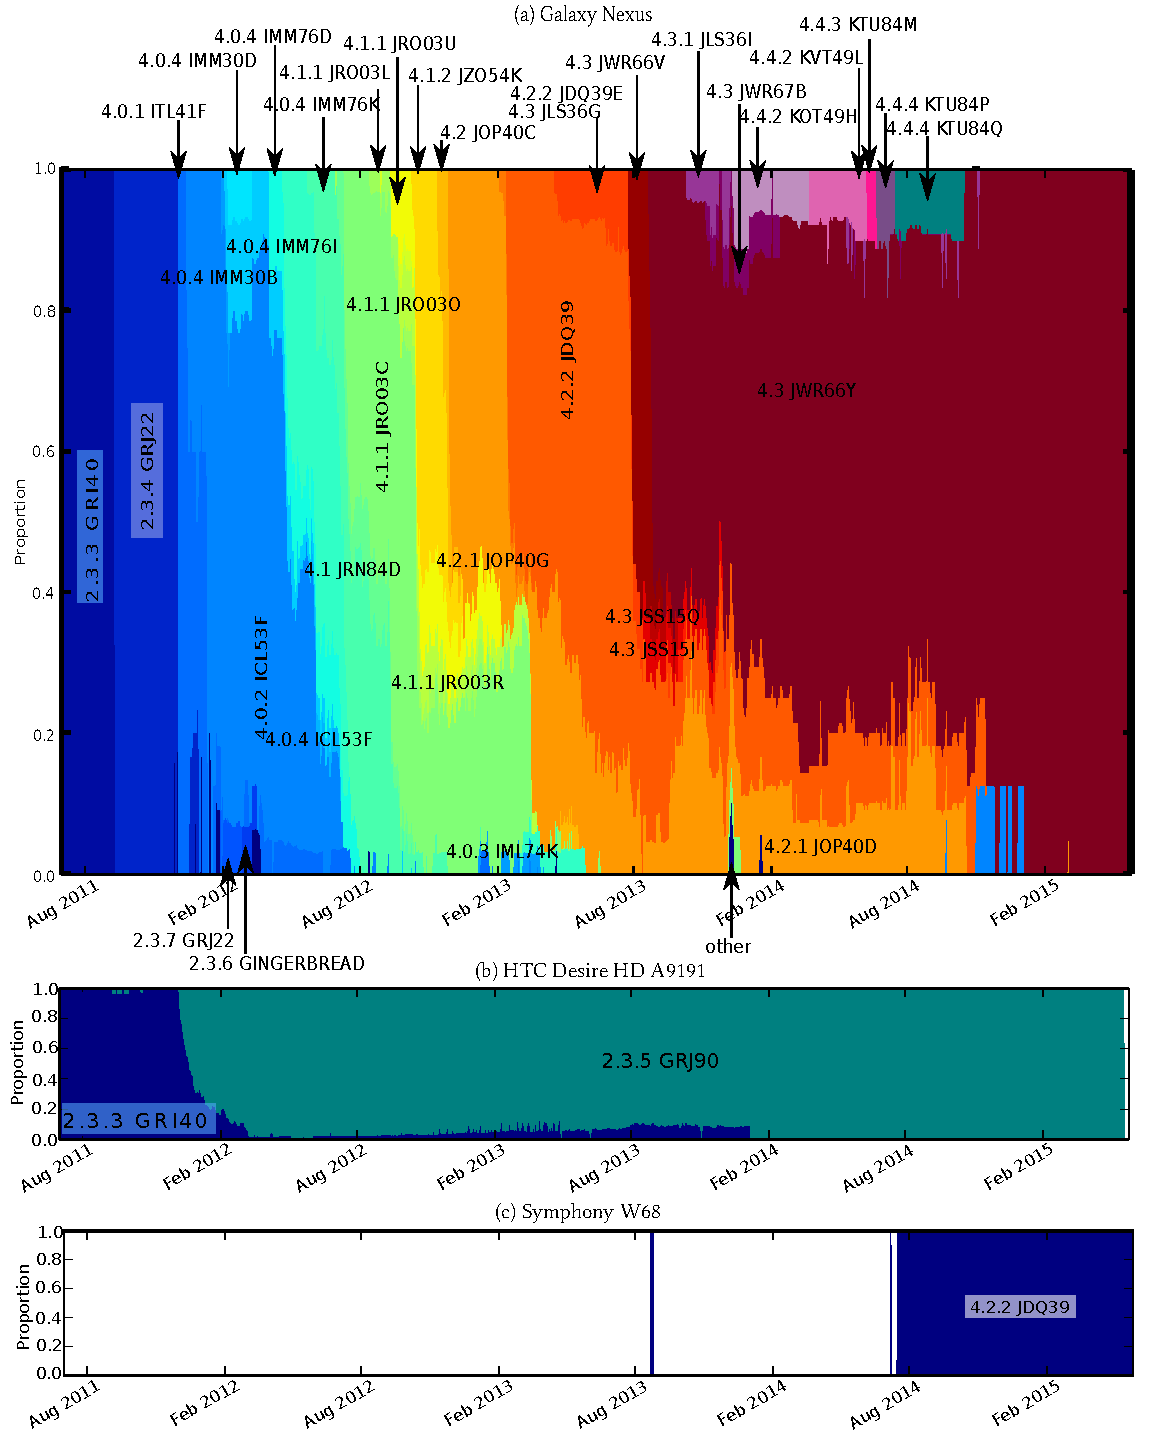
\includegraphics[width=0.9\textwidth]{figures/full_version_comp.pdf}
 \caption{Full version distributions for the highest and lowest scoring models}
 \label{fig:full_version_comp}
\end{figure*}

\daTabSecScoresoperator
We also analysed different network operators, for the \daNumSigOperators\ network operators with a significant presence in our data.
Table~\ref{tab:sec_operator} shows the results \emph{\daSecScoreBestoperator} (\daSecScoreBestoperatorScore\ out of 10) scoring highest and \emph{\daSecScoreWorstoperator} (\daSecScoreWorstoperatorScore\ out of 10) scoring lowest.
However the score of a network operator is affected by the device manufacturers of the devices which are in use on its network.
This is in turn affected by both what devices a network operator offers to users and upon which devices users choose.
Hence having a worse score does not necessarily mean that a network operator is worse, it could be that its users all pick phones from a worse device manufacturer, for example because they were cheaper.
A network operator could use data from this paper to exclude insecure devices from those offered to consumers.
An added value analysis of network operators which takes into account the device mix used by users of that network operator would make it possible to determine whether a network operator is making the situation better or worse by the way it ships updates to users.
However our sample size is too small to do that as while we have significant numbers of devices for each of the device models (Table~\ref{tab:sec_model}) and for each of the network operators (Table~\ref{tab:sec_operator}) we would need a significant number of each model in each network operator.
%We do not attempt to disambiguate users behaviour in whether they install updates from network operators using rolling upgrades.


\subsection{Scores over time}
\begin{figure}
\centering
\begin{subfigure}{\columnwidth}
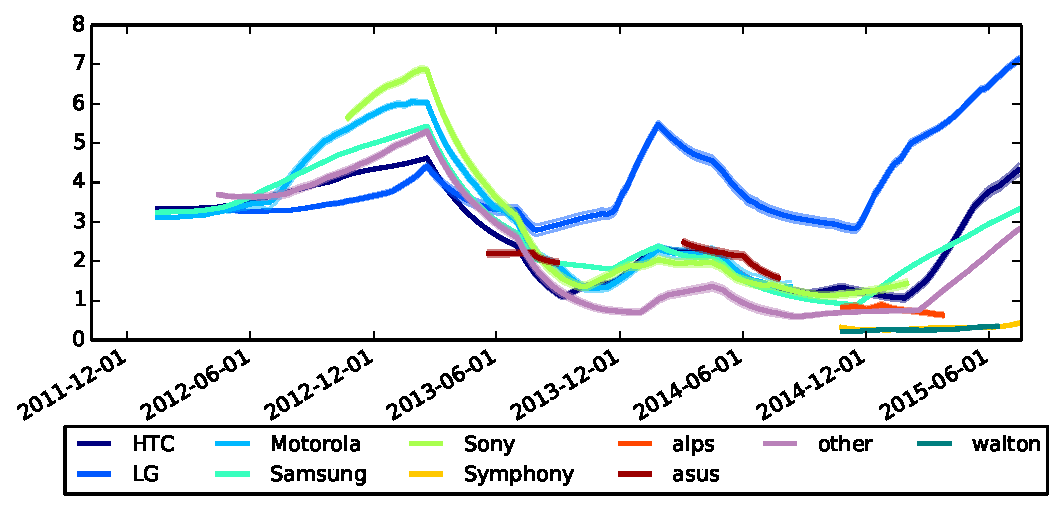
\includegraphics[width=\columnwidth]{figures/security_score_manufacturer}
\caption{Device manufacturers}
\label{fig:security_score_manufacturer}
\end{subfigure}
%
\begin{subfigure}{\columnwidth}
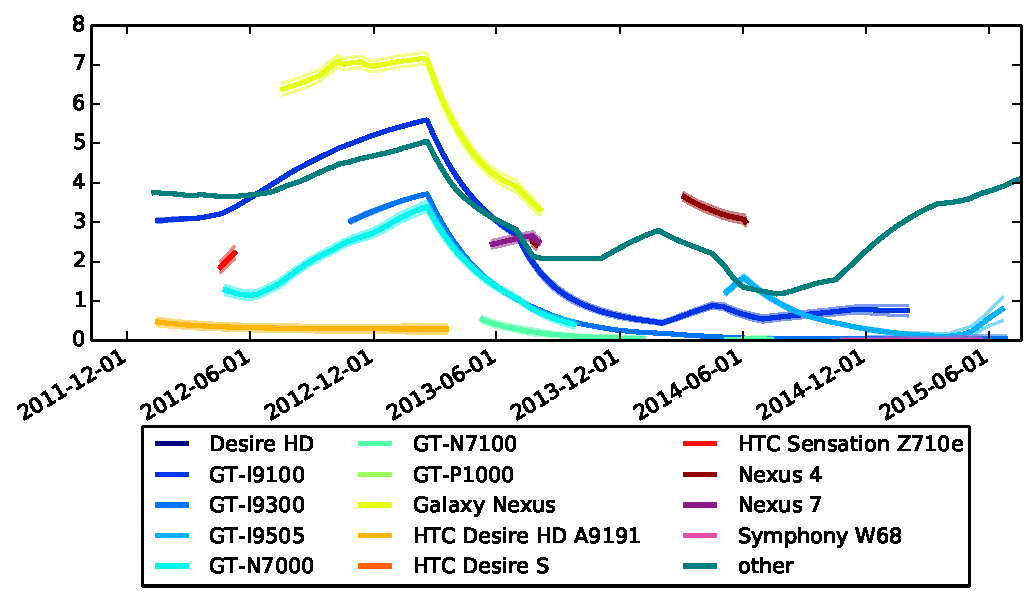
\includegraphics[width=\columnwidth]{figures/security_score_model}
\caption{Device models}
\label{fig:security_score_model}
\end{subfigure}
%
\begin{subfigure}{\columnwidth}
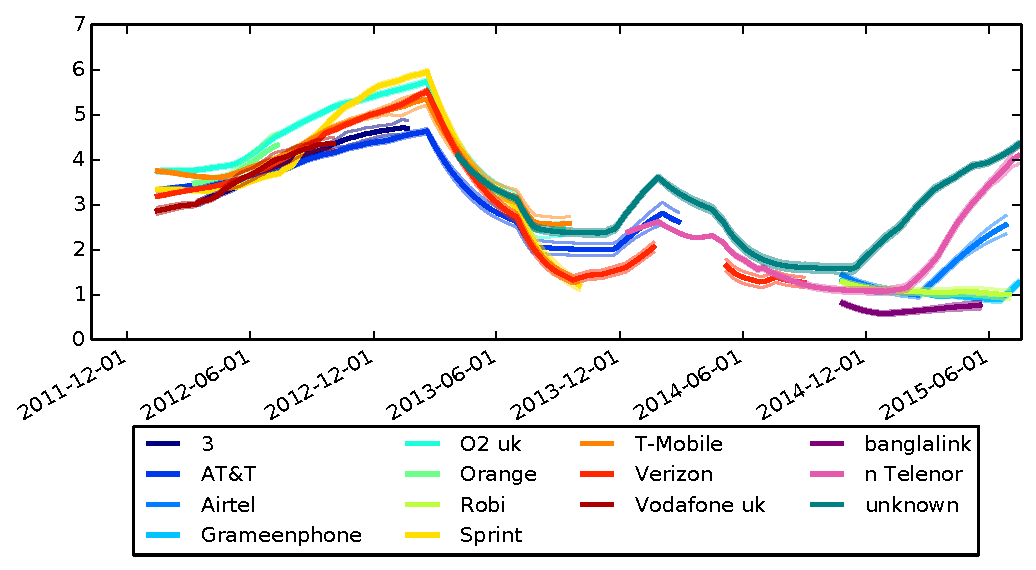
\includegraphics[width=\columnwidth]{figures/security_score_operator}
\caption{Network operators}
\label{fig:security_score_operator}
\end{subfigure}
%
\begin{subfigure}{\columnwidth}
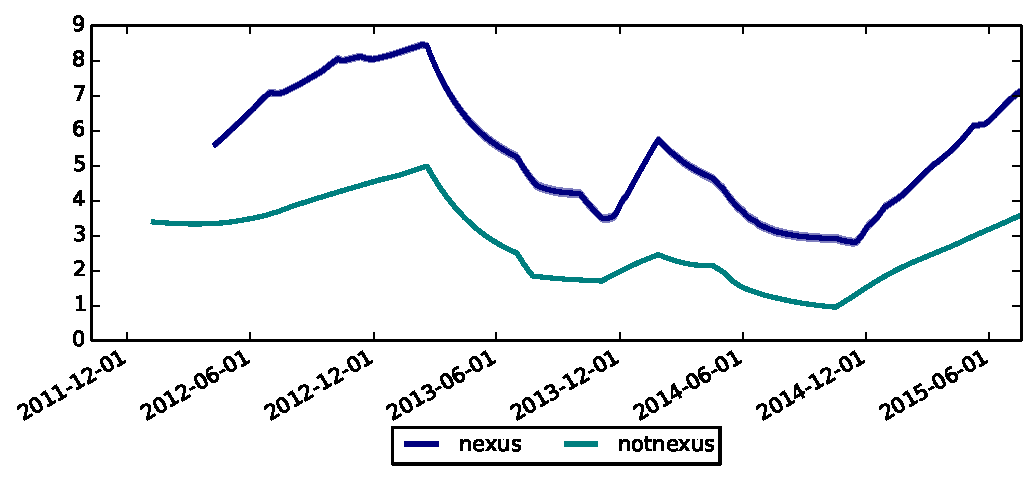
\includegraphics[width=\columnwidth]{figures/security_score_summary}
\caption{Nexus and non-Nexus devices}
\label{fig:security_score_summary}
\end{subfigure}
\caption{Security scores for device manufacturers, device models, network operators and Nexus devices. 95\% confidence intervals indicated.\todolater{bridge gaps?}}
\label{fig:security_scores}
\end{figure}
\todo{This is method rather than result}
The scoring metric as originally computed is averaged over the whole history of the device manufacturer, device model or network operator, it gives equal weight to periods years ago as to in the last few months.
If instead we take an exponential moving average of the daily score for days with more than \daSigNumDevicesDay\ devices when there have been at least consecutive \daSigNumDays\ days of data with that many devices then we can plot how this score has changed over time.
Equation~\ref{eq:rolling_update} shows how the value for a particular day ($v_i$) is computed from the previous day's value and the input for the current day ($n$) with an $\alpha$ of $1/\daSigNumDays$.
\begin{equation}
v_i = v_{i-1} (1 - \alpha) + n \alpha
\label{eq:rolling_update}
\end{equation}
Figure~\ref{fig:security_scores} shows this for manufacturers, device models, network operators and for Nexus and non-Nexus devices.
These show how the scores for different entities are different and change over time, while there is correlated behaviour for different entities (due to things like new vulnerabilities affecting all Android being discovered) these lines still have crossings due to the different behaviour of the different entities.
It also shows that we do not have sufficient data for all the entities all of the time, resulting in gaps in the data.
The clearest results are for Figure~\ref{fig:security_score_summary} with a large gap between the scores for Nexus and non-Nexus devices across the whole data set.


\subsection{Sensitivity of scoring metric}
\daTabDLDistances
\daTabChangeInScores
To evaluate whether the ranking of different manufacturers is sensitive to the form of the scoring metric we computed the normalised Damerau-Levenshtein distance~\cite{Bard2007} between the lists ordered using different forms of the scoring metric, this is shown in Table~\ref{tab:dl_distances}.
The `equal' metric weights $f$, $u$ and $m$ equally rather than favouring $f$ and makes little difference.
Changing the scoring metric also impacts the scores given for each entity Table~\ref{tab:change_in_scores} shows the mean impact on the scores.
This shows that $m$ tends to drag down scores.
\todo{Give some of the actual orderings as well for the most important ones}
\todo{Sensitivity of time based vs. global scores}

\subsection{Gaming the score}
If the comparative data given here is used to influence purchasing decisions then entities in the Android ecosystem might try to game the score rather than genuinely improve security.
$f$ is hard to game without doing a good job at security but it doesn't get any worse if there is already one known vulnerability and another is found.
A high value of $u$ could be achieved by only ever shipping one version but that would give low values for $f$ and $m$ (and not be attractive to new customers).
A high value of $m$ could be achieved by focusing on only one device at a time and ensuring that it gets updates but ignoring all others, but that would lower $f$ and $u$.%
One way to influence our scores would be to add additional devices to Device Analyzer which have good security, these would have to be real end user devices as we could detect fake ones, this would increase the size of our data set and would require providing genuinely good security to some users.
Therefore our score is secure against passive gaming attacks which changed the measured distribution but would require active defence against active gaming attacks which target the measurement devices.


\section{Threats to validity}
\label{sec:validity}
\subsection{The \da\ data gives a conservative estimate of the Android version distribution}
\label{sec:representative}
\begin{figure}
 \centering
 \begin{subfigure}[b]{\columnwidth}
 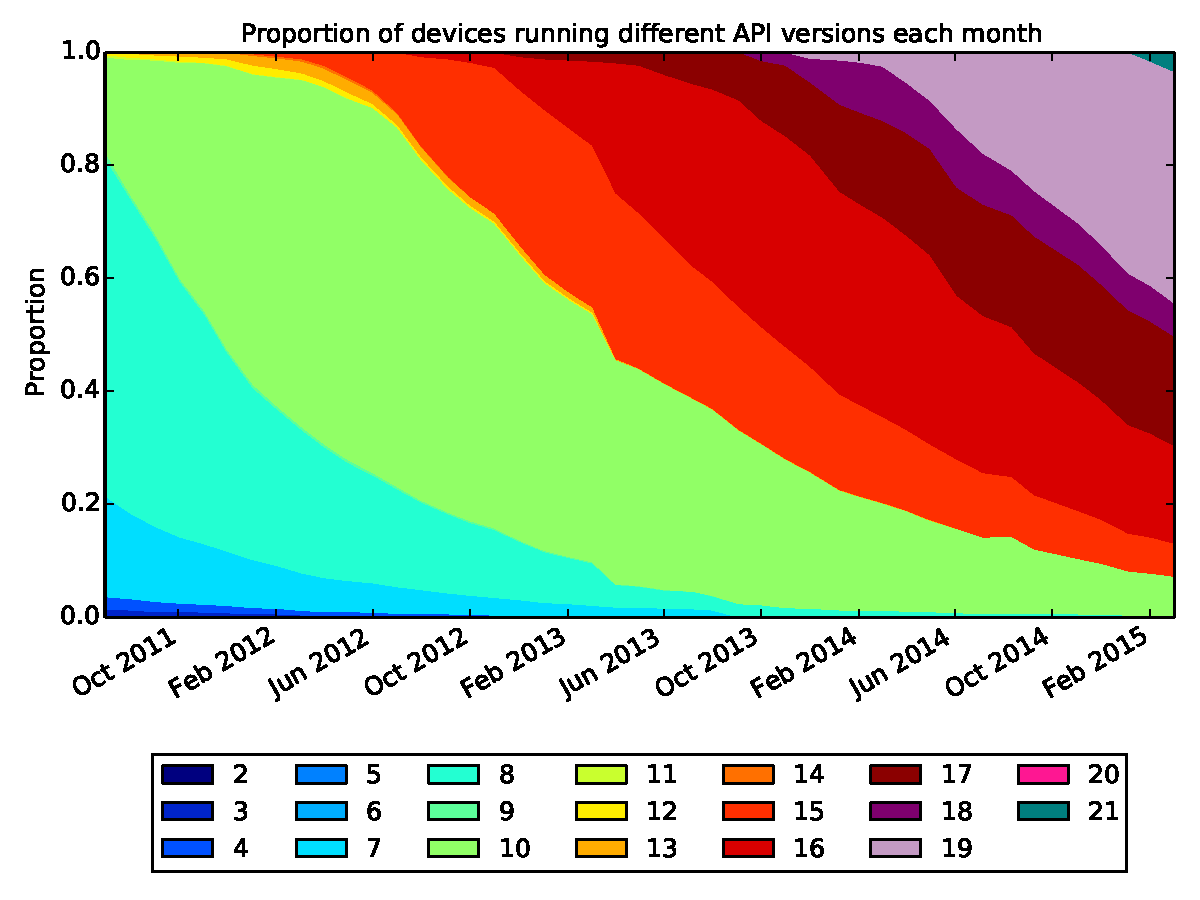
\includegraphics[width=\columnwidth]{figures/googleplayapi}
 \caption{Google Play data on proportion of devices running different Android API versions}
 \label{fig:play_api}
\end{subfigure}
\begin{subfigure}[b]{\columnwidth}
 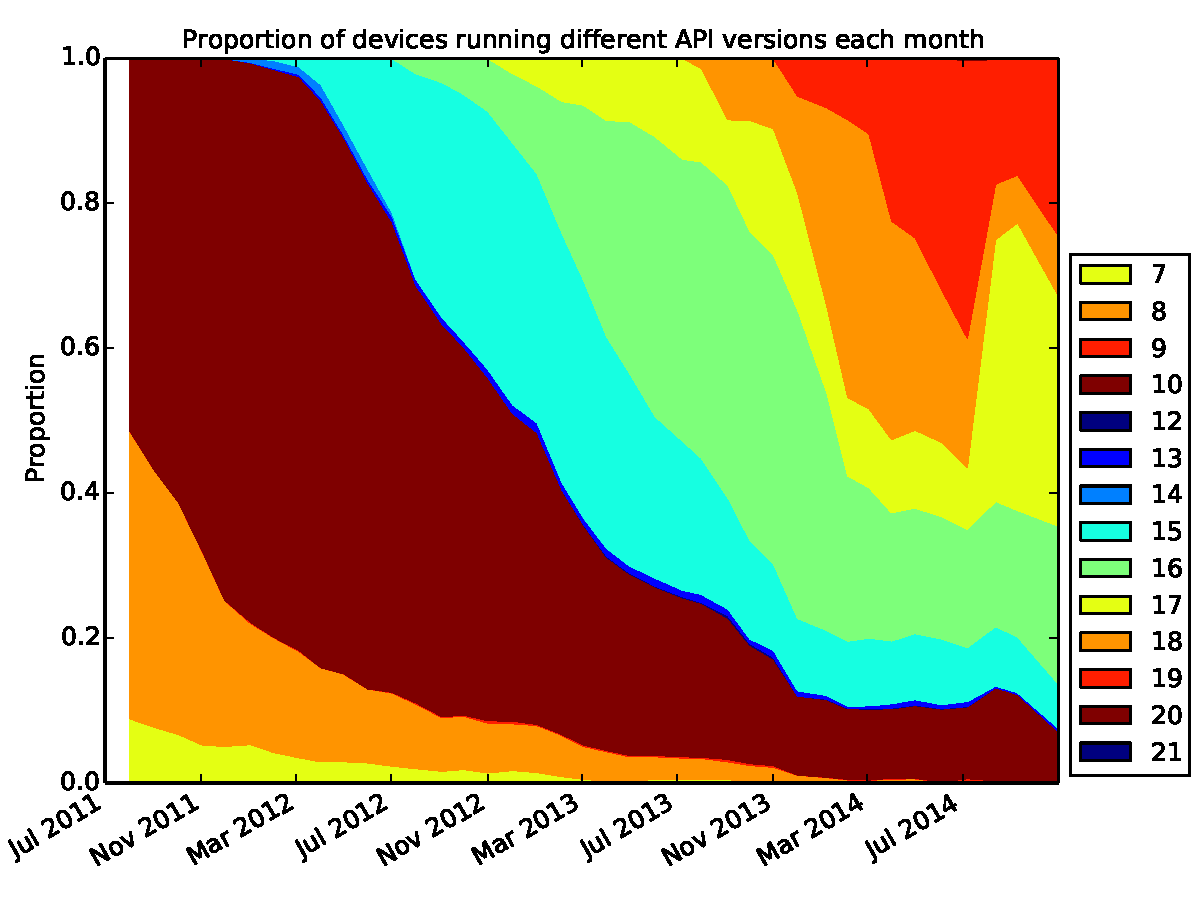
\includegraphics[width=\columnwidth]{figures/norm_api_gpcomp}
 \caption{\da\ data on proportion of devices running different Android API versions}
 \label{fig:da_api}
\end{subfigure}
\caption{Monthly Android API version data}
\end{figure}
\begin{figure}
 \centering
 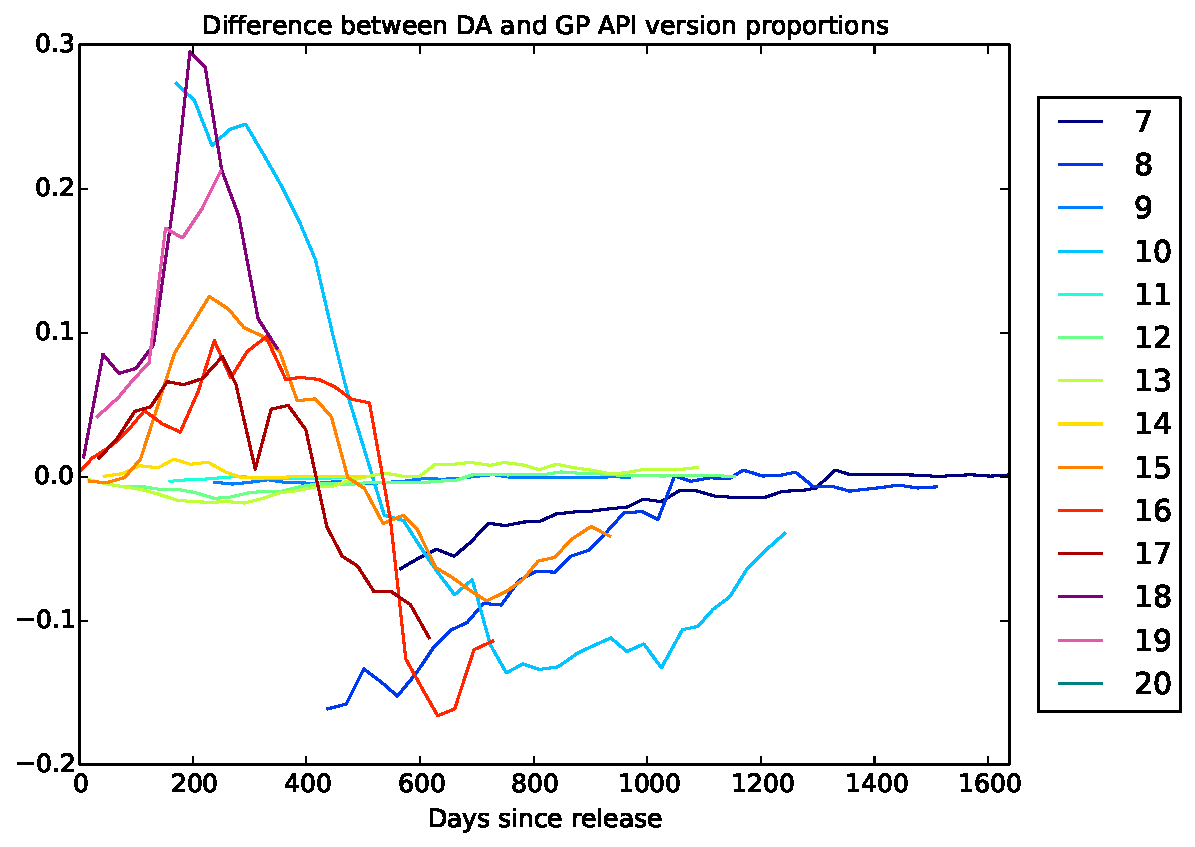
\includegraphics[width=\columnwidth]{figures/api_gpcomp_rdiff}
 \caption{Difference between \da\ and Google Play data on the proportion of devices running different Android API versions}
 \label{fig:da_gp_comp_diff}
\end{figure}
The data from \da\ we used to investigate the proportion of devices exposed to different vulnerabilities is the OS version.
Unfortunately there is no authoritative source of OS version information and so we cannot check directly whether our data is representative.
However Google has published API version information every month since December 2009 and we have collated this information.\footnote{\url{http://androidvulnerabilities.org/play/historicplaydashboard}}
While API versions are too coarse grained to use for security update detection they are closely related to OS versions and so if the \da\ data on API versions is similar to the Google Data on API versions then the \da\ data on OS versions should be representative.
Figure~\ref{fig:play_api} shows the data from Google and Figure~\ref{fig:da_api} shows the data from \da\ and they appear similar.
Figure~\ref{fig:da_gp_comp_diff} shows the difference between Figures~\ref{fig:play_api} and \ref{fig:da_api}, normalising for days since the API version was released.
It shows that the \da\ data systematically overestimates the prevalence of new API versions and underestimates the prevalence of old API versions.
This means that the OS version information from \da\ is likely to be overestimating the prevalence of new OS versions and hence our results are a conservative estimate of the security of Android.
\todolater{we want a statistical metric to claim this strongly with.}
This allows us to have confidence in the OS version information.


\subsection{Changes in the \da\ sample}
\label{sec:da_changes}
The \da\ data is mostly generated by devices which have the \da\ app installed because their owner happened to come across the app on Google Play as there has been no advertising and few other attempts to increase usage.
However two collaborations with network operators to install \da\ on customer devices resulted in large numbers of new \da\ users coming from particular areas and network operators.
One study was conducted in Norway with 654 installs of \da\ and one was conducted in Bangladesh where 2463 users installed \da.
This is responsible for the sudden change in distribution of OS versions in \da\ shown towards the end of Figures \ref{fig:norm_os}, \ref{fig:nvulnerabilities_heat} and \ref{fig:proportioninsecure} as for that period Bangladeshi users contributed over half of the \da\ data.
%We could normalise out the influence of the Bangladeshi users, however they are Android users too and they also need security updates.
Since most \da\ users are self selecting and install \da\ because they want to find out more about what their phone is doing or to aid research they may be biased and perhaps more likely to install updates.


\section{Discussion} \label{sec:discussion}
There are continuing efforts to reduce the impact of critical vulnerabilities, both in Android and more widely.
SEAndroid~\cite{Smalley2013} which is included in Android from version 4.1~\cite{jelly-bean-release} claimed to prevent some root vulnerabilities and to reduce the impact of others.
Capability based enforcement systems such as Capsicum~\cite{Watson2010} substantially reduce the capabilities that an exploit has to try and gain increased privilege with.
When Capsicum is included in Linux\footnote{\url{https://github.com/google/capsicum-linux}} and hence in Android, it could be used to place fine grained restrictions on system daemons, preventing vulnerabilities becoming critical vulnerabilities.

We have not included all the vulnerabilities from \avo\, in particular we have not included any device manufacturer specific vulnerabilities, even when these are widespread (such as vulnerabilities affecting Qualcomm\footnote{Qualcomm is particularly good at publicly disclosing the vulnerabilities affecting their code and the patches which fix them. \url{https://www.codeaurora.org/projects/security-advisories/}} chipsets) because it is difficult to work out which devices are affected.
There also tends to be less public information available about device manufacturer specific vulnerabilities which makes them harder to tie down.
For other vulnerabilities which might affect all Android devices it is hard to work out which devices they affect.
For example \emph{pty race}\footnote{\url{http://androidvulnerabilities.org/vulnerabilities/pty_race}} is a Linux kernel vulnerability, we found 48 commits which fixed it in different branches, it was also accidentally fixed and later reintroduced and so determining which devices were vulnerable relies on knowing where on which branch the kernel was taken from.
For some vulnerabilities the corresponding patch is not in AOSP despite some device manufacturers having shipped builds containing the fix, which makes working out what is going on more difficult.
For \emph{RageAgainstTheCage adb}\footnote{\url{http://androidvulnerabilities.org/vulnerabilities/RageAgainstTheCage_adb}} and \emph{keystore buffer}\footnote{\url{http://androidvulnerabilities.org/vulnerabilities/keystore_buffer}} vulnerabilities which we do have sufficient data it is not clear whether they are truly critical vulnerabilities as the former may require physical ADB access and the latter may be protected by a sandbox.
However those two vulnerabilities make little difference to our results as they affect few devices.

\subsection{Open questions}
There are several open questions which we have not yet been able to answer and remain future work.
\begin{itemize}
 \item Why was there a gap in vulnerability discovery in Android in 2012?
 \item Why do so many devices have ADB enabled? \daAdbEnabledPerc\ seems rather high for a developer feature. This could be a selection bias or device manufacturers could be enabling it by default.
 \item How much of updating is new handsets and how much is updates being deployed? Over time newer versions of Android come to dominate, but quantifying what proportion of that is due to new phones being purchased and what proportion is due to updates to existing devices is a question we cannot answer.
 The only available large data set we know of with longitudinal traces of Android devices OS version numbers is \da\ but that only records \daNumUpdatesUpgrades\ upgrades which broken down over \daOSMonthsOfData\ months and \daNumSigOSVersions\ OS versions is only \daUpdatesPerMonthPerVersion\ updates per version per month which is not enough to build a statistically significant prediction of the expected transition to newer versions of Android.
 \item Why do users downgrade their phones?
\end{itemize}


\section{Related work}
\label{sec:related}
Using the methods and data described in this paper we have determined that, on average, \daMeanInsecurityPerc\ of devices were exposed to known critical vulnerabilities between 2011 and 2014.
Felt et al.\ studied 6 Android handsets in 2011 and found they were exposed to root vulnerabilities at least 74\% of the time~\cite{Felt2011} .
Our approach differs from their study because they used data from 6 handsets and assumed the best possible update distribution, while our work is based on a large sample of devices tracking the actual update distribution.
Nevertheless, our own analysis as well as comparison with their work suggests protection against critical vulnerabilities has not improved significantly over the last 3 years. 
Felt et al.\ also found that 4 of the 46 malware samples (8\%) they analysed contained root exploits, much lower than rates found in later (larger) studies which found rates of 36.7\%~\cite{Zhou2012b} and 40\%~\cite{Zhou2012a} in 2012.

Currently, finding and exploiting vulnerabilities is typically a time-consuming and manual process.
Therefore an attacker has to invest significant human resource to first find a bug and then write code to exploit the vulnerability.
To reduce the effort involved in finding a bug, attackers can look at security-related commits made to open source repositories.
Previous work has shown attackers have taken this approach for the Firefox web browser~\cite{Barth2011}.
Google does not release updates to the Android source code until after the release of the relevant security update.
This reduces the time available for an attacker to exploit a vulnerability by looking at security updates disclosed in the source code repository from the period (\textbf{first fix}, \textbf{fix deployed}) to (\textbf{fixing release}, \textbf{fix deployed}).
Unfortunately the time period between the \textbf{fixing release} and \textbf{fix deployed} can be of the order of months. 
For example, the zergRush vulnerability was fixed in a release before it was publicly discovered but it still took 27 months for 90\% of the devices in our study to be definitely fixed\footnote{Definitely fixed is 1 $-$ (definitely insecure + maybe insecure), maybe fixed is 1 $-$ definitely insecure} (25 months for 90\% of devices maybe fixed).

Recent work by Brumley et al. has shown it is possible to automatically generate exploits from binary fixes, for example by using security updates issued by manufacturers~\cite{Brumley2008}. 
Similarly, the Woodpecker tool automatically finds permission leaks in stock Android phone images~\cite{Grace2012}.
Once such automated techniques mature, it will become even more important to provide security updates promptly to every Android device in the ecosystem because an attacker can turn the contents of a \textbf{fixing release} into an exploit in a matter of minutes or hours.

Security in depth is also a useful strategy.
In this regard, iOS provides additional safeguards beyond those used in Android, including a pre-distribution code review, mandatory code-signing by the manufacturer, and (with the important exception of ROP-based attacks~\cite{Wang2013a}) the technical prohibition of dynamic code loading by an app.
These features, as well as Address Space Layout Randomisation (ASLR) and mandatory access controls, has resulted in a lower level of malware affecting iOS when compared to Android~\cite{Felt2011}.

Rather than fixing critical vulnerabilities, security can be obtained by detect them and preventing the installation or execution of malicious apps.
Detection strategies include RiskRanker, which classified 3\,281 out of 118\,318 apps (2.8\%) as risky of which 718 (22\%) were malware and 322 (10\%) were previously unknown malware, an overall infection rate of 0.6\% across multiple markets~\cite{Grace2012a}.
DroidRanger also analysed apps finding 148 out of 182\,823 apps (0.08\%) to be malicious across multiple markets of which 29 were previously unknown~\cite{Zhou2012a}.
%DroidRanger: It used permission-based behavioural fingerprinting which looked at the permissions of known malware and heuristic-based filtering -- dynamic loading of both Dalvik and native code.
A common technique used by attackers takes existing popular apps and repackages them to include malicious code. 
AnDarwin uses this insight to detect similar apps, and found 169 out of 265\,359 of all apps studied (0.06\%) were malicious clones of genuine apps~\cite{Crussell2013}.
%AnDarwin: It used clustering based on semantic vectors derived from the program dependence graphs to detect similar apps.

Unfortunately, whilst these tools were successful in finding critical vulnerabilities, such techniques are not perfect.
The Malware Genome project collected 1\,260 malware samples from 2010--2011~\cite{Zhou2012b}.
They found that the best case for anti-malware detection on their data was 79.6\%.
Similarly, DroidChameleon found that antivirus products could not detect malware if the execution binary was automatically permuted~\cite{Rastogi2013}.
Therefore detecting risky apps which might contain critical vulnerabilities is a useful tool, but it does not replace the need to provide security updates.

%All these app analysis projects have been hampered by the difficulty of obtaining full datasets of Android apps as Google does not make these available (and researchers who automatically download them violate Google's Terms of Service).
%PlayDrone was a particularly effective project which circumvented Google's protective measures and downloaded over 1\,100\,000 apps from Google Play, allowing an in depth analysis~\cite{Viennot2014}.

The update process for apps, security fixes and OS upgrades also needs to be secure.
Unfortunately, package management systems designed to provide secure updates have been found to contain vulnerabilities~\cite{Cappos2008} and many software update systems fail to authenticate the connection between the device and the update server or do not authenticate the downloaded binaries~\cite{Bellissimo2006}.
Android does authenticate update binaries and Google Play downloads them over a secure connection~\cite{Viennot2014}.
In this paper we have analysed four critical vulnerabilities in the Android app update mechanism: APK unsigned shorts, APK unchecked name, APK duplicate file and Fake ID.
Other work has demonstrate complex and subtle errors exist in the Android app update process.
For example, the process can be exploited to allow apps to gain privilege through `Pileup' vulnerabilities by registering for new permissions before the update which creates that permission is installed~\cite{Xing2014}.

The percentage of Android devices running the most recent version (\daUpdatednessPerc) compares unfavourably with the rate ($>90$\%) for Windows XP SP2 computers contacting the Microsoft update servers~\cite{Gkantsidis2006}.
A simple numerical comparison is unfair because only one major OS version was considered in the Microsoft analysis, and data was only collected from computers which contacted the update server, although this was the default.
More recent data demonstrates the difficulty of upgrading computers between major OS versions, with 27\% of Windows computers running Windows XP in July 2014,\footnote{\url{https://archive.today/PLGxn}} four months after Windows XP stopped receiving security updates.

User-Agent strings have been used to investigate the timeliness of web browser updates~\cite{Frei2008}, with at most 80\% of Firefox users running the most recent version.
The same analysis was used to show that Chrome's use of silent updates seems to increase uptake of upgrades~\cite{Duebendorfer2010} with 97\% of users running the latest version within 3 weeks of release.
By way of comparison, Android's update process is manual.
The user is notified an update exists, but further action is required, including downloading the update and rebooting the phone to enable installation.
The phone must have sufficient charge to perform the update and the device itself is rendered inoperable during the update process, two factors which might prevent or delay the update process from taking place.
In our data we are unable to determine why a device is not updated. 
It is possible that many updates arrive at handsets, but are simply not installed.
Anecdotal evidence at least suggests that it is the lack of updates rather the lack of installation which is the major problem at present. Further work is required to tease these numbers apart.
%Partly this is the result of the fact that an operating system update is being installed and so a reboot is required, but Chrome installs the new version side by side with the old one and switches the next time it is restarted.
%The same technique would be more difficult on phones with limited storage space (as many cheap Android phones have barely enough space to install just the update) but is a plausible improvement for more high-end devices.
%Google is deploying the same silent update technique through Google Play Services\footnote{\href{http://lifehacker.com/why-google-play-services-are-now-more-important-than-an-975970197}{http://lifehacker.com/why-google-play-services-are-now-more-important-than-an-975970197}} which automatically installs updates for core Google components of Android, this also bypasses the device manufacturer and network operator.



\section{Conclusion}
\label{sec:conclusion}
We have investigated the security of the Android operating system with respect to security updates and examined how the Android ecosystem results in different device models receiving different levels of security due to whether or not they get security updates.
We have compared different device models, device manufacturers and network operators and found that there are differences between them which the discerning purchaser might use to influence their decision about which device model to buy from which device manufacturer and network operator.
We hope that this analysis will encourage device manufacturers and network operators to improve the support they provide for devices after sale.
Android attempts to provide good security to end users through sandboxing apps.
However the latency in the security update process means that on average \daMeanInsecurityPerc\ of Android devices are exposed to known critical vulnerabilities which break out of the sandbox and only \daUpdatednessPerc\ of devices run the latest version of Android.

\identifying{
\section*{Acknowledgements}
Thanks to Richard Clayton, the mobile security reading group and Anil Madhavapeddy for reading various drafts of this paper.
Thanks to David Robertson for helpful advice on statistical analysis.
Thanks to Laurent Simon, Thomas Coudray, Adrian Taylor, Justin Case, Giant Pune and Khilan Gudka for reporting vulnerabilities in Android.
}

\printbibliography


\listoftodos


\end{document}
